\documentclass[11pt,a4paper]{article}

%--------------------------------------------------------------------------
% MinionPro fonts
%--------------------------------------------------------------------------
\IfFileExists{MinionPro.sty}{%
  \usepackage[mnsy]{MnSymbol}
  \usepackage{MinionPro}
  \usepackage{MyriadPro}
  \DeclareSymbolFont{eulerletters}{U}{zeur}{m}{n}
  \DeclareMathSymbol{0}{\mathord}{eulerletters}{`0}
}{%
  \usepackage[T1]{fontenc}
  \usepackage{newtxtext}
  %\usepackage{eulervm}
  \usepackage{amssymb}%needed for \mathbb
}

\input{./ParresiaResearchReportStyle.tex}     
\usepackage[backend=biber,style=authoryear,natbib=true,hyperref=true,backref=true]{biblatex}
\PassOptionsToPackage{hyphens}{url}\usepackage[pdftex,a4paper=true,colorlinks=true,linkcolor=blue,urlcolor=blue,citecolor=blue]{hyperref}
\usepackage{longtable}
\usepackage{listings}
\usepackage{animate}
\usepackage{parskip}
\usepackage[toc,page]{appendix}
\definecolor{red}{rgb}{1,0,0}
\definecolor{green}{rgb}{0,1,0}
\definecolor{blue}{rgb}{0,0,1}
\definecolor{Red}{rgb}{0.8666,0.03137,0.02352}
\definecolor{Blue}{rgb}{0.00784,0.67059,0.91764}
\definecolor{Darkgreen}{rgb}{0,0.68235,0}
\definecolor{Green}{rgb}{0,0.8,0}
\definecolor{Bl}{rgb}{0,0.2,0.91764}
\definecolor{Royalblue}{rgb}{0,0.2,0.91764}
\definecolor{Brickred}{rgb}{0.644541,0.164065,0.164065}
\definecolor{Brown}{rgb}{0.6,0.4,0.4}
\definecolor{Orange}{rgb}{1,0.647059,0}
\definecolor{Indigo}{rgb}{0.746105,0,0.996109}
\definecolor{Violet}{rgb}{0.308598,0.183597,0.308598}
\definecolor{Lightgrey}{rgb}{0.762951,0.762951,0.762951}
\definecolor{Darkgrey}{rgb}{0.503548,0.503548,0.503548}
\definecolor{Pink}{rgb}{1,0.6,0.6}
\definecolor{MyLightMagenta}{cmyk}{0.1,0.8,0,0.1}
\definecolor{MyDarkBlue}{rgb}{0,0.08,0.45}
\definecolor{OliveDrab}{rgb}{0.41961,0.55686,0.13725}
\definecolor{OliveD}{HTML}{6B8E23}
\definecolor{ocre}{RGB}{243,102,25}

\newcommand{\Ochre}{\color{ocre}}
\newcommand{\Red}{\color{Brickred}}
\newcommand{\Blue}{\color{Royalblue}}
\newcommand{\Green}{\color{Darkgreen}}
\newcommand{\Violet}{\color{Violet}}
\newcommand{\Indigo}{\color{Indigo}}
\newcommand{\Orange}{\color{Orange}}
\newcommand{\Brown}{\color{Brown}}
\newcommand{\Olive}{\color{OliveD}}

%------------------------------------------------------------------
% Wide bar
%------------------------------------------------------------------
\newcommand{\overbar}[1]{\mkern 1.5mu\overline{\mkern-1.5mu#1\mkern-1.5mu}\mkern 1.5mu}
\renewcommand{\bar}[1]{\overbar{#1}}
\newcommand{\Ibar}{\ensuremath{\bar{I}}}
\newcommand{\Ionebar}{\ensuremath{\bar{I_1}}}
\newcommand{\kappabar}{\ensuremath{\bar{\kappa}}}
\newcommand{\zetabar}{\ensuremath{\bar{\zeta}}}
\newcommand{\Xbar}{\ensuremath{\bar{X}}}

\newcommand{\Jump}[1]{\ensuremath{\llbracket#1\rrbracket}}
\newcommand{\Blimitx}[1]{\ensuremath{\left[#1\right]_{x_a}^{x_b}}}
\newcommand{\Deriv}[2]{\ensuremath{\cfrac{d#1}{d#2}}}
\newcommand{\MDeriv}[2]{\ensuremath{\cfrac{D#1}{D#2}}}
\newcommand{\MDerivalpha}[2]{\ensuremath{\cfrac{D^\alpha#1}{D#2}}}
\newcommand{\MDerivbeta}[2]{\ensuremath{\cfrac{D^\beta#1}{D#2}}}
\newcommand{\MDerivsolid}[2]{\ensuremath{\cfrac{D^s#1}{D#2}}}
\newcommand{\MDerivwater}[2]{\ensuremath{\cfrac{D^w#1}{D#2}}}
\newcommand{\MDerivair}[2]{\ensuremath{\cfrac{D^a#1}{D#2}}}
\newcommand{\DDeriv}[2]{\ensuremath{\cfrac{d^2#1}{d#2^2}}}
\newcommand{\DDDeriv}[2]{\ensuremath{\cfrac{d^3#1}{d#2^3}}}
\newcommand{\Intx}{\ensuremath{\int_{x_a}^{x_b}}}
\newcommand{\IntX}{\ensuremath{\int_{X_a}^{X_b}}}
\newcommand{\Intiso}{\ensuremath{\int_{-1}^{1}}}
\newcommand{\IntOmegaA}{\ensuremath{\int_{\Omega_0}}}
\newcommand{\IntOmega}{\ensuremath{\int_{\Omega}}}
\newcommand{\Abs}[1]{\ensuremath{\left|#1\right|}}
\newcommand{\Norm}[2]{\ensuremath{\stretchleftright{\lVert}{#1}{\rVert}_{#2}}}
\newcommand{\NormL}[2]{\ensuremath{\Big\lVert#1\Big\rVert_{#2}}}
\newcommand{\Var}[1]{\ensuremath{\delta #1}}
\newcommand{\DelT}{\ensuremath{\Delta t}}
\newcommand{\CalA}{\ensuremath{\mathcal{A}}}
\newcommand{\CalB}{\ensuremath{\mathcal{B}}}
\newcommand{\CalC}{\ensuremath{\mathcal{C}}}
\newcommand{\CalD}{\ensuremath{\mathcal{D}}}
\newcommand{\CalE}{\ensuremath{\mathcal{E}}}
\newcommand{\CalF}{\ensuremath{\mathcal{F}}}
\newcommand{\CalG}{\ensuremath{\mathcal{G}}}
\newcommand{\CalH}{\ensuremath{\mathcal{H}}}
\newcommand{\CalK}{\ensuremath{\mathcal{K}}}
\newcommand{\CalL}{\ensuremath{\mathcal{L}}}
\newcommand{\CalM}{\ensuremath{\mathcal{M}}}
\newcommand{\CalN}{\ensuremath{\mathcal{N}}}
\newcommand{\CalP}{\ensuremath{\mathcal{P}}}
\newcommand{\CalS}{\ensuremath{\mathcal{S}}}
\newcommand{\CalV}{\ensuremath{\mathcal{V}}}
\newcommand{\CalW}{\ensuremath{\mathcal{W}}}
\newcommand{\CalX}{\ensuremath{\mathcal{X}}}
\newcommand{\Comp}[2]{\ensuremath{#1 \circ #2}}
\newcommand{\Map}[3]{\ensuremath{#1 : #2 \rightarrow #3}}
\newcommand{\MapTo}[3]{\ensuremath{#1 : #2 \mapsto #3}}
\newcommand{\Real}[1]{\ensuremath{\mathbb{R}^{#1}}}
\newcommand{\Veps}{\ensuremath{\varepsilon}}
\newcommand{\Ve}{\ensuremath{\varepsilon}}
\newcommand{\BHat}[1]{\ensuremath{\hat{\boldsymbol{#1}}}}
\newcommand{\BTx}{\ensuremath{\tilde{\boldsymbol{x}}}}
\newcommand{\Beh}{\ensuremath{\hat{\boldsymbol{e}}}}
\newcommand{\BHex}{\ensuremath{\hat{\boldsymbol{e}}_1}}
\newcommand{\BHey}{\ensuremath{\hat{\boldsymbol{e}}_2}}
\newcommand{\BHez}{\ensuremath{\hat{\boldsymbol{e}}_3}}
\newcommand{\BHn}[1]{\ensuremath{\hat{\boldsymbol{n}}_{#1}}}
\newcommand{\BHe}[1]{\ensuremath{\hat{\boldsymbol{e}}_{#1}}}
\newcommand{\BHg}[1]{\ensuremath{\hat{\boldsymbol{g}}_{#1}}}
\newcommand{\BHG}[1]{\ensuremath{\hat{\boldsymbol{G}}_{#1}}}
\newcommand{\Hn}{\ensuremath{\hat{\boldsymbol{n}}}}
\newcommand{\Mba}{\ensuremath{\mathbf{a}}}
\newcommand{\Mbb}{\ensuremath{\mathbf{b}}}
\newcommand{\Mbd}{\ensuremath{\mathbf{d}}}
\newcommand{\Mbf}{\ensuremath{\mathbf{f}}}
\newcommand{\Mbr}{\ensuremath{\mathbf{r}}}
\newcommand{\Mbu}{\ensuremath{\mathbf{u}}}
\newcommand{\Mbv}{\ensuremath{\mathbf{v}}}
\newcommand{\Mbx}{\ensuremath{\mathbf{x}}}
\newcommand{\MbA}{\ensuremath{\mathbf{A}}}
\newcommand{\MbB}{\ensuremath{\mathbf{B}}}
\newcommand{\MbC}{\ensuremath{\mathbf{C}}}
\newcommand{\MbD}{\ensuremath{\mathbf{D}}}
\newcommand{\MbI}{\ensuremath{\mathbf{I}}}
\newcommand{\MbK}{\ensuremath{\mathbf{K}}}
\newcommand{\MbM}{\ensuremath{\mathbf{M}}}
\newcommand{\MbN}{\ensuremath{\mathbf{N}}}
\newcommand{\MbR}{\ensuremath{\mathbf{R}}}
\newcommand{\MbT}{\ensuremath{\mathbf{T}}}
\newcommand{\MbU}{\ensuremath{\mathbf{U}}}
\newcommand{\MbX}{\ensuremath{\mathbf{X}}}
\newcommand{\Mbone}{\ensuremath{\mathbf{1}}}
\newcommand{\Mbzero}{\ensuremath{\mathbf{0}}}
\newcommand{\MbSig}{\ensuremath{\boldsymbol{\sigma}}}
\newcommand{\Mb}{\ensuremath{\left[\mathsf{b}\right]}}
\newcommand{\Mu}{\ensuremath{\left[\mathsf{u}\right]}}
\newcommand{\Mv}{\ensuremath{\left[\mathsf{v}\right]}}
\newcommand{\Mw}{\ensuremath{\left[\mathsf{w}\right]}}
\newcommand{\Mx}{\ensuremath{\left[\mathsf{x}\right]}}
\newcommand{\MA}{\ensuremath{\left[\mathsf{A}\right]}}
\newcommand{\MB}{\ensuremath{\left[\mathsf{B}\right]}}
\newcommand{\MC}{\ensuremath{\left[\mathsf{C}\right]}}
\newcommand{\MD}{\ensuremath{\left[\mathsf{D}\right]}}
\newcommand{\MI}{\ensuremath{\left[\mathsf{I}\right]}}
\newcommand{\ML}{\ensuremath{\left[\mathsf{L}\right]}}
\newcommand{\MM}{\ensuremath{\left[\mathsf{M}\right]}}
\newcommand{\MN}{\ensuremath{\left[\mathsf{N}\right]}}
\newcommand{\MP}{\ensuremath{\left[\mathsf{P}\right]}}
\newcommand{\MQ}{\ensuremath{\left[\mathsf{Q}\right]}}
\newcommand{\MR}{\ensuremath{\left[\mathsf{R}\right]}}
\newcommand{\MT}{\ensuremath{\left[\mathsf{T}\right]}}
\newcommand{\Mone}{\ensuremath{\left[\mathsf{1}\right]}}
\newcommand{\Mzero}{\ensuremath{\left[\mathsf{0}\right]}}
\newcommand{\SfA}{\ensuremath{\boldsymbol{\mathsf{A}}}}
\newcommand{\SfC}{\ensuremath{\boldsymbol{\mathsf{C}}}}
\newcommand{\SfD}{\ensuremath{\boldsymbol{\mathsf{D}}}}
\newcommand{\SfI}{\ensuremath{\boldsymbol{\mathsf{I}}}}
\newcommand{\SfL}{\ensuremath{\boldsymbol{\mathsf{L}}}}
\newcommand{\SfS}{\ensuremath{\boldsymbol{\mathsf{S}}}}
\newcommand{\SfT}{\ensuremath{\boldsymbol{\mathsf{T}}}}
\newcommand{\Msig}{\ensuremath{\left[\boldsymbol{\sigma}\right]}}
\newcommand{\Meps}{\ensuremath{\left[\boldsymbol{\varepsilon}\right]}}
\newcommand{\Ex}{\ensuremath{\boldsymbol{e}_1}}
\newcommand{\Ey}{\ensuremath{\boldsymbol{e}_2}}
\newcommand{\Ez}{\ensuremath{\boldsymbol{e}_3}}
\newcommand{\Exp}{\ensuremath{\boldsymbol{e}^{'}_1}}
\newcommand{\Eyp}{\ensuremath{\boldsymbol{e}^{'}_2}}
\newcommand{\Ezp}{\ensuremath{\boldsymbol{e}^{'}_3}}
\newcommand{\Epsxx}{\ensuremath{\varepsilon_{11}}}
\newcommand{\Epsyy}{\ensuremath{\varepsilon_{22}}}
\newcommand{\Epszz}{\ensuremath{\varepsilon_{33}}}
\newcommand{\Epsyz}{\ensuremath{\varepsilon_{23}}}
\newcommand{\Epszx}{\ensuremath{\varepsilon_{31}}}
\newcommand{\Epsxy}{\ensuremath{\varepsilon_{12}}}
\newcommand{\Sigxx}{\ensuremath{\sigma_{11}}}
\newcommand{\Sigyy}{\ensuremath{\sigma_{22}}}
\newcommand{\Sigzz}{\ensuremath{\sigma_{33}}}
\newcommand{\Sigyz}{\ensuremath{\sigma_{23}}}
\newcommand{\Sigzx}{\ensuremath{\sigma_{31}}}
\newcommand{\Sigxy}{\ensuremath{\sigma_{12}}}
\newcommand{\Eps}[1]{\ensuremath{\varepsilon_{#1}}}
\newcommand{\Sig}[1]{\ensuremath{\sigma_{#1}}}
\newcommand{\X}{\ensuremath{X_1}}
\newcommand{\Y}{\ensuremath{X_2}}
\newcommand{\Z}{\ensuremath{X_3}}
\newcommand{\Balpha}{\ensuremath{\boldsymbol{\alpha}}}
\newcommand{\Bbeta}{\ensuremath{\boldsymbol{\beta}}}
\newcommand{\Beta}{\ensuremath{\boldsymbol{\eta}}}
\newcommand{\Bchi}{\ensuremath{\boldsymbol{\chi}}}
\newcommand{\Bpsi}{\ensuremath{\boldsymbol{\psi}}}
\newcommand{\Bveps}{\ensuremath{\boldsymbol{\varepsilon}}}
\newcommand{\Bkappa}{\ensuremath{\boldsymbol{\kappa}}}
\newcommand{\Bbeps}{\ensuremath{\bar{\boldsymbol{\varepsilon}}}}
\newcommand{\Bnabla}{\ensuremath{\boldsymbol{\nabla}}}
\newcommand{\Bomega}{\ensuremath{\boldsymbol{\omega}}}
\newcommand{\BOmega}{\ensuremath{\boldsymbol{\Omega}}}
\newcommand{\Bsig}{\ensuremath{\boldsymbol{\sigma}}}
\newcommand{\Bsigbar}{\ensuremath{\overline{\boldsymbol{\sigma}}}}
\newcommand{\BSig}{\ensuremath{\boldsymbol{\Sigma}}}
\newcommand{\Btau}{\ensuremath{\boldsymbol{\tau}}}
\newcommand{\Bvarphi}{\ensuremath{\boldsymbol{\varphi}}}
\newcommand{\phibar}{\ensuremath{\overline{\varphi}}}
\newcommand{\Blambda}{\ensuremath{\boldsymbol{\lambda}}}
\newcommand{\Btheta}{\ensuremath{\boldsymbol{\theta}}}
\newcommand{\Bthetav}{\ensuremath{\mathbf{\theta}}}
\newcommand{\Bgamma}{\ensuremath{\boldsymbol{\gamma}}}
\newcommand{\Bmu}{\ensuremath{\boldsymbol{\mu}}}
\newcommand{\Bxi}{\ensuremath{\boldsymbol{\xi}}}
\newcommand{\Bone}{\ensuremath{\boldsymbol{\mathit{1}}}}
\newcommand{\Bzero}{\ensuremath{\boldsymbol{0}}}
\newcommand{\BzeroT}{\ensuremath{\boldsymbol{\mathit{0}}}}
\newcommand{\Ba}{\ensuremath{\mathbf{a}}}
\newcommand{\Bb}{\ensuremath{\mathbf{b}}}
\newcommand{\BbT}{\ensuremath{\boldsymbol{b}}}
\newcommand{\Bc}{\ensuremath{\mathbf{c}}}
\newcommand{\Bd}{\ensuremath{\mathbf{d}}}
\newcommand{\BdT}{\ensuremath{\boldsymbol{d}}}
\newcommand{\Be}{\ensuremath{\mathbf{e}}}
\newcommand{\Bf}{\ensuremath{\mathbf{f}}}
\newcommand{\Bg}{\ensuremath{\mathbf{g}}}
\newcommand{\Bh}{\ensuremath{\mathbf{h}}}
\newcommand{\Bi}{\ensuremath{\mathbf{i}}}
\newcommand{\Bj}{\ensuremath{\mathbf{j}}}
\newcommand{\Bk}{\ensuremath{\mathbf{k}}}
\newcommand{\Bl}{\ensuremath{\mathbf{l}}}
\newcommand{\BlT}{\ensuremath{\boldsymbol{l}}}
\newcommand{\Bm}{\ensuremath{\mathbf{m}}}
\newcommand{\Bn}{\ensuremath{\mathbf{n}}}
\newcommand{\Bo}{\ensuremath{\mathbf{o}}}
\newcommand{\Bp}{\ensuremath{\mathbf{p}}}
\newcommand{\Bq}{\ensuremath{\mathbf{q}}}
\newcommand{\Br}{\ensuremath{\mathbf{r}}}
\newcommand{\Bs}{\ensuremath{\mathbf{s}}}
\newcommand{\BsT}{\ensuremath{\boldsymbol{s}}}
\newcommand{\Bt}{\ensuremath{\mathbf{t}}}
\newcommand{\Bu}{\ensuremath{\mathbf{u}}}
\newcommand{\Bv}{\ensuremath{\mathbf{v}}}
\newcommand{\Bw}{\ensuremath{\mathbf{w}}}
\newcommand{\Bx}{\ensuremath{\mathbf{x}}}
\newcommand{\By}{\ensuremath{\mathbf{y}}}
\newcommand{\Bz}{\ensuremath{\mathbf{z}}}
\newcommand{\BA}{\ensuremath{\boldsymbol{A}}}
\newcommand{\BB}{\ensuremath{\boldsymbol{B}}}
\newcommand{\BC}{\ensuremath{\boldsymbol{C}}}
\newcommand{\BD}{\ensuremath{\boldsymbol{D}}}
\newcommand{\BE}{\ensuremath{\boldsymbol{E}}}
\newcommand{\BF}{\ensuremath{\boldsymbol{F}}}
\newcommand{\BG}{\ensuremath{\boldsymbol{G}}}
\newcommand{\BGv}{\ensuremath{\mathbf{G}}}
\newcommand{\BH}{\ensuremath{\boldsymbol{H}}}
\newcommand{\BI}{\ensuremath{\boldsymbol{I}}}
\newcommand{\BBI}{\ensuremath{\mathbb{I}}}
\newcommand{\BJ}{\ensuremath{\boldsymbol{J}}}
\newcommand{\BK}{\ensuremath{\boldsymbol{K}}}
\newcommand{\BL}{\ensuremath{\boldsymbol{L}}}
\newcommand{\BM}{\ensuremath{\boldsymbol{M}}}
\newcommand{\BNv}{\ensuremath{\mathbf{N}}}
\newcommand{\BN}{\ensuremath{\boldsymbol{N}}}
\newcommand{\BNhat}{\ensuremath{\widehat{\boldsymbol{N}}}}
\newcommand{\BP}{\ensuremath{\boldsymbol{P}}}
\newcommand{\BBP}{\ensuremath{\mathbb{P}}}
\newcommand{\BQ}{\ensuremath{\boldsymbol{Q}}}
\newcommand{\BBQ}{\ensuremath{\mathbb{Q}}}
\newcommand{\BQv}{\ensuremath{\mathbf{Q}}}
\newcommand{\BR}{\ensuremath{\boldsymbol{R}}}
\newcommand{\BBR}{\ensuremath{\mathbb{R}}}
\newcommand{\BS}{\ensuremath{\boldsymbol{S}}}
\newcommand{\BSmat}{\ensuremath{\mathbf{S}}}
\newcommand{\BT}{\ensuremath{\boldsymbol{T}}}
\newcommand{\BTv}{\ensuremath{\mathbf{T}}}
\newcommand{\BU}{\ensuremath{\boldsymbol{U}}}
\newcommand{\BV}{\ensuremath{\boldsymbol{V}}}
\newcommand{\BW}{\ensuremath{\boldsymbol{W}}}
\newcommand{\BX}{\ensuremath{\mathbf{X}}}
\newcommand{\BXT}{\ensuremath{\boldsymbol{X}}}
\newcommand{\BY}{\ensuremath{\boldsymbol{Y}}}
\newcommand{\BZ}{\ensuremath{\boldsymbol{Z}}}
\newcommand{\Temp}{\ensuremath{\text{temp}}}
\newcommand{\Trial}{\ensuremath{\text{trial}}}
\newcommand{\Tdyn}{\ensuremath{\text{dyn}}}
\newcommand{\Tfix}{\ensuremath{\text{fixed}}}
\newcommand{\Tclose}{\ensuremath{\text{close}}}
\newcommand{\Tpoly}{\ensuremath{\text{poly}}}
\newcommand{\Tseg}{\ensuremath{\text{seg}}}
\newcommand{\Tsegpoly}{\ensuremath{\text{segpoly}}}
\newcommand{\Tsegstart}{\ensuremath{\text{segstart}}}
\newcommand{\Tsegend}{\ensuremath{\text{segend}}}
\newcommand{\Tproj}{\ensuremath{\text{proj}}}
\newcommand{\Tprev}{\ensuremath{\text{prev}}}
\newcommand{\Tcur}{\ensuremath{\text{cur}}}
\newcommand{\Tnext}{\ensuremath{\text{next}}}
\newcommand{\Tstart}{\ensuremath{\text{start}}}
\newcommand{\Tend}{\ensuremath{\text{end}}}
\newcommand{\Tiso}{\ensuremath{\text{iso}}}
\newcommand{\Tint}{\ensuremath{\text{int}}}
\newcommand{\Text}{\ensuremath{\text{ext}}}
\newcommand{\Tkin}{\ensuremath{\text{kin}}}
\newcommand{\Tbody}{\ensuremath{\text{body}}}
\newcommand{\Tinert}{\ensuremath{\text{inertial}}}
\newcommand{\Telast}{\ensuremath{\text{elastic}}}
\newcommand{\Ttop}{\ensuremath{\text{top}}}
\newcommand{\Tbot}{\ensuremath{\text{bot}}}
\newcommand{\Tcore}{\ensuremath{\text{core}}}
\newcommand{\Teq}{\ensuremath{\text{eq}}}
\newcommand{\Tface}{\ensuremath{\text{face}}}
\newcommand{\Tpot}{\ensuremath{\text{pot}}}
\newcommand{\Tright}{\ensuremath{\text{right}}}
\newcommand{\Tleft}{\ensuremath{\text{left}}}
\newcommand{\Tdrag}{\ensuremath{\text{drag}}}
\newcommand{\Tmin}{\ensuremath{\text{min}}}
\newcommand{\Tmax}{\ensuremath{\text{max}}}
\newcommand{\Tsat}{\ensuremath{\text{sat}}}
\newcommand{\Tapex}{\ensuremath{\text{apex}}}
\newcommand{\Tor}{\ensuremath{\text{,~or}}}
\newcommand{\Tref}{\ensuremath{\text{ref}}}
\newcommand{\Tr}{\ensuremath{\text{tr}}}
\newcommand{\Dev}{\ensuremath{\text{dev}}}
\newcommand{\Ttt}{\ensuremath{\text{tt}}}
\newcommand{\Ttb}{\ensuremath{\text{tb}}}
\newcommand{\Tbt}{\ensuremath{\text{bt}}}
\newcommand{\Tbb}{\ensuremath{\text{bb}}}
\newcommand{\Ttc}{\ensuremath{\text{tc}}}
\newcommand{\Tbc}{\ensuremath{\text{bc}}}
\newcommand{\Half}{\ensuremath{\tfrac{1}{2}}}
\newcommand{\SThr}{\ensuremath{\sqrt{3}}}
\newcommand{\STT}{\ensuremath{\tfrac{\sqrt{3}}{2}}}
\newcommand{\Third}{\ensuremath{\tfrac{1}{3}}}
\newcommand{\Inner}[2]{\ensuremath{\langle#1,~#2\rangle}}
\newcommand{\Bcross}[2]{\ensuremath{#1\boldsymbol{\times}#2}}
\newcommand{\Bdot}[2]{\ensuremath{#1\cdot#2}}
\newcommand{\Dyad}[2]{\ensuremath{#1\boldsymbol{\otimes}#2}}
\newcommand{\Grad}[1]{\ensuremath{\Bnabla #1}}
\newcommand{\Lap}[1]{\ensuremath{\nabla^2 #1}}
\newcommand{\Biharm}[1]{\ensuremath{\nabla^4 #1}}
\newcommand{\Div}[1]{\ensuremath{\Bdot{\Bnabla}{#1}}}
\newcommand{\Curl}[1]{\ensuremath{\Bcross{\Bnabla}{#1}}}
\newcommand{\Gradu}{\ensuremath{\Grad{\Bu}}}
\newcommand{\Divu}{\ensuremath{\Div{\Bu}}}
\newcommand{\Curlu}{\ensuremath{\Curl{\Bu}}}
\newcommand{\Gradv}{\ensuremath{\Grad{\Bv}}}
\newcommand{\Divv}{\ensuremath{\Div{\Bv}}}
\newcommand{\Curlv}{\ensuremath{\Curl{\Bv}}}
\newcommand{\Dualn}{\ensuremath{\Bdual{\Bn}{\Bn}}}
\newcommand{\Over}[1]{\ensuremath{\frac{1}{#1}}}
\newcommand{\Diff}[2]{\ensuremath{\frac{d #1}{d #2}}}
\newcommand{\Partial}[2]{\ensuremath{\frac{\displaystyle\partial #1}{\displaystyle\partial #2}}}
\newcommand{\PPartial}[2]{\ensuremath{\frac{\partial^2 #1}{\partial #2^2}}}
\newcommand{\PPartialA}[3]{\ensuremath{\frac{\partial^2 #1}{\partial #2\partial#3}}}
\newcommand{\FPartial}[2]{\ensuremath{\frac{\partial^4 #1}{\partial #2^4}}}
\newcommand{\FPartialA}[3]{\ensuremath{\frac{\partial^4 #1}{\partial #2^2
         \partial #3^2}}}
\newcommand{\DotMbT}{\ensuremath{\dot{\MbT}}}
\newcommand{\TildeMbT}{\ensuremath{\widetilde{\MbT}}}
\newcommand{\BarT}{\ensuremath{\overline{T}}}
\newcommand{\Barq}{\ensuremath{\overline{q}}}
\newcommand{\Domega}{\ensuremath{\partial{\Omega}}}
\newcommand{\Av}[1]{\ensuremath{\langle#1\rangle}}
\makeatletter
\newcommand{\raisemath}[1]{\mathpalette{\raisem@th{#1}}}
\newcommand{\raisem@th}[3]{\raisebox{#1}{$#2#3$}}
\makeatother
%\newcommand{\Avvol}[1]{\underset{\raisemath{5pt}{\scriptstyle \text{v}}}{\langle#1\rangle}}
%\newcommand{\Avmass}[1]{\ensuremath{\underset{\raisemath{5pt}{\scriptstyle \text{m}}}{\langle#1\rangle}}}
%\newcommand{\Avalpha}[1]{\underset{\raisemath{5pt}{\scriptstyle \alpha}}{\langle#1\rangle}}
\newcommand{\Avvol}[1]{\ensuremath{\langle#1\rangle_{\mkern-11mu \raisebox{-5pt}{\scriptsize v}}}}
\newcommand{\Avmass}[1]{\ensuremath{\langle#1\rangle_{\mkern-13mu \raisebox{-5pt}{\scriptsize m}}}}
\newcommand{\Avalpha}[1]{\ensuremath{\langle#1\rangle_{\mkern-13mu \raisebox{-5pt}{$\scriptstyle \alpha$}}}}
\newcommand{\Avsolid}[1]{\ensuremath{\langle#1\rangle_{\mkern-13mu \raisebox{-5pt}{$\scriptstyle s$}}}}
\newcommand{\Avwater}[1]{\ensuremath{\langle#1\rangle_{\mkern-13mu \raisebox{-5pt}{$\scriptstyle w$}}}}
\newcommand{\Avair}[1]{\ensuremath{\langle#1\rangle_{\mkern-13mu \raisebox{-5pt}{$\scriptstyle a$}}}}
\newcommand{\AvSig}{\ensuremath{\langle\Bsig\rangle}}
\newcommand{\AvTau}{\ensuremath{\langle\Btau\rangle}}
\newcommand{\AvP}{\ensuremath{\langle\BP\rangle}}
\newcommand{\AvEps}{\ensuremath{\langle\Beps\rangle}}
\newcommand{\AvEpsdot}{\ensuremath{\langle\dot{\Beps}\rangle}}
\newcommand{\AvDisp}{\ensuremath{\langle\Bu\rangle}}
\newcommand{\AvF}{\ensuremath{\langle\BF\rangle}}
\newcommand{\AvFdot}{\ensuremath{\langle\dot{\BF}\rangle}}
\newcommand{\Avl}{\ensuremath{\overline{\Bl}}}
\newcommand{\AvSigBar}{\ensuremath{\overline{\Bsig}}}
\newcommand{\AvTauBar}{\ensuremath{\overline{\Btau}}}
\newcommand{\AvOmega}{\ensuremath{\langle\Bomega\rangle}}
\newcommand{\AvGradu}{\ensuremath{\langle\Gradu\rangle}}
\newcommand{\AvGradudot}{\ensuremath{\langle\Grad{\dot{\Bu}}\rangle}}
\newcommand{\AvGradv}{\ensuremath{\langle\Gradv\rangle}}
\newcommand{\AvPower}{\ensuremath{\langle\Bsig:\Gradv\rangle}}
\newcommand{\AvPowerInf}{\ensuremath{\langle\Bsig:\dot{\Beps}\rangle}}
\newcommand{\AvWorkInf}{\ensuremath{\langle\Bsig:\Beps\rangle}}
\newcommand{\AvPowerPF}{\ensuremath{\langle\BP^T:\dot{\BF}\rangle}}
\newcommand{\DA}{\ensuremath{\text{dA}}}
\newcommand{\DAvec}{\ensuremath{\text{d}\mathbf{A}}}
\newcommand{\Da}{\ensuremath{\text{da}}}
\newcommand{\Davec}{\ensuremath{\text{d}\mathbf{a}}}
\newcommand{\DV}{\ensuremath{\text{dV}}}
\newcommand{\Dv}{\ensuremath{\text{dv}}}
\newcommand{\BCe}{\ensuremath{\mathcal{E}}}
\newcommand{\GradX}[1]{\ensuremath{\Bnabla_{\mkern-3.7mu 0}#1}}
\newcommand{\DivX}[1]{\ensuremath{\Bdot{\Bnabla_0}{#1}}}
\newcommand{\Bxdot}{\ensuremath{\dot{\Bx}}}
\newcommand{\BFdot}{\ensuremath{\dot{\BF}}}
\newcommand{\BAv}{\ensuremath{\mathbf{A}}}
\newcommand{\BBv}{\ensuremath{\mathbf{B}}}
\newcommand{\BDv}{\ensuremath{\mathbf{D}}}
\newcommand{\BEv}{\ensuremath{\mathbf{E}}}
\newcommand{\BFv}{\ensuremath{\mathbf{F}}}
\newcommand{\BHv}{\ensuremath{\mathbf{H}}}
\newcommand{\BJv}{\ensuremath{\mathbf{J}}}
\newcommand{\BMv}{\ensuremath{\mathbf{M}}}
\newcommand{\BPv}{\ensuremath{\mathbf{P}}}
\newcommand{\BVv}{\ensuremath{\mathbf{V}}}
\newcommand{\Beps}{\ensuremath{\boldsymbol{\varepsilon}}}
\newcommand{\BDtildev}{\ensuremath{\mathbf{\widetilde{D}}}}
\newcommand{\IntInfT}{\ensuremath{\int_{-\infty}^t}}
\newcommand{\IntInfInf}{\ensuremath{\int_{-\infty}^{\infty}}}
\newcommand{\IntInfZero}{\ensuremath{\int_{-\infty}^{0}}}
\newcommand{\IntZeroInf}{\ensuremath{\int_{0}^{\infty}}}
\newcommand{\IntZeroT}{\ensuremath{\int_{0}^{t}}}
\newcommand{\Dtau}{\ensuremath{\text{d}\tau}}
\newcommand{\domega}{\ensuremath{\text{d}\omega}}
\newcommand{\dzeta}{\ensuremath{\text{d}\zeta}}
\newcommand{\Ds}{\ensuremath{\text{d}s}}
\newcommand{\Dt}{\ensuremath{\text{d}t}}
\newcommand{\Dx}{\ensuremath{\text{d}\Bx}}
\newcommand{\dx}{\ensuremath{\text{d}x}}
\newcommand{\dy}{\ensuremath{\text{d}y}}
\newcommand{\dz}{\ensuremath{\text{d}z}}
\newcommand{\dtheta}{\ensuremath{\text{d}\theta}}
\newcommand{\BKbar}{\ensuremath{\boldsymbol{\bar{K}}}}
\newcommand{\BBhatv}{\ensuremath{\mathbf{\widehat{B}}}}
\newcommand{\BDhatv}{\ensuremath{\mathbf{\widehat{D}}}}
\newcommand{\BEhatv}{\ensuremath{\mathbf{\widehat{E}}}}
\newcommand{\BFhatv}{\ensuremath{\mathbf{\widehat{F}}}}
\newcommand{\BHhatv}{\ensuremath{\mathbf{\widehat{H}}}}
\newcommand{\BPhatv}{\ensuremath{\mathbf{\widehat{P}}}}
\newcommand{\BVhatv}{\ensuremath{\mathbf{\widehat{V}}}}
\newcommand{\BXhatv}{\ensuremath{\mathbf{\widehat{X}}}}
\newcommand{\Rea}{\ensuremath{\text{Re}}}
\newcommand{\Img}{\ensuremath{\text{Im}}}
\newcommand{\Tand}{\ensuremath{\text{and}}}
\newcommand{\Tdev}{\ensuremath{\text{dev}}}
\newcommand{\Te}{\ensuremath{\text{e}}}
\newcommand{\Teff}{\ensuremath{\text{eff}}}
\newcommand{\Tin}{\ensuremath{\text{in}}}
\newcommand{\Tlocal}{\ensuremath{\text{local}}}
\newcommand{\Tmid}{\ensuremath{\text{mid}}}
\newcommand{\Tn}{\ensuremath{\text{n}}}
\newcommand{\Tnew}{\ensuremath{\text{new}}}
\newcommand{\Told}{\ensuremath{\text{old}}}
\newcommand{\Tout}{\ensuremath{\text{out}}}
\newcommand{\Tp}{\ensuremath{\text{p}}}
\newcommand{\Tvp}{\ensuremath{\text{vp}}}
\newcommand{\Tover}{\ensuremath{\text{over}}}
\newcommand{\Tpeak}{\ensuremath{\text{peak}}}
\newcommand{\Tslope}{\ensuremath{\text{slope}}}
\newcommand{\Tcoh}{\ensuremath{\text{coh}}}
\newcommand{\Tintact}{\ensuremath{\text{intact}}}
\newcommand{\Tfailed}{\ensuremath{\text{failed}}}
\newcommand{\Tfail}{\ensuremath{\text{fail}}}
\newcommand{\Tgrow}{\ensuremath{\text{grow}}}
\newcommand{\Tspeed}{\ensuremath{\text{speed}}}
\newcommand{\Texpt}{\ensuremath{\text{expt}}}
\newcommand{\Telem}{\ensuremath{\text{elem}}}
\newcommand{\Tratio}{\ensuremath{\text{ratio}}}
\newcommand{\Trot}{\ensuremath{\text{rot}}}
\newcommand{\Tunrot}{\ensuremath{\text{unrot}}}
\newcommand{\Tsub}{\ensuremath{\text{sub}}}
\newcommand{\Dhat}{\ensuremath{\widehat{D}}}
\newcommand{\Ehat}{\ensuremath{\widehat{E}}}
\newcommand{\Fhat}{\ensuremath{\widehat{F}}}
\newcommand{\Phat}{\ensuremath{\widehat{P}}}
\newcommand{\Uhat}{\ensuremath{\widehat{U}}}
\newcommand{\Vhat}{\ensuremath{\widehat{V}}}
\newcommand{\bhat}{\ensuremath{\widehat{b}}}
\newcommand{\fhat}{\ensuremath{\widehat{f}}}
\newcommand{\ghat}{\ensuremath{\widehat{g}}}
\newcommand{\phat}{\ensuremath{\widehat{p}}}
\newcommand{\uhat}{\ensuremath{\widehat{u}}}
\newcommand{\vhat}{\ensuremath{\widehat{v}}}
\newcommand{\xhat}{\ensuremath{\widehat{x}}}
\newcommand{\yhat}{\ensuremath{\widehat{y}}}
\newcommand{\Beq}{\begin{equation}}
\newcommand{\Eeq}{\end{equation}}
\newcommand{\Bal}{\begin{aligned}}
\newcommand{\Eal}{\end{aligned}}
\newcommand{\BAl}{\begin{align}}
\newcommand{\EAl}{\end{align}}
%\newcommand{\BBeq}{\begin{empheq}[box=\BoxedMath]{equation}}
%\newcommand{\BEeq}{\end{empheq}}
\newcommand{\BBeq}{\begin{tcolorbox}[ams equation]}
\newcommand{\BEeq}{\end{tcolorbox}}
\newcommand{\Tbar}{\ensuremath{\text{bar}}}
\newcommand{\Tball}{\ensuremath{\text{ball}}}
\newcommand{\Buhat}{\ensuremath{\widehat{\Bu}}}
\newcommand{\Bvhat}{\ensuremath{\widehat{\Bv}}}
\newcommand{\Bxhat}{\ensuremath{\widehat{\Bx}}}
\newcommand{\BHhat}{\ensuremath{\widehat{\BH}}}
\newcommand{\Bsighat}{\ensuremath{\widehat{\Bsig}}}
\newcommand{\Bepshat}{\ensuremath{\widehat{\Beps}}}
\newcommand{\sighat}{\ensuremath{\widehat{\sigma}}}
\newcommand{\epshat}{\ensuremath{\widehat{\epsilon}}}
\newcommand{\Behat}{\ensuremath{\widehat{\Be}}}
\newcommand{\Bbhat}{\ensuremath{\widehat{\Bb}}}
\newcommand{\BAhat}{\ensuremath{\widehat{\BAv}}}
\newcommand{\BOmegahat}{\ensuremath{\widehat{\BOmega}}}
\newcommand{\Omegahat}{\ensuremath{\widehat{\Omega}}}
\newcommand{\Bthetahat}{\ensuremath{\widehat{\Btheta}}}
\newcommand{\SfK}{\ensuremath{\boldsymbol{\mathsf{K}}}}
\newcommand{\SfZero}{\ensuremath{\boldsymbol{\mathsf{0}}}}
\newcommand{\Gradbar}[1]{\ensuremath{\overline{\Bnabla} #1}}
\newcommand{\Divbar}[1]{\ensuremath{\Bdot{\overline{\Bnabla}}{#1}}}
\newcommand{\Bxbar}{\ensuremath{\overline{\Bx}}}
\newcommand{\Bpbar}{\ensuremath{\overline{\Bp}}}
\newcommand{\BRbar}{\ensuremath{\overline{\BR}}}
\newcommand{\MRbar}{\ensuremath{\left[\mathsf{\overline{R}}\right]}}
\newcommand{\Rate}[1]{\ensuremath{\overset{\circ}{\vphantom{a}\smash{#1}}}}
\newcommand{\pbar}{\ensuremath{\bar{p}}}
\newcommand{\qbar}{\ensuremath{\bar{q}}}
\newcommand{\Tfoam}{\ensuremath{\text{f}}}
\newcommand{\Tfor}{\ensuremath{\text{for}}}
\newcommand{\Tsolid}{\ensuremath{\text{s}}}
\newcommand{\Ttrue}{\ensuremath{\text{true}}}
%\newcommand{\IntOmega}{\ensuremath{\int_{\Omega}}}
\newcommand{\IntDomega}{\ensuremath{\int_{\Domega}}}
\newcommand{\IntOmegac}{\ensuremath{\int_{\Omega_c}}}
\newcommand{\IntOmegapc}{\ensuremath{\int_{\Omega_p\cap\Omega_c}}}
\newcommand{\IntOmegap}{\ensuremath{\int_{\Omega_p\cap\Omega}}}
\newcommand{\IntOmegaq}{\ensuremath{\int_{\Omega_q\cap\Omega}}}
%\newcommand{\IntOmegaA}{\ensuremath{\int_{\Omega_0}}}
\newcommand{\IntGammat}{\ensuremath{\int_{\Gamma_t}}}
\newcommand{\IntGammau}{\ensuremath{\int_{\Gamma_u}}}
\newcommand{\IntGammaq}{\ensuremath{\int_{\Gamma_q}}}
\newcommand{\IntGammaT}{\ensuremath{\int_{\Gamma_T}}}
\newcommand{\IntGamma}{\ensuremath{\int_{\Gamma}}}
\newcommand{\IntOmegat}{\ensuremath{\int_{\Omega(t)}}}
\newcommand{\IntDomegat}{\ensuremath{\int_{\Domega(t)}}}
\newcommand{\IntOmegatDelt}{\ensuremath{\int_{\Omega(t+\Delt)}}}
\newcommand{\IntOmegar}{\ensuremath{\int_{\Omega_0}}}
\newcommand{\IntDomegar}{\ensuremath{\int_{\Domega_0}}}
\newcommand{\ptilde}{\ensuremath{\widetilde{p}}}
\newcommand{\Ktilde}{\ensuremath{\widetilde{K}}}
\newcommand{\Gtilde}{\ensuremath{\widetilde{G}}}
\newcommand{\Khat}{\ensuremath{\widehat{K}}}
\newcommand{\Ghat}{\ensuremath{\widehat{G}}}
\newcommand{\Vepstilde}{\ensuremath{\tilde{\Veps}}}
\newcommand{\lambdadot}{\ensuremath{\dot{\lambda}}}
\newcommand{\TTmatl}{{\small\Red\texttt{matl}}}
\newcommand{\TTpart}{{\small\Blue\texttt{part}}}
\newcommand{\TTnode}{{\small\Green\texttt{node}}}
\newcommand{\TTFac}[1]{{\small\Orange\texttt{#1}}}
\newcommand{\TTObj}[1]{{\small\Indigo\texttt{#1}}}
\newcommand{\TTList}[1]{{\small\Olive\texttt{#1}}}
\newcommand{\WRP}{\par\qquad\(\hookrightarrow\)\enspace}
\newcommand{\WWRP}{\par\qquad\qquad\qquad\(\hookrightarrow\)\enspace}

\addbibresource{./Biblio.bib}

\definecolor{gray}{rgb}{0.4,0.4,0.4}
\definecolor{darkblue}{rgb}{0.0,0.0,0.6}
\definecolor{cyan}{rgb}{0.0,0.6,0.6}

%-------------------------------------------------------
% Algorithms
%-------------------------------------------------------
\usepackage{algorithm, algpseudocode, float}
%\usepackage{algorithmic}

\makeatletter
\newenvironment{breakablealgorithm}
  {% \begin{breakablealgorithm}
   \begin{center}
     \refstepcounter{algorithm}% New algorithm
     \vspace{10pt}
     \hrule height.8pt depth0pt \kern2pt% \@fs@pre for \@fs@ruled
     \renewcommand{\caption}[2][\relax]{% Make a new \caption
       {\raggedright\textbf{\ALG@name~\thealgorithm} ##2\par}%
       \ifx\relax##1\relax % #1 is \relax
         \addcontentsline{loa}{algorithm}{\protect\numberline{\thealgorithm}##2}%
       \else % #1 is not \relax
         \addcontentsline{loa}{algorithm}{\protect\numberline{\thealgorithm}##1}%
       \fi
       \kern2pt\hrule\kern2pt
     }
  }{% \end{breakablealgorithm}
     \kern2pt\hrule\relax% \@fs@post for \@fs@ruled
   \end{center}
  }
\makeatother
%\renewcommand{\algorithmiccomment}[1]{\hfill{\color{ocre}$\triangleright$\textit{#1}}}
\renewcommand{\algorithmiccomment}[1]{{\color{ocre}$\triangleright$\textit{#1}}}

%-------------------------------------------------------
% Watermark
%-------------------------------------------------------
%\usepackage{eso-pic}
%\makeatletter
%\AddToShipoutPicture{%
%            \setlength{\@tempdimb}{.05\paperwidth}%
%           \setlength{\@tempdimc}{.5\paperheight}%
%            \setlength{\unitlength}{1pt}%
%            \put(\strip@pt\@tempdimb,\strip@pt\@tempdimc){%
%        \makebox(0,0){\rotatebox{90}{\textcolor[gray]{0.9}%
%        {\fontsize{3cm}{3cm}\selectfont{DRAFT}}}}%
%            }%
%}
%\makeatother

%\renewcommand{\CIDate}{30 May 2016}
\renewcommand{\CIDate}{\today}

\begin{document}

%
% Front page information
%
\CIReportNumber{PAR-10021867-Manual}
\CIReportSubNumber{v1}
\CIReportTitleA{Arena Sand/Soil Model}
\CIReportTitleB{Theory Manual}
\CIReportShortTitle{Arena Theory Manual}
\CIAuthor{Biswajit Banerjee}
\CISecondAuthor{}
\CIReviewer{}
\CICustomer{University of Utah}
\CISecondCustomer{}
\CICustomerAttn{Prof. Rebecca Brannon}
\CISecondCustomerAttn{}
\CIReportFolderName{}

\maketitle

\tableofcontents
\newpage
 
\lstset{
  basicstyle=\footnotesize\ttfamily,
  breaklines=true,
  columns=fullflexible,
  showstringspaces=false,
  commentstyle=\color{gray}\upshape
}

\lstdefinelanguage{XML}
{
  morestring=[b]",
  morestring=[s]{>}{<},
  morecomment=[s]{<?}{?>},
  morestring=[s]{"}{"},
  morecomment=[s]{?}{?},
  morecomment=[s]{!--}{--},
  stringstyle=\color{black},
  identifierstyle=\color{darkblue},
  %keywordstyle=\color{cyan},
  keywordstyle=\color{Brickred},
  morekeywords={xmlns,version,type}% list your attributes here
}

\lstdefinelanguage{C++}
{
  keywordstyle=\color{Brickred},
  stringstyle=\color{red},
  morecomment=[l][\color{magenta}]{\#}
}

\section{A typical input file}
The inputs for the Arena soil model are typically specified as follows.
\lstset{
  language=XML
}
\begin{lstlisting}
<?xml version='1.0' encoding='ISO-8859-1' ?>

<Uintah_specification>

  <Meta>
      <title>Uniaxial_Strain_Compression fully saturated</title>
  </Meta>

  <SimulationComponent type="mpm" />

  <Time>
      <maxTime> 1.0 </maxTime>
      <initTime> 0.0 </initTime>
      <delt_min> 1.0e-6 </delt_min>
      <delt_max> 0.01 </delt_max>
      <timestep_multiplier> 0.3 </timestep_multiplier>
  </Time>

  <DataArchiver>
      <filebase>UniaxialStrainSaturated.uda</filebase>
      <outputInterval>0.04</outputInterval>
      <save label = "p.x"/>
      <save label = "p.color"/>
      <save label = "p.temperature"/>
      <save label = "p.velocity"/>
      <save label = "p.particleID"/>
      <save label = "p.stress"/>
      <save label = "g.mass"/>
      <save label = "p.deformationMeasure"/>
      <save label = "g.acceleration"/>
      <save label = "p.capX"/>
      <save label = "p.plasticStrain"/>
      <save label = "p.plasticCumEqStrain"/>
      <save label = "p.plasticVolStrain"/>
      <save label = "p.p3"/>
      <save label = "p.porePressure"/>
      <save label = "p.PEAKI1"/>
      <save label = "p.FSLOPE"/>
      <save label = "p.STREN"/>
      <save label = "p.YSLOPE"/>
      <save label = "p.BETA"/>
      <save label = "p.CR"/>
      <save label = "p.T1"/>
      <save label = "p.T2"/>
      <save label = "p.porosity"/>
      <save label = "p.saturation"/>
      <save label = "p.elasticVolStrain"/>
      <save label = "p.stressQS"/>
      <save label = "p.COHER"/>
      <save label = "p.TGROW"/>
      <checkpoint cycle = "2" timestepInterval = "4000"/>
  </DataArchiver>

  <MPM>
    <time_integrator>              explicit   </time_integrator>
    <interpolator>                 linear     </interpolator>
    <use_load_curves>              false      </use_load_curves>
    <minimum_particle_mass>        1.0e-15    </minimum_particle_mass>
    <minimum_mass_for_acc>         1.0e-15    </minimum_mass_for_acc>
    <maximum_particle_velocity>    1.0e5      </maximum_particle_velocity>
    <artificial_damping_coeff>     0.0        </artificial_damping_coeff>
    <artificial_viscosity>         true       </artificial_viscosity>
    <artificial_viscosity_heating> false      </artificial_viscosity_heating>
    <do_contact_friction_heating>  false      </do_contact_friction_heating>
    <create_new_particles>         false      </create_new_particles>
    <UseMomentumForm>              false      </UseMomentumForm>
    <withColor>                    true       </withColor>
    <UsePrescribedDeformation>     true       </UsePrescribedDeformation>
    <PrescribedDeformationFile>    UniaxialStrain_PrescribedDeformation.inp   </PrescribedDeformationFile>
    <minimum_subcycles_for_F>       -2        </minimum_subcycles_for_F>
    <erosion algorithm = "none"/>
  </MPM>

  <PhysicalConstants>
      <gravity>[0,0,0]</gravity>
  </PhysicalConstants>

  <MaterialProperties>
    <MPM>
      <material name="MasonSand">
        <density>1800</density>
        <melt_temp>3695.0</melt_temp>
        <room_temp>294.0</room_temp>
        <thermal_conductivity>174.0e-7</thermal_conductivity>
        <specific_heat>134.0e-8</specific_heat>

        <constitutive_model type="arena">

          <reference_porosity> 0.42 </reference_porosity>
          <initial_porosity>   0.40 </initial_porosity>
          <initial_saturation> 0.5  </initial_saturation>
          <initial_fluid_pressure> 0.0 </initial_fluid_pressure>

	  <p0>      0.1e4     </p0>
	  <p1>      482.68e6  </p1>
	  <p1_sat>  1.0       </p1_sat>
          <p1_density_scale_fac> 5.0 </p1_density_scale_fac>
	  <p2>      0.719     </p2>
	  <p3>      0.448     </p3>

          <elastic_moduli_model type="arena">
	    <b0>  0.0029  </b0>
	    <b1>  0.4731  </b1>
	    <b2>  1.5057  </b2>
	    <b3>  2.5728  </b3>
	    <b4>  2.0799  </b4>
	    <G0>  7.0e8   </G0>
            <nu1> 0.35    </nu1>
            <nu2> -0.05   </nu2>
          </elastic_moduli_model>

          <plastic_yield_condition type="arena">
            <PEAKI1> 1.0e3   </PEAKI1>
            <weibullDist_PEAKI1> weibull, 1.0e3, 4, 0.001, 1 </weibullDist_PEAKI1>
            <FSLOPE> 0.453   </FSLOPE>
            <weibullDist_FSLOPE> weibull, 0.453, 4, 0.001, 1 </weibullDist_FSLOPE>
            <STREN>  1.0e7   </STREN>
            <weibullDist_STREN> weibull, 1.0e7, 4, 0.001, 1 </weibullDist_STREN>
            <YSLOPE> 0.31    </YSLOPE>
            <weibullDist_YSLOPE> weibull, 0.31, 4, 0.001, 1 </weibullDist_YSLOPE>
	    <BETA>   1.0    </BETA>
	    <CR>     0.5    </CR>
            <T1>     5.0e-5 </T1>
            <T2>     0.5    </T2> 
          </plastic_yield_condition>

          <use_disaggregation_algorithm> false </use_disaggregation_algorithm>
	  <subcycling_characteristic_number>256</subcycling_characteristic_number>
          <consistency_bisection_tolerance>0.0001</consistency_bisection_tolerance>
          <yield_surface_radius_scaling_factor> 1000.0 </yield_surface_radius_scaling_factor>

          <do_damage> true </do_damage>
          <fspeed> 7 </fspeed>
          <time_at_failure> 800.0e-6 </time_at_failure>

        </constitutive_model>

        <geom_object>
          <box label = "Plate1">
            <min>[0.0,0.0,0.0]</min>
            <max>[1.0,1.0,1.0]</max>
          </box>
          <res>[1,1,1]</res>
          <velocity>[0.0,0.0,0.0]</velocity>
          <temperature>294</temperature>
          <color>0</color>
        </geom_object>

      </material>

      <contact>
        <type>null</type>
        <materials>[0]</materials>
        <mu>0.1</mu>
      </contact>

    </MPM>
  </MaterialProperties>

  <Grid>

      <BoundaryConditions>                      
        ......
      </BoundaryConditions>

      <Level>
        <Box label = "Domain">
          <lower>[-2.0, -2.0, -2.0]</lower>
          <upper>[3.0, 3.0, 3.0]</upper>
          <resolution>[5,5,5]</resolution>
          <extraCells>[0,0,0]</extraCells>
          <patches>[1,1,1]</patches>
        </Box>
      </Level>

  </Grid>

</Uintah_specification>
\end{lstlisting}

\clearpage

\section{The  governing equations}
The governing equations are based on the aprroacj used by Uzuoka and Borja~\citep{Uzuoka2012}.  

\subsection{Momentum balance}
The momentum balance equation for the mixture is
\BBeq
  \rho \Ba^s = \Div{\Bsig} + \rho \Bb^s   \quad \text{where} \quad
  \rho = \sum_\alpha \rho^\alpha 
\BEeq
where $\rho$ is the mass density of the mixture, $\Ba^s$ is the acceleration of the
solid skeleton, $\Bsig$ is the total Cauchy stress in the mixture, $\Bb^s$ is the body 
force experienced by the mixture, and $\alpha = \{s, w, a\}$ are the three phases (solid,
water, air).  The effective stress is defined as
\BBeq
  \Bsig_\Teff = \Bsig + B \bar{p^w} \BI = \Bsig - \Balpha
\BEeq
where $\bar{p^w} = -p^w$ is the pore pressure, $\Balpha := - B \bar{p^w} \BI$ can be treated
as a backstress, and $B$ is the Biot coefficient which is defined as
\BBeq \label{eq:biot}
  B := 1 - \frac{K_d(\bar{p^s})}{K_s(\bar{p^s})} \,.
\BEeq
Here $p^s$ is the intrinsic pressure in the solid skeleton, $K_d$ is the bulk modulus of the drained 
solid skeleton, $K_s$ is the bulk 
modulus of the solid grains, and  we assume that $\bar{p^s} = \bar{p^w}$.  All unbarred 
quantities are positive in tension. For example, $\Bsig$ and $p^w$ are positive in tension
while $\bar{p^w}$ is positive in compression.

\subsection{Mass balance}
As shown in the previous report, with the modifications shown in Appendix~\ref{app:pore_pressure},
the mass balance equations can be expressed as a rate equation for the pore pressure:
\BBeq
  \Deriv{\bar{p^w}}{\bar{\Veps_v}} = \frac{1}{\CalB} 
\BEeq
where $\bar{\Veps_v}$ is the total volumetric strain, and
\Beq \label{eq:calB}
  \Bal
    \CalB & :=  \frac{1}{(1 - S_0)  \text{exp} (\bar{\Veps_v} - \bar{\Veps_v^a}) + 
                 S_0  \text{exp}(\bar{\Veps_v} - \bar{\Veps_v^w})}
         \left[-\frac{(B-\phi)\phi}%
           {B\phi_0} \left(\frac{S_w}{K_w} + \frac{1 - S_w}{K_a} \right) + \right.\\
       & \left.  \qquad \qquad
           \frac{1 - S_0}{K_a}  \text{exp} (\bar{\Veps_v} - \bar{\Veps_v^a}) +
                 \frac{S_0}{K_w}  \text{exp} (\bar{\Veps_v} - \bar{\Veps_v^w})
                   \right]  \,.
  \Eal
\Eeq
In the above expression, $B$ is the Biot coefficient, $\phi$ is the current total porosity, 
$\phi_0$ is the initial total porosity, $S_w$ is the total saturation, 
$S_0$ is the initial total saturation, $K_w$ is the pressure-dependent bulk modulus of water, 
$K_a$ is the pressure-dependent bulk modulus of air,  $\bar{\Veps_v^a}$ is the total strain in 
the air phase, and $\bar{\Veps_v^w}$ is the total strain in the water phase.

\subsection{Energy balance}
The energy balance equation of the mixture is
\Beq
  \rho \MDerivsolid{e}{t} - \Bsig_\Teff:\BdT^s + 
    \bar{p^w} \left[\frac{S_w \phi}{K_w(\bar{p^w})} -
    \frac{(1 - S_w) \phi}{K_a(\bar{p^w})}\right] \MDerivsolid{\bar{p^w}}{t} +
    \Div{\Bq} - \rho h = 0 
\Eeq
where $e$ is the internal energy density, $\BdT^s$ is the symmetric part of the velocity
gradient in the solid skeleton, $\Bq$ is the heat flux, and $h$ is a heat source.   This equation 
may also be written in the alternative form~\citep{Hassanizadeh1990}
\BBeq
  \rho \MDerivsolid{e}{t} - \Bsig:\BdT^s + \Div{\Bq} - \rho h = 0  \,.
\BEeq

\subsection{Constitutive model}
  We follow the approach used by \citet{Homel2015} where the total stress is used in the constitutive model
  instead of the effective stress.
  In rate form, and after rigid body rotations have been eliminated, the constitutive model
  has the form
  \BBeq \label{eq:sigdot}
    \dot{\Bsig} = \dot{\Bsig}_\Teff + \dot{\Balpha} 
       = \dot{\Bsig}_\Teff - \dot{B} \bar{p^w} \BI - B \dot{\bar{p^w}} \BI
       = g_1(\Bsig, \Beta, \BdT^s) - g_2(\Bsig, \Beta, \BdT^s) \bar{p^w} - 
         g_3(\Bsig, \Beta, \BdT^s) B
  \BEeq
  where $g_1$, $g_2$, and $g_3$ are assumed constitutive relations that can be expressed as
  \Beq
    \Bal
     g_1(\Bsig, \Beta, \BdT^s) & = \dot{\Bsig}_\Teff = \SfC^{\Tp\Te}_\Teff:\BdT^s \\
     g_2(\Bsig, \Beta, \BdT^s) &= \dot{B} = 
       -\frac{1}{K_s}\,\dot{\Ktilde}_s + \frac{K_d}{K_s^2}\, \dot{K_s} =
       -\frac{1}{K_s \CalB}\left[\Partial{K_d}{\bar{p^w}} - 
         \frac{K_d}{K_s}\,\Partial{K_s}{\bar{p^w}}\right] \Tr(\BdT^s) \\
     g_3(\Bsig, \Beta, \BdT^s) &= \dot{\bar{p^w}} = \frac{1}{\CalB}\,\Tr(\BdT^s) 
    \Eal
  \Eeq
  where $\SfC^{\Tp\Te}_\Teff(\Bsig,\Beta)$ is an effective elastic-plastic tangent modulus,
  $K_d(\Bsig, \Beta)$ and $K_s(\Bsig, \Beta)$ are the bulk moduli that contribute to the
  Biot parameter, and $\CalB(\Bsig, \Beta)$ is defined in equation~\eqref{eq:calB}.  
  Equation~\eqref{eq:sigdot}
  suggests that the bulk modulus may also have to be treated as an internal variable if the
  backstress is treated as an internal variable. 

  As discussed in the previous report, we assume that
  \BBeq
    \BdT^s = \BdT^\Te + \BdT^\Tp = \dot{\Beps^\Te} + \dot{\Beps^\Tp} 
  \BEeq
  where $\Beps^\Te$ is an elastic strain and $\Beps^\Tp$ is an plastic strain.
  In addition to the plastic strain, we consider 
  the following internal variables ($\Beta$) for the partially saturated soil model:
  \Beq
     \Beta = \{\bar{p^w_\Te}, \bar{p^w_\Tp}, B^\Te, B^\Tp, \phi^\Te, \phi^\Tp, S_w^\Te, S_w^\Tp, 
               \Xbar^\Te, \Xbar^\Tp\}
  \Eeq
  where $\bar{p^w_\Te}$ is the part of the pore pressure that goes to zero after a load that leads 
  to plastic deformation is removed, $\bar{p^w_\Tp} = \bar{p^w} - \bar{p^w_\Te}$ is the unrecoverable 
  pore pressure which remains nonzero after removal of the load, $B^\Te, B^\Tp$ are the
  the Biot parameter values associated with elastic and inelastic deformation, 
  $\phi^\Te$ is the recoverable porosity when the load is removed, $\phi^\Tp$ is the 
  unrecoverable or ``unloaded'' porosity, $S_w^\Te$ is the recoverable saturation, 
  $S_w^\Tp$ is the unrecoverable saturation, and $\Xbar^\Te,\Xbar^\Tp$ are the hydrostatic compressive 
  strengths associated with elastic and inelastic deformation, respectively.  

  \subsubsection{Rate-independent plasticity}

  \paragraph{Coupled elasticity}
  We assume that during elastic deformation the elastic behavior of the soil can be coupled to the 
  plastic behavior.  The rate equation for elastic behavior can then be written as 
  (see \citet{Brannon2007})
  \BBeq \label{eq:coupled_elas}
    \dot{\Bsig} = \SfC^\Te:\BdT^\Te - \lambdadot \BZ
  \BEeq
  where the purely elastic stiffness tensor, 
  $\SfC^\Te(\Bsig, \bar{p^w_\Te}, B^\Te, \phi^\Te, S_w^\Te, \Xbar^\Te)$, is defined using
  \Beq
    \Bal
    \SfC^\Te:\BdT^\Te 
     & = \Partial{\Bsig}{\Beps^\Te}:\BdT^\Te + 
      \Partial{\Bsig}{\bar{p^w_\Te}}\,\dot{\bar{p^w_\Te}} +
      \Partial{\Bsig}{B^\Te}\,\dot{B^\Te} +
      \Partial{\Bsig}{\phi^\Te}\,\dot{\phi^\Te} +
      \Partial{\Bsig}{S_w^\Te}\,\dot{S_w^\Te} +
      \Partial{\Bsig}{\Xbar^\Te}\,\dot{\Xbar^\Te} \\
     & = \left[\Partial{\Bsig_\Teff}{\Beps^\Te} + 
      \Partial{\Bsig}{\bar{p^w_\Te}}\otimes\Partial{\bar{p^w_\Te}}{\Beps^\Te} +
      \Partial{\Bsig}{B^\Te}\otimes\Partial{B^\Te}{\Beps^\Te} +
      \Partial{\Bsig}{\phi^\Te}\otimes\Partial{\phi^\Te}{\Beps^\Te} +
      \Partial{\Bsig}{S_w^\Te}\otimes\Partial{S_w^\Te}{\Beps^\Te} +
      \Partial{\Bsig}{\Xbar^\Te}\otimes\Partial{\Xbar^\Te}{\Beps^\Te}\right]:\BdT^\Te 
    \Eal
  \Eeq
  or
  \BBeq \label{eq:Ce}
    \SfC^\Te = 
     \Partial{\Bsig}{\Beps^\Te} + 
      \Partial{\Bsig}{\bar{p^w_\Te}}\otimes\Partial{\bar{p^w_\Te}}{\Beps^\Te} +
      \Partial{\Bsig}{B^\Te}\otimes\Partial{B^\Te}{\Beps^\Te} +
      \Partial{\Bsig}{\phi^\Te}\otimes\Partial{\phi^\Te}{\Beps^\Te} +
      \Partial{\Bsig}{S_w^\Te}\otimes\Partial{S_w^\Te}{\Beps^\Te} +
      \Partial{\Bsig}{\Xbar^\Te}\otimes\Partial{\Xbar^\Te}{\Beps^\Te} \,.
  \BEeq
  where $\Beps^\Te$ is the elastic part of the strain that is energy conjugate to the 
  {\em unrotated} Cauchy stress (see~\citet{Norris2008a} for possible strain measures).
  In the plastic coupling term in \eqref{eq:coupled_elas}, $\lambdadot$ is the plastic flow rate 
  parameter, and $\BZ(\Bsig, \bar{p^w_\Tp}, B^\Tp, \phi^\Tp, S_w^\Tp, \Xbar^\Tp; \Beps^\Tp)$ is a rank-2 
  elastic-plastic coupling tensor given by
  \BBeq
    \BZ = h_p \Partial{\Bsig}{\bar{p^w_\Tp}} +
          h_B \Partial{\Bsig}{B^\Tp} +
          h_\phi \Partial{\Bsig}{\phi^\Tp} +
          h_{S_w} \Partial{\Bsig}{S_w^\Tp} + 
          h_{X} \Partial{\Bsig}{\Xbar^\Tp}
  \BEeq
  where
  \Beq \label{eq:hardening_functions}
    \dot{\bar{p^w_\Tp}} = \lambdadot h_{p} ~,~~
    \dot{B^\Tp} = \lambdadot h_{B} ~,~~
    \dot{\phi^\Tp} = \lambdadot h_{\phi} ~,~~
    \dot{S_w^\Tp} = \lambdadot h_{S_w} ~,~~
    \dot{\Xbar^\Tp} = \lambdadot h_{X} \,.
  \Eeq
  The ``hardening'' functions $h_p$, $h_b$, $h_\phi$, $h_{S_w}$, and $h_X$ require additional constitutive
  assumptions.  During purely elastic loading, the coupling term is zero because
  $\lambdadot$ is zero.  

  \paragraph{Flow rule and consistency}
  The plastic flow rule is
  \BBeq \label{eq:flow_rule}
    \dot{\Beps^\Tp} = \BdT^\Tp = \lambdadot \BM
  \BEeq
  where $\BM$ is the unit tensor in the direction of the plastic rate of deformation.  The
  consistency condition can be written as
  \Beq \label{eq:consistency_cond}
    \BNhat : \dot{\Bsig} = \lambdadot H
  \Eeq
  where $\BNhat$ is the unit normal to the yield surface, and $H$ is the ensemble hardening modulus.

  \paragraph{The plastic flow rate parameter}
  The find the consistency parameter, we write the equation for coupled elasticity as
  \Beq
    \dot{\Bsig} = \SfC^\Te:(\BdT^s - \BdT^\Tp) - \lambdadot \BZ \,.
  \Eeq
  After substituting the flow rule into the above relation and defining
  \Beq \label{eq:sig_trial}
    \dot{\Bsig}_\Trial := \SfC^\Te:\BdT^s
    \quad \Tand \quad
    \BP := \SfC^\Te:\BM + \BZ \,.
  \Eeq
  we get
  \Beq
    \lambdadot = \frac{\BNhat : \dot{\Bsig}_\Trial}{\BNhat : \BP + H} \,.
  \Eeq
  Therefore,
  \BBeq \label{eq:sig_dot_trial}
    \dot{\Bsig} = \left[\SfI^{(s)} - \frac{\BP \otimes \BNhat}{\BNhat : \BP + H}\right]:\dot{\Bsig}_\Trial 
         =: (\SfC^{\Tp}:\SfC^\Te):\BdT^s = \SfC^{\Tp\Te}:\BdT^s\,.
  \BEeq

  \paragraph{Yield condition}
  For continued plastic loading on the yield surface, the yield condition is
  \BBeq
    f(\Bsig, \bar{p^w_\Te}, \bar{p^w_\Tp}, B^\Te, B^\Tp, \phi^\Te, \phi^\Tp, S_w^\Te, S_w^\Tp, 
      \Xbar^\Te, \Xbar^\Tp; \Beps^\Tp) = 0
  \BEeq
  where $f(\dots)$ is the yield function.

  \paragraph{Consistency condition}
  The consistency condition implies that for continued plastic loading 
  \Beq
    \dot{f}(\dots) = 0 \,.
  \Eeq
  Assuming appropriate smoothness of $f(\dots)$, we have
  \Beq \label{eq:consistency}
  \Bal
  \Partial{f}{\Bsig}:\dot{\Bsig} & + 
      \Partial{f}{\bar{p^w_\Te}}\,\dot{\bar{p^w_\Te}} +
      \Partial{f}{B^\Te}\,\dot{B^\Te} +
      \Partial{f}{\phi^\Te}\,\dot{\phi^\Te} +
      \Partial{f}{S_w^\Te}\,\dot{S_w^\Te} +
      \Partial{f}{\Xbar^\Te}\,\dot{\Xbar^\Te} + \\
    & \quad \lambdadot\left[
                h_p \Partial{f}{\bar{p^w_\Tp}} +
                h_B \Partial{f}{B^\Tp} +
                h_\phi \Partial{f}{\phi^\Tp} +
                h_{S_w} \Partial{f}{S_w^\Tp} + 
                h_{X} \Partial{f}{\Xbar^\Tp} 
              \right] = 0\,.
  \Eal
  \Eeq
  The normal to the yield surface is
  \BBeq
    \BN = \Partial{f}{\Bsig} + \Partial{f}{\bar{p^w_\Te}}\,\Partial{\bar{p^w_\Te}}{\Bsig} +
      \Partial{f}{B^\Te}\,\Partial{B^\Te}{\Bsig} +
      \Partial{f}{\phi^\Te}\,\Partial{\phi^\Te}{\Bsig} +
      \Partial{f}{S_w^\Te}\,\Partial{S_w^\Te}{\Bsig} +
      \Partial{f}{\Xbar^\Te}\,\Partial{\Xbar^\Te}{\Bsig} 
  \BEeq
  and the ensemble hardening modulus is
  \BBeq
    H = -\left[h_p \Partial{f}{\bar{p^w_\Tp}} + 
        h_B \Partial{f}{B^\Tp} +
        h_\phi \Partial{f}{\phi^\Tp} +
        h_{S_w} \Partial{f}{S_w^\Tp} + h_{X} \Partial{f}{\Xbar^\Tp}\right]/\Norm{\BN}{} \,.
  \BEeq
  Therefore equation~\eqref{eq:consistency} can be written in the consistency condition form
  \Beq 
    \BNhat : \dot{\Bsig} = \lambdadot H \quad \text{where} \quad \BNhat = \BN/\Norm{\BN}{} \,.
  \Eeq

  \paragraph{Hardening functions}
  If we assume that 
  \Beq
    \bar{p^w_\Tp} \equiv \bar{p^w_\Tp}(\Beps^\Tp) ~,~~
    B^\Tp \equiv B^\Tp(\Beps^\Tp) ~,~~
    \phi^\Tp \equiv \phi^\Tp(\Beps^\Tp) ~,~~
    S_w^\Tp \equiv S_w^\Tp(\Beps^\Tp) ~,~~
    \Xbar^\Tp \equiv \Xbar^\Tp(\Beps^\Tp) 
  \Eeq
  we can write
  \Beq
    \dot{\bar{p^w_\Tp}} = \Deriv{\bar{p^w_\Tp}}{\Beps^\Tp}:\BdT^p ~,~~
    \dot{B^\Tp} = \Deriv{B^\Tp}{\Beps^\Tp}:\BdT^p ~,~~
    \dot{\phi^\Tp} = \Deriv{\phi^\Tp}{\Beps^\Tp}:\BdT^p ~,~~
    \dot{S_w^\Tp} = \Deriv{S_w^\Tp}{\Beps^\Tp}:\BdT^p ~,~~
    \dot{\Xbar^\Tp} = \Deriv{\Xbar^\Tp}{\Beps^\Tp}:\BdT^p \,.
  \Eeq
  Using the flow rule~\eqref{eq:flow_rule}, we have
  \Beq
    \dot{\bar{p^w_\Tp}} = \lambdadot \Deriv{\bar{p^w_\Tp}}{\Beps^\Tp}:\BM ~,~~
    \dot{B^\Tp} = \lambdadot \Deriv{B^\Tp}{\Beps^\Tp}:\BM ~,~~
    \dot{\phi^\Tp} = \lambdadot \Deriv{\phi^\Tp}{\Beps^\Tp}:\BM ~,~~
    \dot{S_w^\Tp} = \lambdadot \Deriv{S_w^\Tp}{\Beps^\Tp}:\BM ~,~~
    \dot{\Xbar^\Tp} = \lambdadot \Deriv{\Xbar^\Tp}{\Beps^\Tp}:\BM \,.
  \Eeq
  Therefore, comparing the above with \eqref{eq:hardening_functions}, we have
  \Beq
    h_{p} = \Deriv{\bar{p^w_\Tp}}{\Beps^\Tp}:\BM ~,~~
    h_{B}  = \Deriv{B^\Tp}{\Beps^\Tp}:\BM ~,~~
    h_{\phi}  = \Deriv{\phi^\Tp}{\Beps^\Tp}:\BM ~,~~
    h_{S_w} = \Deriv{S_w^\Tp}{\Beps^\Tp}:\BM ~,~~
    h_{X} = \Deriv{\Xbar^\Tp}{\Beps^\Tp}:\BM \,.
  \Eeq
  Noting that the derivative of the trace of a rank-2 tensor with respect to the tensor is equal to the
  rank-2 identity tensor, we have
  \BBeq \label{eq:hardening_functions_final}
    h_{p} = \Deriv{\bar{p^w_\Tp}}{\Veps_v^\Tp}\,\Tr(\BM) ~,~~
    h_{B}  = \Deriv{B^\Tp}{\Veps_v^\Tp}\,\Tr(\BM) ~,~~
    h_{\phi}  = \Deriv{\phi^\Tp}{\Veps_v^\Tp}\,\Tr(\BM) ~,~~
    h_{S_w} = \Deriv{S_w^\Tp}{\Veps_v^\Tp}\,\Tr(\BM) ~,~~
    h_{X} = \Deriv{\Xbar^\Tp}{\Veps_v^\Tp}\,\Tr(\BM) \,.
  \BEeq
  Expressions that have this form are derived later in this report.
  
  \paragraph{Yield function}
  If the volumetric and deviatoric components of the total stress are
  \Beq
    \pbar := -\Third \Tr(\Bsig) \quad \Tand \quad \BsT := \Bsig + \pbar \BI
  \Eeq
  we can define
  \Beq
    \pbar_\Teff := -\Third \Tr(\Bsig_\Teff) = \pbar - B \bar{p^w} ~,~~
    \BsT_\Teff := \Bsig_\Teff + \pbar_\Teff \BI = \Bsig + \pbar \BI = \Bs
    \quad \Tand \quad J_2^\Teff := \Half \BsT_\Teff:\BsT_\Teff  \,.
  \Eeq
  Then the Arena yield function is
  \BBeq
     f(\Bsig, B, \bar{p^w}, \Xbar) = 
       \beta \sqrt{J_2^\Teff} - F_f(\pbar_\Teff) \, F_c(\pbar_\Teff, \Xbar)
  \BEeq
  where 
  \Beq
    F_f(\pbar_\Teff)  = a_1 - a_3 \exp[- 3 a_2 \pbar_\Teff] + 3 a_4 \pbar_\Teff 
  \Eeq
  and
  \Beq
    F_c(\pbar_\Teff, \Xbar)  = 
       \begin{cases}
         1 & \quad \text{for}\quad 3\pbar_\Teff \le \kappabar \\
         \sqrt{1 - \left(\cfrac{3\pbar_\Teff - \kappabar}{\Xbar_\Teff - \kappabar}\right)^2} & 
           \quad \text{for}\quad 3\pbar_\Teff > \kappabar \,.
       \end{cases}
  \Eeq
  Here $a_i$ are material parameters, $\Xbar_\Teff(\Beps^\Tp, B, \bar{p^w}) = \Xbar - 3B\bar{p^w} $ is the 
  shifted form of the apparent hydrostatic compressive strength ($\Xbar/3$) of the partially saturated
  material, and $\kappabar$ is the branch point at which the cap function $F_c$ starts decreasing until it 
  reaches the hydrostatic strength point ($\Xbar$):
  \Beq
    \kappabar = 3\pbar_\Teff^\Tpeak - (3\pbar_\Teff^\Tpeak - \Xbar_\Teff) R_c
  \Eeq
  where $\pbar_\Teff^\Tpeak$ is the maximum hydrostatic tensile stress that the material can
  support and $R_c$ is a cap ratio.
  Non-associativity is modeled using the parameter $\beta$ that modifies $\sqrt{J_2^\Teff}$.

  \paragraph{Hydrostatic compressive strength}
  The drained hydrostatic compressive strength ($\Xbar_d/3$) is found from the empirical drained material 
  crush curve using
  \Beq
    \Xbar_d(\bar{\Veps_v^p}, \phi_0) - p_0 = p_1\left[\frac{1 - \exp(-p_3)}%
                                            {1 - \exp(-p_3 + \bar{\Veps_v^p})} 
                                       - 1\right]^{1/p_2} ~,~~ p_3 := -\ln(1 - \phi_0) 
  \Eeq
  where $\bar{\Veps_v^\Tp} = - \Tr(\Beps^\Tp) $ is the volumetric plastic strain, $\Xbar_d/3$ is
  the drained hydrostatic compressive strength, $p_0$, $p_1$, $p_2$, $p_3$ are model parameters,
  and $\phi_0$ is the initial porosity.  The derivative of $\Xbar_d$ is
  \Beq
    \Deriv{\Xbar_d}{\bar{\Veps_v^p}} = 
        \frac{p_1 [1 - \exp(-p_3)]\exp(-p_3 + \bar{\Veps_v^p})}{p_2[1 - \exp(-p_3 + \bar{\Veps_v^p})]^2}
        \left[\frac{1 - \exp(-p_3)}{1 - \exp(-p_3 + \bar{\Veps_v^p})} - 1\right]^{1/p_2-1} \,.
  \Eeq

  The effective hydrostatic compressive strength for a partially saturated material is expected
  to be different from the drained value (we do not have any direct experimental data which supports
  that conjecture).  We follow the approach used by \citet{Grujicic2009} and assume a model of
  the form
  \BBeq \label{eq:Xbar}
    \Xbar_\Teff(\bar{\Veps_v^p}, \phi_0, S_w) - p_0 = \left[(1 - S_w) + p_1^\Tsat S_w \right]
        (\Xbar_d - p_0) ~;~~ \Xbar = \Xbar_\Teff + 3 B \bar{p^w}
  \BEeq
  where $p_1\times p_1^\Tsat$ is the value of $p_1$ in a fully saturated material. {\Red Note that the Jan 2016
  monthly report has results that suggest that $p_1^\Tsat < 1$.}

  \paragraph{Porosity, saturation, and volumetric strain}
  Recall that the saturation is defined as
  \Beq
    S_w = \frac{v^w}{v^a + v^w} = 1 - S_a  \quad \implies \quad
    \frac{v^a}{v^w} = \frac{1-S_w}{S_w}
  \Eeq
  where $v^\alpha$ is the volume occupied by phase $\alpha$ in the pore volume.
  Also recall that the porosity is defined as
  \Beq
    \phi = \frac{v^a + v^w}{v^s + v^a + v^w} \quad \implies \quad
    1 - \phi = \frac{v^s}{v^s + v^a + v^w} \,.
  \Eeq
  The volumetric strain in each phase is defined as
  \Beq
    \Veps^\alpha_v = \ln\left(\frac{v^\alpha}{v^\alpha_0}\right) \quad \text{where} \quad
    \alpha = \{s, w, a\}
  \Eeq
  where $v^\alpha_0$ is the initial volume of phase $\alpha$.  The total volumetric strain 
  of the mixture is
  \Beq \label{eq:eps_v}
    \exp(\Veps_v) = (1 - S_0)\phi_0\exp(\Veps_v^a) + S_0\phi_0\exp(\Veps_v^w) 
          + (1 - \phi_0)\exp(\Veps_v^s)  
  \Eeq
  where $S_0$ is the initial saturation and $\phi_0$ is the initial porosity.
  With the assumption that that the total volumetric strain can be additively decomposed into elastic 
  and plastic parts, we have
  \Beq
    \Veps_v = \Veps_v^\Te + \Veps_v^\Tp \,.
  \Eeq
  Therefore, 
  \BBeq \label{eq:eps_vp}
    \exp(\Veps_v^\Tp) = 
       (1 - S_0)\phi_0 \frac{\exp(\Veps_v^a)}{\exp(\Veps_v^\Te)} + 
             S_0\phi_0\frac{\exp(\Veps_v^w)}{\exp(\Veps_v^\Te)} 
          + (1 - \phi_0)\frac{\exp(\Veps_v^s)}{\exp(\Veps_v^\Te)}  \,.
  \BEeq

  \paragraph{Saturation equation}
  The saturation equation when $\bar{p^w} = \bar{p^a}$ is
  \BBeq \label{eq:saturation}
    S_w(\bar{p^w}) = \frac{\CalC}{1 - S_0 + \CalC} ~,~~
    \CalC := S_0\exp\left[\bar{\Veps_v^a}(\bar{p^w}) - \bar{\Veps_v^w}(\bar{p^w})\right] \,.
  \BEeq
  For a soil that has undergone compressive loading leading to plastic volumetric deformation, the 
  continuity of the phases implies that, after unloading, the saturation is different from the 
  initial value of saturation even when the hydraulic conductivity of the material is zero.
  Equation~\eqref{eq:saturation} then implies that the residual saturation is a function non-zero
  strains in the water and air phases. Because the air and the water are assumed to be perfectly 
  elastic, the saturation is a function of a residual pressure which can be thought of as 
  a ``plastic'' pore-pressure which is a function of the plastic volumetric strain.

  One way of defining the ``plastic'' pore pressure can be that the unrecoverable part of the 
  saturation is
  \Beq
    S_w^\Tp(\bar{p^w_\Tp}) = \frac{\CalC^\Tp}{1 - S_0 + \CalC^\Tp} ~,~~
    \CalC^\Tp := S_0\,\exp\left[\bar{\Veps_v^a}(\bar{p^w_\Tp}) - \bar{\Veps_v^w}(\bar{p^w_\Tp})\right] \,.
  \Eeq

  \paragraph{Porosity equation}
  Recall that the porosity is given by
  \Beq
    1 - \phi = \frac{v^s}{v} \quad \implies \quad 
        \frac{1 - \phi}{1 - \phi_0} = 
        \frac{v^s}{v^s_0}\,\frac{v_0}{v} = \exp(\bar{\Veps_v} - \bar{\Veps_v^s})
         = \frac{\exp(\Veps_v^s)}{\exp(\Veps_v)}\,.
  \Eeq
  If we know the total volumetric strain and the volumetric strains in the fluids, we
  can use equation~\eqref{eq:eps_v} to write the above as
  \Beq \label{eq:porosity_general}
    1 - \phi = \frac{\exp(\Veps_v) - (1 - S_0)\phi_0\exp(\Veps_v^a) - S_0\phi_0\exp(\Veps_v^w)}%
                    {\exp(\Veps_v)}
  \Eeq
  When the pore water and air pressure are equal to each other, and also equal to the intrinsic 
  pressure in the solid grains), the porosity equation \eqref{eq:porosity_general} can be 
  expressed as
  \BBeq\label{eq:porosity}
    \phi(\bar{p^w}) = 
      (1 - S_0)\phi_0\exp\left[\bar{\Veps_v}(\bar{p^w}) - \bar{\Veps_v^a}(\bar{p^w})\right] + 
      S_0\phi_0\exp\left[\bar{\Veps_v}(\bar{p^w}) - \bar{\Veps_v^w}(\bar{p^w})\right]
  \BEeq
  The primary cause of the residual pressure in a soil that has undergone volumetric plastic 
  deformation is the irreversible change in porosity.  Let the unrecoverable part of the porosity
  (called the ``unloaded'' porosity by \cite{Brannon2007}) be $\phi^\Tp$.  We could define
  the ``unloaded'' or ``plastic'' porosity as
  \Beq
    \phi^\Tp(\bar{p^w_\Tp}) = 
      (1 - S_0)\phi_0\exp\left[\bar{\Veps_v}(\bar{p^w_\Tp}) - \bar{\Veps_v^a}(\bar{p^w_\Tp})\right] + 
      S_0\phi_0\exp\left[\bar{\Veps_v}(\bar{p^w_\Tp}) - \bar{\Veps_v^w}(\bar{p^w_\Tp})\right]
  \Eeq

  \paragraph{Pore pressure evolution}
  As discussed in the March-April 2016 report, an expression for the evolution of the pore pressure 
  can be found from the mass balance equations:
  \Beq
    \dot{\bar{p^w}} = \frac{1}{\CalB} \Tr(\BdT^s)
  \Eeq
  where $\CalB \equiv \CalB(\bar{p^w}, B, \phi, S_w)$ is given in equation~\eqref{eq:calB}.  
  If we express the above equation in terms of elastic and plastic components, we have
  \Beq
    \dot{\bar{p^w_\Te}} + \dot{\bar{p^w_\Tp}} = 
      \frac{1}{\CalB} \left[\Tr(\BdT^\Te) + \Tr(\BdT^\Tp)\right] \,.
  \Eeq
  We define the ``elastic'' and ``plastic'' pore pressure evolution as
  \BBeq
    \dot{\bar{p^w_\Te}} := 
      \frac{1}{\CalB} \Tr(\BdT^\Te) \quad \Tand \quad
    \dot{\bar{p^w_\Tp}} := \frac{1}{\CalB} \Tr(\BdT^\Tp) = \frac{\lambdadot}{\CalB} \Tr(\BM) \,.
  \BEeq

  \paragraph{Biot ratio evolution}
  If we assume that $\bar{p^s} = \bar{p^w} = \bar{p^a}$, the material time derivative of the Biot 
  ratio~\eqref{eq:biot} is
  \Beq 
    \dot{B} := - \frac{1}{K_s}\left(\dot{\Ktilde}_s - \frac{K_d}{K_s}\,\dot{K}_s\right) 
      = - \frac{1}{K_s}\left(\Deriv{K_d}{\bar{p^w}} - 
              \frac{K_d}{K_s}\,\Deriv{K_s}{\bar{p^w}}\right)\dot{\bar{p^w}} \,.
  \Eeq
  We can define ``elastic'' and ``plastic'' parts of the rate of the Biot ratio as 
  $\dot{B} = \dot{B}^\Te + \dot{B}^\Tp$ where
  \BBeq
    \dot{B}^\Te := \frac{1}{\CalB K_s}\left(\frac{K_d}{K_s}\,\Deriv{K_d}{\bar{p^w}} - 
          \Deriv{K_s}{\bar{p^w}}\right)\Tr(\BdT^\Te) \quad \Tand \quad
    \dot{B}^\Tp := \lambdadot\left[\frac{1}{\CalB K_s}\left(\frac{K_d}{K_s}\,\Deriv{K_d}{\bar{p^w}} - 
          \Deriv{K_s}{\bar{p^w}}\right)\right]\Tr(\BM) \,.
  \BEeq

  \paragraph{Saturation evolution}
  From equation~\eqref{eq:saturation} we have
  \Beq
    \dot{S}_w = \frac{(1 - S_0)\dot{\CalC}}{(1 - S_0 +\CalC)^2} 
      = \frac{1 - S_0}{(1 - S_0 +\CalC)^2}\,\Deriv{\CalC}{\bar{p^w}}\,\dot{\bar{p^w}} 
      = \frac{1 - S_0}{(1 - S_0 +\CalC)^2}\,\Deriv{\CalC}{\bar{p^w}}\,\left(\dot{\bar{p^w_\Te}} + 
           \frac{\lambdadot}{\CalB}\,\Tr(\BM)\right) \,.
  \Eeq
  We can express the above as $\dot{S}_w = \dot{S}_w^\Te + \dot{S}_w^\Tp$, where the evolution 
  equations for the ``elastic'' and ``plastic'' parts of the saturation are
  \BBeq
    \dot{S}_w^\Te := \left[\frac{1 - S_0}{\CalB (1 - S_0+\CalC)^2}\,\Deriv{\CalC}{\bar{p^w}}\right]\,\Tr(\BdT^\Te)
    \quad \Tand \quad
    \dot{S}_w^\Tp := \lambdadot \left[\frac{1 - S_0}{\CalB (1 - S_0+\CalC)^2}\,\Deriv{\CalC}{\bar{p^w}}\right]\,\Tr(\BM) \,.
  \BEeq
  
  \paragraph{Porosity evolution}
  If we take the material time derivative of equation~\eqref{eq:porosity}, we get
  \Beq
    \dot{\phi} = 
      (1 - S_0)\phi_0\exp\left(\bar{\Veps_v} - \bar{\Veps_v^a}\right)
        \left(\dot{\bar{\Veps_v}} - \Deriv{\bar{\Veps_v^a}}{\bar{p^w}}\,\dot{\bar{p^w}}\right) +
      S_0\phi_0\exp\left(\bar{\Veps_v} - \bar{\Veps_v^w}\right)
        \left(\dot{\bar{\Veps_v}} - \Deriv{\bar{\Veps_v^w}}{\bar{p^w}}\,\dot{\bar{p^w}}\right) 
  \Eeq
  or
  \Beq
    \dot{\phi} = 
      -\left[(1 - S_0)\phi_0\exp\left(\bar{\Veps_v} - \bar{\Veps_v^a}\right)
        \left(1 + \frac{1}{K_a\CalB}\right) +
       S_0\phi_0\exp\left(\bar{\Veps_v} - \bar{\Veps_v^w}\right)
        \left(1 + \frac{1}{K_w\CalB}\right)\right]\Tr(\BdT^s) \,.
  \Eeq
  We can express the above as $\dot{\phi} = \dot{\phi^\Te} + \dot{\phi^\Tp}$, where
  \BBeq
    \Bal
      \dot{\phi^\Te} &= 
        -\left[(1 - S_0)\phi_0\exp\left(\bar{\Veps_v} - \bar{\Veps_v^a}\right)
          \left(1 + \frac{1}{K_a\CalB}\right) +
         S_0\phi_0\exp\left(\bar{\Veps_v} - \bar{\Veps_v^w}\right)
          \left(1 + \frac{1}{K_w\CalB}\right)\right]\Tr(\BdT^\Te) \\
      \dot{\phi^\Tp} &= 
        -\lambdadot \left[(1 - S_0)\phi_0\exp\left(\bar{\Veps_v} - \bar{\Veps_v^a}\right)
          \left(1 + \frac{1}{K_a\CalB}\right) +
         S_0\phi_0\exp\left(\bar{\Veps_v} - \bar{\Veps_v^w}\right)
          \left(1 + \frac{1}{K_w\CalB}\right)\right]\Tr(\BM) \,.
    \Eal
  \BEeq

  \paragraph{Hydrostatic compressive strength evolution}
  The rate form of the hydrostatic compressive strength equation~\eqref{eq:Xbar} is
  \Beq
    \Bal
      \dot{\Xbar} & = \dot{\Xbar}_\Teff + 3(\dot{B} \bar{p^w} + B \dot{\bar{p^w}}) \\
        & = \left[(1 - S_w) + p_1^\Tsat S_w \right] \dot{\Xbar}_d +
            (p_1^\Tsat - 1) \dot{S}_w \Xbar_d + 3(\dot{B} \bar{p^w} + B \dot{\bar{p^w}}) \\
        & = \left[(1 - S_w) + p_1^\Tsat S_w \right] \Deriv{\Xbar_d}{\bar{\Veps_v^\Tp}}\, \Tr(\BdT^\Tp) +
            (p_1^\Tsat - 1) \left(\dot{S}^\Te_w  + \dot{S}_w^\Tp\right) \Xbar_d + 
            3[\dot{B} \bar{p^w} + B (\dot{\bar{p^w_\Tp}} + \dot{\bar{p^w_\Te}})] \\
        & = \left[(1 - S_w) + p_1^\Tsat S_w \right] \Deriv{\Xbar_d}{\bar{\Veps_v^\Tp}}\, 
            [\lambdadot \Tr(\BM)] +
            \left[\frac{\Xbar_d (p_1^\Tsat - 1) (1 - S_0)}{\CalB (1 - S_0+\CalC)^2}\,\Deriv{\CalC}{\bar{p^w}}\right]
              \left[\Tr(\BdT^\Te)  + \lambdadot \Tr(\BM) \right] +  \\
        & \qquad    3\left[ 
             \frac{\bar{p^w}}{\CalB K_s}\left(\frac{K_d}{K_s}\,\Deriv{K_d}{\bar{p^w}} - 
                    \Deriv{K_s}{\bar{p^w}}\right)[\Tr(\BdT^\Te) + \lambdadot \Tr(\BM)] 
            + \frac{B}{\CalB}\Tr(\BdT^\Te) + \frac{\lambdadot B}{\CalB}\Tr(\BM)\right] \\
        & = \left[\frac{\Xbar_d (p_1^\Tsat - 1)(1- S_0)}{\CalB (1 - S_0 +\CalC)^2}\,\Deriv{\CalC}{\bar{p^w}} +
             \frac{3\bar{p^w}}{\CalB K_s}\left(\frac{K_d}{K_s}\,\Deriv{K_d}{\bar{p^w}} - 
                    \Deriv{K_s}{\bar{p^w}}\right) + \frac{3B}{\CalB}\right]\Tr(\BdT^\Te) +\\
        & \qquad \lambdadot\left[
               \left[(1 - S_w) + p_1^\Tsat S_w \right] \Deriv{\Xbar_d}{\bar{\Veps_v^\Tp}} +
               \frac{\Xbar_d (p_1^\Tsat - 1)(1 - S_0)}{\CalB (1 - S_0+\CalC)^2}\,\Deriv{\CalC}{\bar{p^w}} +
               \frac{3\bar{p^w}}{\CalB K_s}\left(\frac{K_d}{K_s}\,\Deriv{K_d}{\bar{p^w}} - 
                    \Deriv{K_s}{\bar{p^w}}\right) + \frac{3B}{\CalB}\right]\Tr(\BM) \,.
    \Eal
  \Eeq
  As before, we could define ``elastic'' and ``plastic'' parts such that 
  $\dot{\bar{X}} = \dot{\bar{X^\Te}} + \dot{\bar{X^\Tp}}$, where
  \BBeq
    \Bal
      \dot{\bar{X^\Te}} & := \left[\frac{\Xbar_d (p_1^\Tsat - 1)(1 - S_0)}{\CalB (1 - S_0+\CalC)^2}\,\Deriv{\CalC}{\bar{p^w}} +
             \frac{3\bar{p^w}}{\CalB K_s}\left(\frac{K_d}{K_s}\,\Deriv{K_d}{\bar{p^w}} - 
                    \Deriv{K_s}{\bar{p^w}}\right) + \frac{3B}{\CalB}\right]\Tr(\BdT^\Te) \\
      \dot{\bar{X^\Tp}} &:= \lambdadot\left[
               \left[(1 - S_w) + p_1^\Tsat S_w \right] \Deriv{\Xbar_d}{\bar{\Veps_v^\Tp}} + \right. \\
       & \quad \left. \frac{\Xbar_d (p_1^\Tsat - 1)(1 - S_0)}{\CalB (1 - S_0+\CalC)^2}\,\Deriv{\CalC}{\bar{p^w}} +
               \frac{3\bar{p^w}}{\CalB K_s}\left(\frac{K_d}{K_s}\,\Deriv{K_d}{\bar{p^w}} - 
                    \Deriv{K_s}{\bar{p^w}}\right) + \frac{3B}{\CalB}\right]\Tr(\BM) \,.
    \Eal
  \BEeq

  \subsubsection{Rate-dependent plasticity}
  Rate-dependent plastic effects are determined after the rate-independent solution has
  been found.  An additive decomposition of the (unrotated) rate of deformation into elastic and
  viscoplastic parts is assumed, i.e.,
  \Beq
    \BdT^s = \BdT^\Te + \BdT^\Tvp \,.
  \Eeq
  The Perzyna formulation for the viscoplastic rate of deformation is used~\citep{Brannon2007}:
  \Beq
    \BdT^\Tvp = \left\langle \cfrac{f(\boldsymbol{\sigma}, \boldsymbol{\eta})}{\tau} \right\rangle = \begin{cases}
       \cfrac{f(\boldsymbol{\sigma}, \boldsymbol{\eta})}{\tau}\,\BM & \text{if}~f(\boldsymbol{\sigma}, \boldsymbol{\eta}) > 0 \\
       0 & \text{otherwise} \\
      \end{cases}
  \Eeq
  where $f(\dots)$ is the yield function and $\tau$ is a relaxation time. Note that the above relation 
  can be expressed in Duvaut-Lion form as
  \Beq
   \BdT^\Tvp = \begin{cases}
                        (\SfC^\Te)^{-1}:\left(\cfrac{\boldsymbol{\sigma} - \mathcal{P}\boldsymbol{\sigma}}{\tau}\right) & \text{if}~f(\boldsymbol{\sigma}, \boldsymbol{\eta}) > 0 \\
                        0 & \text{otherwise}
    \end{cases}
  \Eeq
  where $\SfC^\Te$ is the elastic stiffness tensor and $\mathcal{P}\boldsymbol{\sigma}$ is the closest 
  point projection of the stress state on to the boundary of the region that bounds all possible 
  elastic stress states.  Clearly, $\CalP\Bsig = \Bsig_{qs}$, and for stress states outside the yield
  surface we have
  \Beq \label{eq:dvp}
    \BdT^\Tvp = \frac{1}{\tau}\,(\SfC^\Te)^{-1}:\left(\boldsymbol{\sigma} - \Bsig_{qs}\right) \,.
  \Eeq
  Recall from equation~\eqref{eq:coupled_elas} that
  \Beq 
    \dot{\Bsig} = \SfC^\Te:\BdT^\Te - \lambdadot \BZ \,.
  \Eeq
  If we ignore the $\BZ$ term and use equations~\eqref{eq:sig_trial} and \eqref{eq:dvp}, we have
  \Beq
    \dot{\Bsig} = \SfC^\Te:(\BdT^s - \BdT^\Tvp) 
                = \SfC^\Te:\BdT^s - \frac{1}{\tau}\,(\boldsymbol{\sigma} - \Bsig_{qs}) 
                = \dot{\Bsig}^\Trial - \frac{1}{\tau}\,(\boldsymbol{\sigma} - \Bsig_{qs}) \,.
  \Eeq
  We can subtract the rate of the quasistatic stress from both sides to get an equation for the
  viscoplastic overstress contribution ($\Bsig_\Tover := \Bsig - \Bsig_{qs}$):
  \BBeq
    \dot{\Bsig} - \dot{\Bsig}_{qs} = 
       \dot{\Bsig}^\Trial - \dot{\Bsig}_{qs} - \frac{1}{\tau}\,(\boldsymbol{\sigma} - \Bsig_{qs}) 
  \BEeq
  or
  \Beq \label{eq:sig_dot_over}
    \dot{\Bsig}_\Tover = \left(\dot{\Bsig}^\Trial - \dot{\Bsig}_{qs}\right) 
       - \frac{1}{\tau}\,\Bsig_\Tover \,.
  \Eeq
  From equation~\eqref{eq:sig_dot_trial} we have
  \Beq 
    \dot{\Bsig}_{qs} = \dot{\Bsig}_\Trial - 
      \frac{\BP \otimes \BNhat}{\BNhat : \BP + H}:\dot{\Bsig}_\Trial \,.
  \Eeq
  Therefore, \eqref{eq:sig_dot_over} can be written as
  \Beq
    \dot{\Bsig}_\Tover = \frac{\BP \otimes \BNhat}{\BNhat : \BP + H}:\dot{\Bsig}_\Trial 
       - \frac{1}{\tau}\,\Bsig_\Tover =: \dot{\Bsig}_\Tproj - \frac{1}{\tau}\,\Bsig_\Tover 
  \Eeq
  where
  \BBeq \label{eq:sig_proj}
    \dot{\Bsig}_\Tproj := \dot{\Bsig}^\Trial - \dot{\Bsig}_{qs} = 
      \frac{\BP \otimes \BNhat}{\BNhat : \BP + H}:\dot{\Bsig}_\Trial  \,.
  \BEeq
  The above ordinary differential equation has the solution
  \Beq
    \Bsig_\Tover(t) = \cfrac{\int\exp\left[\int^t \frac{1}{\tau(t')} dt'\right] \dot{\Bsig}_\Tproj(t) dt + C}%
                            {\exp\left[\int^t \frac{1}{\tau(t')} dt'\right]}
  \Eeq
  where $C$ is a constant. If we assume that $\tau$ is constant over a timestep, we have
  \Beq
    \Bsig_\Tover(t) = \cfrac{\int\exp\left[\frac{t}{\tau}\right] \dot{\Bsig}_\Tproj(t) dt + C}%
                            {\exp\left[\frac{t}{\tau}\right]}
  \Eeq
  In addition, if we assume that $\dot{\Bsig}_\Tproj$ is also constant over a timestep, we 
  have
  \Beq
    \Bsig_\Tover(t) = \cfrac{\tau\exp\left[\frac{t}{\tau}\right] \dot{\Bsig}_\Tproj + C}%
                            {\exp\left[\frac{t}{\tau}\right]} \,.
  \Eeq
  If the initial overstress at $t = t_0$ is $\Bsig_\Tover(t_0)$, we have
  \Beq
    C = \exp\left[\frac{t_0}{\tau}\right]\Bsig_\Tover(t_0) - 
      \tau\exp\left[\frac{t_0}{\tau}\right] \dot{\Bsig}_\Tproj \,.
  \Eeq
  Therefore 
  \BBeq \label{eq:sig_over_exact}
    \Bsig_\Tover(t) = \tau\left[1  - \exp\left(\frac{t_0 - t}{\tau}\right)\right]
         \dot{\Bsig}_\Tproj + \exp\left(\frac{t_0 - t}{\tau}\right)\Bsig_\Tover(t_0) \,.
  \BEeq
  The model used for the material relaxation time in Arensica is
  \BBeq
    \tau = T_1\, \dot{\Veps}^{-T_2} \quad \text{where} \quad
    \dot{\Veps} = \Norm{\BdT^s}{}
  \BEeq
  and $T_1, T_2$ are material parameters.


\clearpage 
\section{Arena Partially Saturated Soil Model: Computing the stress}
The stress tensor computation procedure calls the \textsc{computeStressTensor} routine that is
specific to each constitutive model.
\begin{breakablealgorithm}
  \caption{Computing the stress tensor}
  \begin{algorithmic}[1]
    \Require $\Delta t$, $\Bx_p^n$, $m_p$, $V_p^{n+1}$, $\Bh_p^n$, $\BlT_p^{n+1}$, $\BF_p^{n+1}$,
             $\Bsig_p^n$, $\Beta_p^n$, $\rho_0$, \TTList{materialList}, \TTObj{mpmFlags}, \TTObj{constitutiveModel}
    \Procedure{computeStressTensor}{}
      \For{\TTmatl\, \textbf{in} \TTList{materialList}}
        \State $\Bsig_p^{n+1}$, $\Beta_p^{n+1}$ $\leftarrow$
          \TTObj{constitutiveModel}[\TTmatl].\textsc{computeStressTensor}($\Delta t$, $\Bx_p^n$, 
             $m_p$, $V_p^{n+1}$, $\Bh_p^n$, \WRP
             $\BlT_p^{n+1}$, $\BF_p^{n+1}$, $\Bsig_p^n$, $\Beta_p^n$, $\rho_0$, 
             \TTObj{mpmFlags})
          \Comment{Update the stress and any internal variables \WRP needed by the constitutive model}
      \EndFor
      \State \Return $\Bsig_p^{n+1}$, $\Beta_p^{n+1}$
    \EndProcedure
  \end{algorithmic}
\end{breakablealgorithm}

\subsection{Initialization of the model}
The model is initialized in two steps.  In the first step, the constitutive model object is created
followed by initialization of the stress (and the deformation gradient if needed). Here
\begin{itemize} 
  \setlength\itemsep{-5pt}
  \item $\phi_0$ : {\Ochre The initial porosity.}
  \item $S_0$ : {\Ochre The initial porosity.}
  \item $n_\Tmax$ : {\Ochre The maximum number of subcycles in the plastic return algorithm.}
  \item $\Veps^{e,n}_{v,p}$ : {\Ochre The elastic volumetric strain at a particle at $t = t_n$.}
  \item $\Bsig^{n}_{p}$ : {\Ochre The dynamic Cauchy stress at a particle at $t = t_n$.}
  \item $\Bsig^{n}_{qs,p}$ : {\Ochre The quasistatic Cauchy stress at a particle at $t = t_n$.}
  \item $\Bsig^{0}$ : {\Ochre The initial Cauchy stress at a particle.}
\end{itemize}
\begin{breakablealgorithm}
  \caption{Creating the Arena constitutive model object}
  \begin{algorithmic}[1]
    \Require \TTObj{mpmFlags}, \TTObj{xmlProblemSpec}
    \Procedure{createConstitutiveModel}{}
      \State \TTObj{elasticityModel} $\leftarrow$ 
        \TTFac{ElasticModuliModelFactory}.\textsc{create}(\TTObj{xmlProblemSpec})
      \State \TTObj{yieldCondition} $\leftarrow$ 
        \TTFac{YieldConditionFactory}.\textsc{create}(\TTObj{xmlProblemSpec})
      \State $p_0, p_1, p_1^\Tsat, p_2$ $\leftarrow$ \textsc{readCrushCurveParameters}(\TTObj{xmlProblemSpec})
      \State $\phi_0, S_0, \bar{p^w_0}$ $\leftarrow$ \textsc{readInitialPorosityAndSaturation}(\TTObj{xmlProblemSpec})
      \State $n_\Tmax$ $\leftarrow$ \textsc{readSubcyclingCharacteristicNumber}(\TTObj{xmlProblemSpec})
      \State \Return \TTObj{elasticityModel}, \TTObj{yieldCondition}, $\phi_0$, $S_0$, $\bar{p^w_0}$, $n_\Tmax$, 
        $p_0, p_1, p_1^\Tsat, p_2$
    \EndProcedure
  \end{algorithmic}
\end{breakablealgorithm}

\begin{breakablealgorithm}
  \caption{Initializing the Arena particle variables}
  \begin{algorithmic}[1]
    \Require $\phi_0$, $S_0$, $\bar{p^w_0}$, \TTList{particleList}, $V_p^0$, $m_p^0$, $\Bv_p^0$,
             \TTList{fluidParams}, 
             \TTObj{elasticityModel}, \TTObj{yieldCondition}
    \Procedure{initialize}{}
      \State \TTObj{yieldCondition}.\textsc{initialize}(\TTList{particleList}, $V_p^0$)
      \State \TTList{yieldParams} $\leftarrow$ \TTObj{yieldCondition}.\textsc{getParameters}()
      \For{\TTpart\, \textbf{in} \TTList{particleList}}
        \State $\phi_p^0$[\TTpart] $\leftarrow$ $\phi_0$
        \State $S_{w,p}^0$[\TTpart] $\leftarrow$ $S_0$
        \State $\chi_p^0$[\TTpart] $\leftarrow$ $0$
        \State $\Veps_{v,p}^{\Te,0}$[\TTpart] $\leftarrow$ $0$
        \State $\Bsig_p^0$[\TTpart] $\leftarrow$ (\TTList{fluidParams}.$\bar{p^w_0}$) $\BI$
        \State $\Bsig_{qs,p}^0$[\TTpart] $\leftarrow$ $\Bsig^0$
      \EndFor
      \State $\Delta t$ $\leftarrow$ \textsc{computeStableTimestep}($V_p^0$, $m_p$, $\Bv_p^0$,
                                                                    \TTObj{elasticityModel})
      \State \Return $\phi_p^0$, $S_{w,p}^0$, $\chi_p^0$, $\Veps_{v,p}^{\Te,0}$, $\Bsig_{qs,p}^0$, $\Bsig_p^0$, $\Delta t$
    \EndProcedure
  \end{algorithmic}
\end{breakablealgorithm}

\subsection{Computing the stress and internal variables}
The \textsc{computeStressTensor} routine in the partially saturated Arena model assumes
that the Biot coefficient is $B = 1$, and has the following form.  Here we introduce the new variables
\begin{itemize} 
  \setlength\itemsep{-5pt}
  \item $\phi_p^n, \phi_p^{n+1}$ : {\Ochre The porosity at $t = t_n$ and $t = t_{n+1}$.}
  \item $S_{w,p}^n, S_{w,p}^{n+1}$ : {\Ochre The saturation at $t = t_n$ and $t = t_{n+1}$.}
  \item $a_{1,p}, a_{2,p}, a_{3,p}, a_{4,p}$ : {\Ochre Yield condition parameters at each particle.}
  \item $p^n_{3,p}$ : {\Ochre The particle crush curve parameter $p_3$ at $t = t_n$.}
  \item $X_p^n$ : {\Ochre The particle hydrostatic compressive strength at $t = t_n$.}
  \item $\kappa_p^n$ : {\Ochre The yield function branch point at $t = t_n$.}
  \item $\Beps_{p}^{\Tp,n}$ : {\Ochre The particle plastic strain tensor at $t = t_n$.}
  \item $\Balpha_{p}^{n}$ : {\Ochre The particle backstress tensor at $t = t_n$.}
  \item $\Bd^{n}$ : {\Ochre The particle rate of deformation tensor at $t = t_n$.}
  \item $\BR^{n}, \BU^n$ : {\Ochre The particle rotation and stretch tensors at $t = t_n$.}
  \item $K^{n}, G^n$ : {\Ochre The particle bulk and shear modulus at $t = t_n$.}
\end{itemize}
\begin{breakablealgorithm}
  \caption{Computing the Arena stress tensor}
  \begin{algorithmic}[1]
    \Require $\Delta t$, $\Bx_p^n$, $m_p$, $V_p^{n+1}$, $\Bh_p^n$, $\BlT_p^{n+1}$, $\BF_p^n$, $\BF_p^{n+1}$,
             $X^n_p$, $\kappa^n_p$, $\Veps^n_{v,p}$, $p^n_{3,p}$, $\Beps^{\Tp,n}_p$, $\Balpha^n_p$  
             $\phi_p^n$, $S_{w,p}^n$, $\chi_p^n$, $\Veps_{v,p}^{\Te,n}$, $\Bsig_{qs,p}^n$, 
             $\Bsig_p^n$, $\rho_0$, \TTList{particleList}, \TTObj{mpmFlags},
             \TTObj{elasticityModel}, \TTObj{yieldCondition}
    \Procedure{computeStressTensor}{}
      \State \TTList{yieldParams} $\leftarrow$ \TTObj{yieldCondition}.\textsc{getParameters}()
      \State $a_{1,p}$, $a_{2,p}$, $a_{3,p}$, $a_{4,p}$, $I_{1,p}^\Tpeak$, $R_{c,p}$ $\leftarrow$ 
        \TTObj{yieldCondition}.\textsc{getLocalVariables}() \WRP
        \Comment{Yield condition parameters vary at each particle. \WRP Get the per-particle values of these
                 parameters.}
      \For{\TTpart\, \textbf{in} \TTList{particleList}}
        \State $\chi_p^{n+1}$[\TTpart] $\leftarrow$ $\chi_p^n$[\TTpart]
          \Comment{Copy over failure indicator variable}
        \State $\BdT^{n+1}$ $\leftarrow$ $[\BlT_p^{n+1}$[\TTpart] $+ (\BlT_p^{n+1}$[\TTpart]$)^T]/2$
          \Comment{Compute rate of deformation}
        \State $\BR^n$, $\BU^n$ $\leftarrow$ \textsc{polarDecomposition}($\BF_p^n$[\TTpart])
          \Comment{Compute rotation and stretch tensors}
        \State $\BdT^{n+1}_{\Tunrot}$ $\leftarrow$ $(\BR^n)^T \cdot \BdT^{n+1} \cdot \BR^n$
          \Comment{Unrotate the rate of deformation tensor}
        \State $\Bsig^n_{qs,\Tunrot}$ $\leftarrow$ $(\BR^n)^T \cdot \Bsig^n_{qs,p}$[\TTpart]$ \cdot \BR^n$
          \Comment{Unrotate the quasistatic stress}
        \State $\Bsig^n_\Tunrot$ $\leftarrow$ $(\BR^n)^T \cdot \Bsig^n_p$[\TTpart]$ \cdot \BR^n$
          \Comment{Unrotate the total stress}
        \State $K^n$, $G^n$, $\BsT^n$, $(\bar{p^w})^n$, $I_1^{\Teff,n}$, 
             $\sqrt{J_2^n}$, $r^n$, $z_\Teff^n$, $\Veps_v^{\Tp,n}$ $\leftarrow$ \WRP
          \textsc{computeElasticProperties}($\Bsig^n_{qs,\Tunrot}$[\TTpart], \WRP
             $\phi_p^n$[\TTpart], $S_{w,p}^n$[\TTpart], $\Beps^{\Tp,n}_p$[\TTpart], $\Balpha^n_p$[\TTpart],
             $p^n_{3,p}$[\TTpart]) \WRP
          \Comment{Compute elastic properties and stress invariants}
        \State \texttt{isSuccess}, $\Bsig_{qs,\Tunrot}^{n+1}$, $\phi_{qs}^{n+1}$, $S_{w,qs}^{n+1}$, 
           $X_{p}^{n+1}$[\TTpart], $\Balpha_{p}^{n+1}$[\TTpart],
           $\Beps_{p}^{\Tp,n+1}$[\TTpart] $\leftarrow$ \WRP 
           \textsc{rateIndependentPlasticUpdate}($\Delta t$, $\BdT_{\Tunrot}^{n+1}$, 
                 $K^n$, $G^n$, $\BsT^n$, $(\bar{p^w})^n$, $I_1^{\Teff,n}$, 
                 $\sqrt{J_2^n}$, $r^n$, $z_\Teff^n$, \WRP $\Veps_v^{\Tp,n}$,
                 $\Bsig_{qs,\Tunrot}^n$, $\phi_p^n$[\TTpart], $S_{w,p}^n$[\TTpart], $X_p^n$[\TTpart], 
                 $\Balpha_p^n$[\TTpart], $\Beps_p^{\Tp,n}$[\TTpart], 
                 $p^n_{3,p}$[\TTpart], \WRP $a_{1,p}$[\TTpart], $a_{2,p}$[\TTpart], 
                 $a_{3,p}$[\TTpart], $a_{4,p}$[\TTpart]) \WRP
          \Comment{Compute updated quasistatic state using the consistency bisection algorithm}
        \If {\texttt{isSuccess} = FALSE}
          \State \textsc{flagParticleForDeletion}(\TTpart)
        \EndIf
        \State $\Bsig_\Tunrot^{n+1}$ $\leftarrow$ 
           \textsc{rateDependentPlasticUpdate}($\Delta t$, $\BdT_{\Tunrot}^{n+1}$, 
                 $\Bsig_{qs,\Tunrot}^n$, $\Bsig_{qs,\Tunrot}^{n+1}$, 
                 $\phi_p^n$[\TTpart], $\phi_{qs}^{n+1}$, \WRP 
                 $S_{w,p}^n$[\TTpart], $S_{w,qs}^{n+1}$, 
                 $X_p^n$[\TTpart], $X_p^{n+1}$[\TTpart], 
                 $\Balpha_p^n$[\TTpart], $\Balpha_{p}^{n+1}$[\TTpart], \WRP
                 $\Beps_p^{\Tp,n}$[\TTpart], $\Beps_{p}^{\Tp,n+1}$[\TTpart], 
                 $p^n_{3,p}$[\TTpart], \WRP $a_{1,p}$[\TTpart], $a_{2,p}$[\TTpart], 
                 $a_{3,p}$[\TTpart], $a_{4,p}$[\TTpart])
        \State $\BR^{n+1}$, $\BU^{n+1}$ $\leftarrow$ \textsc{polarDecomposition}($\BF_p^{n+1}$[\TTpart])
          \Comment{Compute rotation and stretch tensors}
        \State $\Bsig^{n+1}_{p,qs}$[\TTpart] $\leftarrow$ $\BR^{n+1} \cdot \Bsig^{n+1}_{qs,\Tunrot}$$ \cdot (\BR^{n+1})^T$
          \Comment{Rotate the quasistatic stress}
        \State $\Bsig_p^{n+1}$[\TTpart] $\leftarrow$  $\BR^{n+1} \cdot \Bsig^{n+1}_{\Tunrot}$$ \cdot (\BR^{n+1})^T$
          \Comment{Rotate the dynamic stress}
      \EndFor
      \State $\Delta t^{n+1}$ $\leftarrow$ \textsc{computeStableTimestep}($V_p^{n+1}$, $m_p$, $\Bsig_p^{n+1}$,
                  $\Bsig_p^n$, $\BlT_p^{n+1}$, \TTObj{elasticityModel})
      \State \Return $\Bsig_p^{n+1}$, $\Bsig_{p,qs}^{n+1}$, $\phi_p^{n+1}$, $S_{w,p}^{n+1}$, $\Balpha_p^{n+1}$,
                $X_p^{n+1}$, $\Beps_p^{\Tp, n+1}$, $\Delta t^{n+1}$.
    \EndProcedure
  \end{algorithmic}
\end{breakablealgorithm}

\subsubsection{Compute elastic properties}
  The pseudocode for the generic \textsc{computeElasticProperties} is listed below.  The function 
  has side effects beyond computing the elastic properties and should be used carefully. Note that
  the subscript $p$ has been dropped for simplicity because all quantities are particle-based.
  \begin{breakablealgorithm}
  \caption{Computing the elastic properties}
  \begin{algorithmic}[1]
    \Require $\Bsig$, $\phi$, $S_w$, $\Beps^\Tp$, $\Balpha$, $p_3$, \TTObj{elasticityModel}
    \Procedure{computeElasticProperties}{}
      \State $\BsT$, $\bar{p^w}$, $I_1^\Teff$, $\sqrt{J_2}$, $r$, $z_\Teff$ $\leftarrow$
             \textsc{updateStressInvariants}($\Bsig$, $\Balpha$)
        \Comment{Compute the deviatoric stress and the invariants of the input stress tensor.}
      \State $\Veps_v^\Tp \leftarrow$
             \textsc{updateVolumetricPlasticStrain}($\Beps^\Tp$)
        \Comment{Compute the volumetric plastic strain from the input plastic strain tensor.}
      \State $K$, $G$ $\leftarrow$ \TTObj{elasticityModel}.\textsc{getCurrentElasticModuli}($I_1^\Teff$, 
          $\bar{p^w}$, $\Veps_v^\Tp$, $\phi$, $S_w$)
        \Comment{Compute the elastic moduli corresponding to the input state.}
      \If {useDisaggregationAlgorithm = TRUE}
        \State scale = MAX($\exp[-(p_3 + \Veps_v^\Tp)]$, $10^{-5}$)
        \State $K$ $\leftarrow$ $K$*scale ~,~~ $G$ $\leftarrow$ $G$*scale
      \EndIf
      \State \Return $K$, $G$, $\BsT$, $\bar{p^w}$, $I_1^\Teff$, $\sqrt{J_2}$, $r$, $z_\Teff$, $\Veps_v^\Tp$
    \EndProcedure
  \end{algorithmic}
  \end{breakablealgorithm}

  \begin{breakablealgorithm}
  \caption{Updating the stress invariants}
  \begin{algorithmic}[1]
    \Procedure{updateStressInvariants}{$\Bsig$, $\Balpha$}
      \State $I_1 \leftarrow \Tr(\Bsig)$
      \State $\BsT \leftarrow \Bsig - (I_1/3)\BI$
         \Comment{Compute deviatoric stress}
      \State $\bar{p^w} \leftarrow -\Tr(\Balpha)/3$
         \Comment{Compute pore pressure}
      \State $I_1^\Teff \leftarrow I_1 + 3\bar{p^w}$ ~,\quad
             $\sqrt{J_2} \leftarrow \sqrt{(1/2) \BsT:\BsT}$
         \Comment{Compute invariants of the effective stress}
      \State $r \leftarrow \sqrt{2 J_2}$ ~,\quad
             $z_\Teff \leftarrow I_1^\Teff/\sqrt{3}$
         \Comment{Compute Lode coordinates of the effective stress}
      \State \Return $\BsT$, $\bar{p^w}$, $I_1^\Teff$, $\sqrt{J_2}$, $r$, $z_\Teff$
    \EndProcedure
  \end{algorithmic}
  \end{breakablealgorithm}

  \paragraph{Bulk modulus - Dry soil:}
  Fits to experimental data on sands suggest that the pressure model for dry soils has the form
  \Beq \label{eq:p_model_upd}
    \frac{\pbar_\Teff}{K_s(\pbar_\Teff)} = b_0\,\bar{\Veps_v^e} + 
        \frac{b_1 (\bar{\Veps_v^e})^{b_4}}{b_2 (\bar{\Veps_v^e})^{b_4} + b_3}
  \Eeq
  where the material parameters are $b_0 > 0, b_1 > 0, b_2 > 0, b_3 > 0, b_4 > 1$, $\bar{\Veps_v^e}$ is
  the volumetric elastic strain in the matrix, $K_s$ is the bulk modulus of the solid grain 
  material, and 
  \Beq
   \pbar_\Teff := -\Third\Tr(\Bsig_\Teff) = -\Third\Tr(\Bsig - \Balpha) \,.
  \Eeq
  The bulk modulus of the solid grains is assumed to be given by
  \Beq
    K_s(\bar{p^s}) = K_{s0} + n_s\,(\bar{p^s} - \bar{p^s_0})
  \Eeq
  where $K_{s0}$ and $n_s$ are material properties, and $\bar{p^s_0}$ is a reference pressure. 

  The tangent bulk modulus of the dry soil is defined as
  \Beq \label{eq:K_def}
    K_d(\pbar_\Teff) := \Deriv{\pbar_\Teff}{\bar{\Veps_v^e}} \,.
  \Eeq
  Then, using \eqref{eq:p_model_upd}, 
  \BBeq \label{eq:K_dry}
    K_d(\pbar_\Teff) = \frac{[K_s(\pbar_\Teff)]^2}{[K_s(\pbar_\Teff) - n_s \pbar_\Teff]}
      \left[b_0 + 
      \frac{b_1 b_3 b_4 (\bar{\Veps_v^e})^{b_4 - 1}}{\left[b_2 (\bar{\Veps_v^e})^{b_4} + b_3\right]^2}\right] \,.
  \BEeq
  To express \eqref{eq:K_dry} in closed-form in terms of $\pbar$ we have to eliminate $\bar{\Veps}_v^e$.  
  But a closed form expression for the volumetric elastic strain cannot be derived from the pressure model.
  So we find an approximate form of \eqref{eq:p_model_upd} by assuming $b_0 \rightarrow 0$.  This 
  approximation is valid at moderate to large strains.  Then, from \eqref{eq:p_model_upd} with $b_0 = 0$, 
  we have
  \BBeq
   \bar{\Veps_v^e} \approx \left[\frac{b_3 \pbar_\Teff}{b_1 K_s(\pbar_\Teff) - b_2 \pbar_\Teff}\right]^{1/b_4} \,.
  \BEeq

  \paragraph{Shear modulus -  Dry soil:}
  The shear modulus is typically assumed to be constant.  However, a variable shear modulus may be
  needed to fit experimental data and to prevent negative values of Poisson's ratio in the simulations.
  In those situations a variable Poisson's ratio ($\nu$) is defined as
  \BBeq
    \nu(\pbar_\Teff) = \nu_1 + \nu_2\,\exp\left[-\frac{K_d(\pbar_\Teff)}{K_s(\pbar_\Teff)}\right]
  \BEeq
  where $\nu_1$ and $\nu_2$ are material parameters.
  The shear modulus is computed using the Poisson's ratio and the dry bulk modulus:
  \BBeq
    G_d(\pbar_\Teff) = \frac{3 K_d(\pbar_\Teff) (1 - 2\nu)}{2(1+\nu)} \,.
  \BEeq

  \paragraph{Bulk modulus - Partially saturated soil:}
  The tangent bulk modulus of the partially saturated soil is found using a variation on
  the Gassman model for fully saturated rocks~\citep{Dvorkin1999}:
  \BBeq
    \Khat(\pbar_\Teff, \bar{p^w}, \bar{\Veps_v^p}, \phi, S_w) = 
     K_d(\pbar_\Teff) + \cfrac{\left(1 - \cfrac{K_d(\pbar_\Teff)}{K_s(\pbar_\Teff)}\right)^2}%
          {\cfrac{1}{K_s(\pbar_\Teff)}\left(1 - \cfrac{K_d(\pbar_\Teff)}{K_s(\pbar_\Teff)}\right) + 
             \phi \left(\cfrac{1}{K_f(\bar{p^w})} - \cfrac{1}{K_s(\pbar_\Teff)}\right)}
  \BEeq
  where $\Khat$ is the effective bulk modulus of the partially saturated soil, 
  $K_d$ is the bulk modulus of the drained soil, $K_f$ is the bulk modulus of
  the pore fluid, and $K_s$ is the bulk modulus of the solid grains. At 
  partial saturation, we compute the pore fluid bulk modulus using a
  harmonic mean (lower bound) on the air and water bulk moduli ($K_a, K_w$):
  \Beq
    \frac{1}{K_f(\bar{p^w})} = \frac{S_w}{K_w(\bar{p^w})} + \frac{1-S_w}{K_a(\bar{p^w})} \,.
  \Eeq

  \paragraph{Shear modulus - Partially saturated soil:}
  The shear modulus of the saturated soil is assumed to be the same as that of the dry soil.
  \BBeq
    \Ghat(\pbar_\Teff, \bar{p^w}, \bar{\Veps_v^p}, \phi, S_w) = G_d(\pbar_\Teff) \,.
  \BEeq

  \paragraph{The elastic modulus computation procedures:}
  The functions used to compute the moduli are listed in the pseudocode below.
  \begin{breakablealgorithm}
  \caption{Computing the current elastic moduli}
  \begin{algorithmic}[1]
    \Require $I_1^\Teff$, $\bar{p^w}$, $\Veps_v^\Tp$, $\phi$, $S_w$
    \Procedure{getCurrentElasticModuli}{}
      \State $\bar{I_1}^\Teff \leftarrow -I_1^\Teff$, $\bar{\Veps_v^\Tp} \leftarrow -\Veps_v^\Tp$,
      \State $K \leftarrow 0$, $G \leftarrow 0$
      \If {$S_w > 0$}
        \State $K, G \leftarrow$ \textsc{computePartialSaturatedModuli}($\bar{I_1}^\Teff$, $\bar{p^w}$,
           $\bar{\Veps_v^\Tp}$, $\phi$, $S_w$)
      \Else
        \State $K, G \leftarrow$ \textsc{computeDrainedModuli}($\bar{I_1}^\Teff$, $\bar{\Veps_v^\Tp}$)
      \EndIf
      \State \Return $K$, $G$
    \EndProcedure
  \end{algorithmic}
  \end{breakablealgorithm}

  \begin{breakablealgorithm}
  \caption{Computing the partially saturated elastic moduli}
  \begin{algorithmic}[1]
    \Require $K_{s0}$, $n_s$, $\pbar_{s0}$, $K_{w0}$, $n_w$, $\pbar_{w0}$, $\gamma$, $\pbar_r$
    \Procedure{computePartialSaturatedModuli}{$\Ionebar^\Teff$, $\bar{p^w}$, $\bar{\Veps^\Tp_v}$, 
                                              $\phi$, $S_w$}
      \If {$\Ionebar^\Teff > 0$}
        \State $\pbar^\Teff \leftarrow \Ionebar^\Teff/3$
        \State $K_s \leftarrow K_{s0} + n_s (\pbar^\Teff - \pbar_{s0})$
        \State $K_w \leftarrow K_{w0} + n_w (\bar{p^w} - \pbar_{w0})$
        \State $K_a \leftarrow \gamma (\bar{p^w} + \pbar_r)$
        \State $K_d, G \leftarrow$ \textsc{computeDrainedModuli}($\Ionebar^\Teff$, $\bar{\Veps^\Tp_v}$)
        \State $K_f \leftarrow 1/\left[S_w/K_w + (1-S_w)/K_a\right]$
          \Comment{Bulk modulus of air + water mixture}
        \State $\text{numer} \leftarrow (1 - K_d/K_s)^2$
        \State $\text{denom} \leftarrow (1/K_s)\,(1 - K_d/K_s) + \phi\,(1/K_f - 1/K_s)$
        \State $K \leftarrow K_d + \text{numer}/\text{denom}$
          \Comment{Bulk modulus of partially saturated material \WRP (Biot-Gassman model)}
      \Else
        \State $K, G \leftarrow$ \textsc{computeDrainedModuli}($\Ionebar$, $\bar{\Veps^\Tp_v}$)
      \EndIf
      \State \Return $K, G$
    \EndProcedure
  \end{algorithmic}
  \end{breakablealgorithm}

  \begin{breakablealgorithm}
  \caption{Computing the drained elastic moduli}
  \begin{algorithmic}[1]
    \Require $K_{s0}$, $n_s$, $\pbar_{s0}$, $b_0$, $b_1$, $b_2$, $b_3$, $b_4$, $G_0$, $\nu_1$, $\nu_2$
    \Procedure{computeDrainedModuli}{$\Ionebar^\Teff$, $\bar{\Veps^\Tp_v}$}
      \If {$\Ionebar^\Teff > 0$}
        \State $\pbar^\Teff \leftarrow \Ionebar^\Teff/3$
        \State $K_s \leftarrow K_{s0} + n_s (\pbar^\Teff - \pbar_{s0})$
        \State $K_s^\Tratio \leftarrow K_s/(1 - n_s \pbar^\Teff/K_s)$
        \State $\Veps^\Te_v \leftarrow$ \textsc{pow}($(b_3 \pbar^\Teff)/(b_1K_s - b_2\pbar^\Teff)$, $(1/b_4)$);
        \State $y \leftarrow $ \textsc{pow}($\Veps^\Te_v$, $b_4$)
        \State $z \leftarrow b_2y + b_3$
        \State $K \leftarrow K_s^\Tratio[b_0 + (1/\Veps^\Te_v)b_1b_3b_4y/z^2]$;
          \Comment{ Compute compressive bulk modulus}
        \State $\nu = \nu_1 + \nu_2\exp(-K/K_s)$
        \State $ G \leftarrow G_0$
        \If {$\nu > 0$}
          \State $G \leftarrow 1.5K\,(1-2\nu)/(1+\nu)$
            \Comment{Update the shear modulus (if $\nu_1, \nu_2 > 0$)}
        \EndIf
      \Else
        \State $K \leftarrow b_0K_{s0}$
          \Comment{Tensile bulk modulus = Bulk modulus at $p = 0$}
        \State $G \leftarrow G_0$
          \Comment{Tensile shear modulus}
      \EndIf
      \State \Return $K, G$
    \EndProcedure
  \end{algorithmic}
  \end{breakablealgorithm}


\subsubsection{Rate-independent stress update}
  The partially saturated soil model uses Michael Homel's ``consistency bisection'' 
  algorithm~\citep{Homel2015} 
  to find the plastic strain direction and to update the internal state variables.  A closest-point
  return algorithm in transformed stress space is used to project the trial stress state on to the
  yield surface. Because of the nonlinearities in the material models, it is easier to solve 
  the problem by dividing the strain increment into substeps.

  Recall from equation~\eqref{eq:sig_trial} and \eqref{eq:Ce} that
  \Beq 
    \dot{\Bsig}_\Trial := \SfC^\Te:\BdT^s
  \Eeq
  where
  \Beq 
    \SfC^\Te = 
     \Partial{\Bsig}{\Beps^\Te} + 
      \Partial{\Bsig}{\bar{p^w_\Te}}\otimes\Partial{\bar{p^w_\Te}}{\Beps^\Te} +
      \Partial{\Bsig}{B^\Te}\otimes\Partial{B^\Te}{\Beps^\Te} +
      \Partial{\Bsig}{\phi^\Te}\otimes\Partial{\phi^\Te}{\Beps^\Te} +
      \Partial{\Bsig}{S_w^\Te}\otimes\Partial{S_w^\Te}{\Beps^\Te} +
      \Partial{\Bsig}{\Xbar^\Te}\otimes\Partial{\Xbar^\Te}{\Beps^\Te} \,.
  \Eeq
  We assume that 
  \BBeq
    \Partial{\Bsig}{\Beps^e} = \SfC^\Te_\sigma = \left(\Khat - \tfrac{2}{3} \Ghat\right) \BI\otimes\BI 
      + 2\Ghat\,\SfI^{(s)}
  \BEeq
  where $\Khat(\Bsig, \bar{p^w}, B, \phi, S_w)$ is the tangent bulk modulus of the mixture, 
  $\Ghat(\Bsig, \bar{p^w}, B, \phi,S_w)$ is the tangent shear modulus of the mixture, 
  $\BI$ is rank-2 identity tensor, and $\SfI^{(s)}$ is the symmetric part of the rank-4 identity tensor.
  All other quantities in the expression for $\SfC^\Te$ are assumed to be negligible, i.e.,
  $\SfC^\Te = \SfC^{\Te}_{\sigma}$.

  The update algorithm uses the standard predictor-corrector approach of hypoelastic-plasticity
  where a trial predictor stress is computed first and then a corrector return algorithm is used to
  locate the position of the correct stress on the yield surface. This approach requires that
  the trial stress ($\Bsig_\Trial$) is computed using the relation
  \Beq
    \Bsig_\Trial = \Bsig^n + \SfC^\Te:(\BdT^s\,\Delta t) \,.
  \Eeq

  After the trial stress is computed, the timestep is subdivided into substeps based on the 
  characteristic dimension of the yield surface relative to the magnitude of the trial stress 
  increment ($\Bsig_\Trial - \Bsig^n$).  The substep size is then recomputed by comparing the
  elastic bulk modulus $\Khat(\Bsig_\Trial, \dots)$ with that at $\Bsig^n$ to make sure that the 
  nonlinear elastic solution is accurate.

  Recall that the parameters of the yield function, not all of which are independent, are
  $a_1$, $a_2$, $a_3$, $a_4$, $R_c$, $\beta$, $I_1^\Tpeak = 3p_\Teff^\Tpeak$.  The code uses
  the parameters $\alpha_1 := $ \texttt{PEAKI1}, $\alpha_2 := $ \texttt{FSLOPE}, 
  $\alpha_3 := $ \texttt{YSLOPE}, and $\alpha_4 := $ \texttt{STREN} in some places.  The relationship 
  between these sets of parameters is:
  \BBeq
    \Bal
      I_1^\Tpeak & \leftarrow \alpha_1 = \rm{\texttt{PEAKI1}} \\
      a_1 & \leftarrow \alpha_4 = \rm{\texttt{STREN}} \\
      a_2 & \leftarrow \frac{\alpha_2 - \alpha_3}{\alpha_4 - \alpha_1 \alpha_3} \\
      a_3 & \leftarrow (\alpha_4 - \alpha_1\alpha_3) \exp(-a_2 \alpha_1) \\
      a_4 & \leftarrow \alpha_3 = \rm{\texttt{YSLOPE}} \,.
    \Eal
  \BEeq
 
  The pseudocode for the algorithm is given below.  All quantities are particle-based and the
  subscript $p$ has been dropped for convenience.
\begin{breakablealgorithm}
  \caption{The rate-independent stress and internal variable update algorithm}
  \begin{algorithmic}[1]
    \Require $\Delta t$, $\BdT^{n+1}$, 
             $K^n$, $G^n$, $\BsT^n$, $(\bar{p^w})^n$, $I_1^{\Teff,n}$, 
             $\sqrt{J_2^n}$, $r^n$, $z_\Teff^n$, $\Veps_v^{\Tp,n}$,
             $a_1$, $a_2$, $a_3$, $a_4$, $p_3^n$, 
             $\Bsig_{qs}^n$, $\phi^n$, $S_w^n$, $X^n$, $\Balpha^n$, $\Bveps^{\Tp,n}$,
             $n_\Tmax$, $\epsilon_\Tsub$, $\chi_\Tmax$ 
    \Procedure{rateIndependentPlasticUpdate}{}
      \State $\Bsig_\Trial \leftarrow$ \textsc{computeTrialStress}($\Bsig_{qs}^n$, $K^n$, $G^n$, 
                                                                  $\BdT^{n+1}$, $\Delta t$)
        \Comment{Compute trial stress}
      \State $\Balpha^\Trial \leftarrow \Balpha^n$, 
             $p_3^\Trial \leftarrow p_3^n$, 
             $\phi^\Trial \leftarrow \phi^n$, 
             $S_w^\Trial \leftarrow S_w^n$, \WRP
             $X^\Trial \leftarrow X^n$, 
             $\Bveps^{\Tp,\Trial} \leftarrow \Bveps^{\Tp,n}$ 
        \Comment{Set all other trial quantities to the values \WRP at the beginning of the timestep}
      \State $K^\Trial$, $G^\Trial$, $\BsT^\Trial$, $(\bar{p^w})^\Trial$, $I_1^{\Teff,\Trial}$, 
             $\sqrt{J_2^\Trial}$, $r^\Trial$, $z_\Teff^\Trial$, $\Veps_v^{\Tp,\Trial}$ $\leftarrow$ \WRP
          \textsc{computeElasticProperties}($\Bsig_\Trial$, 
             $\phi^\Trial$, $S_w^\Trial$, $\Beps^{\Tp,\Trial}$, $\Balpha^\Trial$, $p_3^\Trial$)
        \Comment{Update the trial \WRP values of the moduli and 
                 compute the invariants of the trial stress}
      \State $n_\Tsub \leftarrow $ \textsc{computeStepDivisions}($n_\Tmax$, $\epsilon_\Tsub$, $K^n$, 
               $K^\Trial$, $I_1^\Tpeak$, $a_1$, $X^n$, $\Bsig_{qs}^n$, $\Bsig_\Trial$) \WRP
        \Comment{Compute number of substeps used by the return algorithm}
      \If {$n_\Tsub < 0$}
        \State \Return isSuccess = FALSE
      \EndIf
      \State $\delta t \leftarrow \cfrac{\Delta t}{n_\Tsub}$
        \Comment{Substep timestep}
      \State $\chi \leftarrow 1$, $t_\Tlocal \leftarrow 0$
        \Comment{Initialize substep multiplier and accumulated time increment}
      \State $\Bsig^k \leftarrow \Bsig_{qs}^n$, $\Bveps^{\Tp,k} \leftarrow \Bveps^{\Tp,n}$,
             $\phi^k \leftarrow \phi^n$, $S_w^k \leftarrow S_w^n$,
             $X^k \leftarrow X^n$, $\Balpha^k \leftarrow \Balpha^n$,
             $K^k \leftarrow K^n$, $G^k \leftarrow G^n$, 
             $p_3^k \leftarrow p_3^n$, \WRP
             $\BsT^k \leftarrow \BsT^n$, $(\bar{p^w})^k \leftarrow (\bar{p^w})^n$, 
             $I_1^{\Teff,k} \leftarrow I_1^{\Teff,n}$, 
             $\sqrt{J_2^k} \leftarrow \sqrt{J_2^n}$, $r^k \leftarrow r^n$, 
             $z_\Teff^k \leftarrow z_\Teff^n$, $\Veps_v^{\Tp,k} \leftarrow \Veps_v^{\Tp,n}$
      \Repeat
        \State isSuccess, $\Bsig^{k+1}$, $\Bveps^{\Tp,{k+1}}$, $\phi^{k+1}$, $S_w^{k+1}$, $X^{k+1}$, 
          $\Balpha^{k+1}$, $K^{k+1}$, $G^{k+1}$, $p_3^{k+1}$ $\leftarrow$ \WRP
          \textsc{computeSubstep}($\Bsig^k$, $\Bveps^{\Tp,k}$, $\phi^k$, $S_w^k$, 
                                  $X^k$, $\Balpha^k$, $K^k$, $G^k$,
                                  $\BsT^k$, $(\bar{p^w})^k$, $I_1^{\Teff,k}$,  
                                  $\sqrt{J_2^k}$, $r^k$, $z_\Teff^k$, \WRP 
                                  $\Veps_v^{\Tp,k}$,
                                  $p_3^k$, $\BdT^{n+1}$, $\delta t$) \WRP
          \Comment{Compute updated stress and internal variables for the current substep}
        
        \If {isSuccess = TRUE}
           \State $t_\Tlocal \leftarrow t_\Tlocal + \delta t$
           \State $\Bsig^k \leftarrow \Bsig^{k+1}$, $\Bveps^{\Tp,k} \leftarrow \Bveps^{\Tp,{k+1}}$,
                  $\phi^k \leftarrow \phi^{k+1}$, $S_w^k \leftarrow S_w^{k+1}$,
                  $X^k \leftarrow X^{k+1}$, $\Balpha^k \leftarrow \Balpha^{k+1}$ 
           \State $K^k \leftarrow K^{k+1}$, $G^k \leftarrow G^{k+1}$, $p_3^k \leftarrow p_3^{k+1}$
        \Else
           \State $\delta t \leftarrow \delta t/2$
             \Comment {Halve the timestep}
           \State $\chi \leftarrow 2\chi$
             \Comment {Keep a count of how many times the timestep has been halved.}
           \If {$\chi > \chi_\Tmax$}
             \State \Return isSuccess = FALSE, $\Bsig^k$, $\phi^k$, $S_w^k$, $X^k$, $\Balpha^k$,
                                            $\Bveps^{\Tp,k}$, $K^k$, $G^k$, $p_3^k$ \WWRP 
               \Comment {Algorithm has failed to converge}
           \EndIf
        \EndIf
      \Until {$t_\Tlocal \ge \Delta t$}
      \State $\Bsig_{qs}^{n+1}$ $\leftarrow$ $\Bsig^{k+1}$,  
             $\Balpha^{n+1}$ $\leftarrow$ $\Balpha^{k+1}$,
             $\Beps^{\Tp,n+1}$ $\leftarrow$ $\Beps^{\Tp,{k+1}}$, 
             $\phi^{n+1}$ $\leftarrow$ $\phi^{{k+1}}$, 
             $S_w^{n+1}$ $\leftarrow$ $S_w^{{k+1}}$, 
             $X^{n+1}$ $\leftarrow$ $X^{{k+1}}$ 
      \State $K^{n+1} \leftarrow K^{k+1}$, $G^{n+1} \leftarrow G^{k+1}$, $p_3^{n+1} \leftarrow p_3^{k+1}$
      \State \Return isSuccess = TRUE, $\Bsig_{qs}^{n+1}$, $\phi^{n+1}$, $S_w^{n+1}$, $X^{n+1}$, 
        $\Balpha^{n+1}$, $\Bveps^{\Tp,n+1}$, $K^{n+1}$, $G^{n+1}$, $p_3^{n+1}$ \WRP
        \Comment {Algorithm has converged}
      
    \EndProcedure
  \end{algorithmic}
\end{breakablealgorithm}

\subsubsection{Computing the trial stress}
  The trial stress is computed on the basis of the total stress rather than the effective stress.
  Recall that the trial stress ($\Bsig_\Trial$) is computed using the relation
  \Beq
    \Bsig_\Trial = \Bsig^n + \SfC^\Te:(\BdT^s\,\Delta t) 
       =: \Bsig^n + \SfC^\Te:\Delta\Beps 
  \Eeq
  where
  \Beq \label{eq:CeIso}
    \SfC^\Te = \left(\Khat - \tfrac{2}{3} \Ghat\right) \BI\otimes\BI 
      + 2\Ghat\,\SfI^{(s)} \,.
  \Eeq
  Therefore
  \BBeq
    \Bsig_\Trial = \Bsig^n + K \Tr(\Delta\Beps)\BI + 2G[\Delta\Beps - \Third \Tr(\Delta\Beps) \BI] \,.
  \BEeq
  The pseudocode of the trial stress algorithm is given below.
\begin{breakablealgorithm}
  \caption{Computing the trial stress}
  \begin{algorithmic}[1]
    \Procedure{computeTrialStress}{$\Bsig_{qs}^n$, $K^n$, $G^n$, $\BdT^{n+1}$, $\Delta t$}
      \State $\Delta\Bveps \leftarrow \BdT^{n+1}\,\Delta t$
        \Comment{Total strain increment}
      \State $\Delta\Bveps^\Tiso \leftarrow \Third \Tr(\Delta\Bveps) \BI$
      \State $\Delta\Bveps^\Tdev \leftarrow \Delta\Bveps - \Delta\Bveps^\Tiso$
      \State $\Bsig_\Trial \leftarrow \Bsig_{qs}^n + 3 K^n \Delta\Bveps^\Tiso 
               + 2 G^n \Delta\Bveps^\Tdev$ 
      \State \Return $\Bsig_\Trial$
    \EndProcedure
  \end{algorithmic}
\end{breakablealgorithm}

\subsubsection{Computing the number of subcycles in the return algorithm}
To allow for nonlinear parameter variations, the algorithm breaks a trial loading step into
subcycles.  The algorithm below, determines the number of substeps based on the magnitude of
the trial stress increment relative to the characteristic dimensions of the yield surface.  Another
comparison uses the value of the pressure dependent elastic properties at $\Bsig_{qs}^n$ and
$\Bsig_\Trial$ and adjusts the number of substeps if there is a large change in elastic moduli.
This ensures an accurate solution for nonlinear elasticity even with fully elastic loading.

The number of substeps based on the bulk modulus is given by
\Beq
  n_{\text{bulk}} = \left\lceil\frac{\Norm{K^n - K^\Trial}{}}{K^n}\right\rceil \,. 
\Eeq
The number of substeps based on the size of the yield surface is computed as
\Beq
  n_{\text{yield}} = \left\lceil\frac{\epsilon\Norm{\Bsig_\Trial - \Bsig_{qs}^n}{}}{\ell_\text{yield}}\right\rceil
\Eeq
where $\epsilon$ is a constant, and the characteristic length of the yield surface is
\Beq
  \ell_\text{yield} = \text{\textsc{min}}\left(a_1, \frac{I_1^\Tpeak - X^n}{2}\right) \,.
\Eeq
The number of substeps used in the actual calculation is
\Beq
  n_\Tsub = \text{\textsc{max}}(n_{\text{bulk}}, n_{\text{yield}}) \,.
\Eeq

\begin{breakablealgorithm}
  \caption{Computing the number of subcycles}
  \begin{algorithmic}[1]
    \Require $n_\Tmax$, $\epsilon_\Tsub \leftarrow 10^{-4}$, $K^n$, $K^\Trial$, 
       $I_1^\Tpeak$, $a_1$, $X^n$, $\Bsig_{qs}^n$, $\Bsig_\Trial$
    \Procedure{computeStepDivisions}{}
      \State $n_{\text{bulk}} \leftarrow \lceil\left|K^n - K^\Trial\right|/K^n\rceil$  
        \Comment {Compute change in bulk modulus}
      \State $\Delta\Bsig \leftarrow \Bsig_\Trial - \Bsig_{qs}^n$
      \State $L \leftarrow \Half(I_1^\Tpeak - X^n)$
      \If {$a_1$ $> 0$}
        \State $L \leftarrow $ \textsc{min}($L$, $a_1$)
      \EndIf
      \State $n_{\text{yield}} \leftarrow \lceil\epsilon_\Tsub \times \Norm{\Delta\Bsig}{}/L\rceil$
        \Comment{Compute trial stress increment relative to yield surface size}
      \State $n_\Tsub \leftarrow$ \textsc{max}($n_\text{bulk}$, $n_\text{yield}$)
        \Comment{$n_\Tsub$ is the maximum of the two values}
      \If {$n_\Tsub > n_\Tmax$}
        \State $n_\Tsub \leftarrow -1$
      \EndIf
      \State \Return $n_\Tsub$
    \EndProcedure
  \end{algorithmic}
\end{breakablealgorithm}

\subsubsection{Updating the stress for a substep:  consistency bisection}
This procedure computes the updated stress state for a substep that may be either elastic, plastic, or 
partially elastic.  It uses Homel's consistency bisection and non-hardening return 
concepts~\citep{Homel2015}.

\begin{breakablealgorithm}
  \caption{Computing the stress and internal variable update for a substep}
  \begin{algorithmic}[1]
    \Require $\BdT^{n+1}$, $\delta t$, $\Bsig^k$, $\Bveps^{\Tp,k}$, $\phi^k$, $S_w^k$, $X^k$, $\Balpha^k$, 
             $K^k$, $G^k$, $\BsT^k$, $(\bar{p^w})^k$, $I_1^{\Teff,k}$, 
             $\sqrt{J_2^k}$, $r^k$, $z_\Teff^k$, $\Veps_v^{\Tp,k}$,
             $p_3^k$, $a_1$, $a_2$, $a_3$, $a_4$, $I_1^\Tpeak$, $R_c$, $\beta$,
             \TTObj{yieldCondition}
    \Procedure{computeSubstep}{}
      \State $\delta \Bveps \leftarrow \BdT^{n+1} \delta t$
        \Comment{Compute strain increment}
      \State $\Bsig_\Trial \leftarrow$ \textsc{computeTrialStress}($\Bsig^k$, $K^k$, $G^k$,
                                                                  $\BdT^{n+1}$, $\Delta t$)
        \Comment{Compute substep trial stress}
      \State $\Balpha^\Trial \leftarrow \Balpha^k$, 
             $K^\Trial \leftarrow K^k$, 
             $G^\Trial \leftarrow G^k$, 
             $p_3^\Trial \leftarrow p_3^k$, 
             $\phi^\Trial \leftarrow \phi^k$, 
             $S_w^\Trial \leftarrow S_w^k$, \WRP
             $X^\Trial \leftarrow X^k$, 
             $\Bveps^{\Tp,\Trial} \leftarrow \Bveps^{\Tp,k}$ 
        \Comment{Set all other trial quantities to the values \WRP at the beginning of the substep}
      \State $K^\Trial$, $G^\Trial$, $\BsT^\Trial$, $(\bar{p^w})^\Trial$, $I_1^{\Teff,\Trial}$, 
             $\sqrt{J_2^\Trial}$, $r^\Trial$, $z_\Teff^\Trial$, $\Veps_v^{\Tp,\Trial}$ $\leftarrow$ \WRP
          \textsc{computeElasticProperties}($\Bsig_\Trial$, 
             $\phi^\Trial$, $S_w^\Trial$, $\Beps^{\Tp,\Trial}$, $\Balpha^\Trial$, $p_3^\Trial$) \WRP
        \Comment{Compute elastic moduli and stress invariants for the trial state}
      \State isElastic $\leftarrow$ 
        \TTObj{yieldCondition}.\textsc{evalYieldCondition}($I_1^{\Teff,\Trial}$, $\sqrt{J_2^\Trial}$, 
          $X^\Trial$, $(\bar{p^w})^\Trial$, $\phi^\Trial$, $S_w^\Trial$, \WRP
          $a_1$, $a_2$, $a_3$, $a_4$, $I_1^\Tpeak$, $R_c$, $\beta$) \WRP
        \Comment{Determine whether the trial stress is elastic or not}
      \If {isElastic = TRUE}
        \State $\Bsig^{k+1} \leftarrow \Bsig_\Trial$,
               $\Bveps^{\Tp,{k+1}} \leftarrow \Bveps^{\Tp,\Trial}$,
               $\phi^{k+1} \leftarrow \phi^\Trial$,
               $S_w^{k+1} \leftarrow S_w^\Trial$,
               $X^{k+1} \leftarrow X^\Trial$,
               $\Balpha^{k+1} \leftarrow \Balpha^\Trial$
        \State $K^{k+1} \leftarrow K^\Trial$, $G^{k+1} \leftarrow G^\Trial$, 
               $p_3^{k+1} \leftarrow p_3^\Trial$ \WRP
          \Comment{This is an elastic substep. Update the state to the trial value.}
        \State isSuccess = TRUE
        \State \Return isSuccess, $\Bsig^{k+1}$, $\Bveps^{\Tp,{k+1}}$ $\phi^{k+1}$, $S_w^{k+1}$, $X^{k+1}$,
               $\Balpha^{k+1}$, $K^{k+1}$, $G^{k+1}$, $p_3^{k+1}$
      \EndIf
      \State $\Bsig_\Tfix$, $\delta\Bveps^\Tp_\Tfix$ $\leftarrow$
        \textsc{nonHardeningReturn}($\Bsig^k$, $\delta\Bveps$, $X^k$, $K^k$, $G^k$, $(\bar{p^w})^k$, \WRP
           $\BsT^\Trial$, $\sqrt{J_2^\Trial}$, $r^\Trial$, $z_\Teff^\Trial$, 
           $a_1$, $a_2$, $a_3$, $a_4$, $I_1^\Tpeak$, $R_c$, $\beta$) \WRP 
        \Comment{Compute return to updated yield surface (no hardening)}
      \State isSuccess, $\Bsig^{k+1}$, $\Bveps^{\Tp,{k+1}}$, $\Balpha^{k+1}$,
        $(\bar{p^w})^{k+1}$, $\phi^{k+1}$, $S_w^{k+1}$, $X^{k+1}$, $K^{k+1}$, $G^{k+1}$, 
        $\BsT^{k+1}$, $(\bar{p^w})^{k+1}$, $I_1^{\Teff,{k+1}}$, $\sqrt{J_2^{k+1}}$, \WRP
        $r^{k+1}$, $z_\Teff^{k+1}$, $\Veps_v^{\Tp,{k+1}}$
        $\leftarrow$ \textsc{consistencyBisection}($\delta\Bveps$, $\Bveps^{\Tp,k}$, 
           $\Bsig^k$, $K^k$, $G^k$, $(\bar{p^w})^k$, $\phi^k$, $S_w^k$, $X^k$, \WRP
           $\BsT^\Trial$, $I_1^{\Teff,\Trial}$, $\sqrt{J_2^\Trial}$, 
           $r^\Trial$, $z_\Teff^\Trial$, $\Veps_v^{\Tp,\Trial}$,
           $p_3^\Trial$, $a_1$, $a_2$, $a_3$, $a_4$, $I_1^\Tpeak$, 
           $R_c$, $\beta$, $i_\Tmax$, $j_\Tmax$, \WRP
           $\Bsig_\Tfix$, $\delta\Bveps^\Tp_\Tfix$)
        \Comment{The bisection return algorithm to take care of yield surface hardening.}
      \If {iSuccess = FALSE}
        \State \Return isSuccess, $\Bsig^k$, $\Bveps^{\Tp,k}$, $\phi^k$, $S_w^k$, $X^k$, 
          $\Balpha^k$, $K^k$, $G^k$, $p_3^k$
      \EndIf
      \State \Return isSuccess, $\Bsig^{k+1}$, $\Bveps^{\Tp,{k+1}}$, $\phi^{k+1}$, $S_w^{k+1}$, $X^{k+1}$, 
          $\Balpha^{k+1}$, $K^{k+1}$, $G^{k+1}$, $p_3^{k+1}$
    \EndProcedure
  \end{algorithmic}
\end{breakablealgorithm}

\subsubsection{The nonhardening return algorithm}
\label{sec:nonhardening_return}
Let the plastic flow direction be $\BM$.  Then
\Beq
  \dot{\Bveps^p} = \dot{\lambda}\BM \,.
\Eeq
The nonhardening return algorithm uses a transformed space (see~\citet{Homel2015}) where the computation 
is carried out in special Lode coordinates ($z_\Teff, r'$) where
\BBeq
  z_\Teff :=  \cfrac{\Tr(\Bsig - \Balpha)}{\sqrt{3}} \quad \Tand \quad
  r' = \beta r \sqrt{\cfrac{3K}{2G}} ~,~~ r := \sqrt{2J_2} \,.
\BEeq
If the flow rule is non-associative, the yield surface parameter $\beta \ne 1$. 

The closest point from the trial stress state to the yield surface in this transformed space, 
($z_\Teff^\Tclose$, $r'_\Tclose$), is computed using a geometric algorithm discussed later.
After the closest point has been found, the coordinates of the closest point are transformed
back to the $(z, r)$ coordinates and the stress state is reconstructed using
\BBeq
  \Bsig^\Tfix = z^\Tclose \frac{\BI}{\Norm{\BI}{}} + r^\Tclose \frac{\BsT^\Trial}{\Norm{\BsT^\Trial}{}} \,.
\BEeq
Let the stress at the beginning of the load step be $\Bsig^k$ and let the trial stress be 
$\Bsig_\Trial$.  Assume the yield surface is fixed and let the correct projection of the trial 
stress on to the fixed yield surface be $\Bsig^{k+1}_\Tfix$.

The increment of stress for the load step ($\Delta\Bsig_\Tfix$) is related to the 
elastic strain increment ($\Delta\Bveps^\Te_\Tfix$) by
\Beq
  \Delta\Bsig_\Tfix = \Bsig^{k+1}_\Tfix - \Bsig^k = \SfC^\Te_\Tfix:\Delta\Bveps^\Te_\Tfix
\Eeq
where $\SfC^\Te_\Tfix$ is a constant elastic modulus tensor.  The elastic modulus tensor can be assumed
to be an average value of the nonlinear tangent modulus for the load step.
If we know $\SfC^\Te_\Tfix$, we can compute the elastic strain increment using
\Beq
  \Delta\Bveps^\Te_\Tfix = (\SfC^\Te_\Tfix)^{-1}:\Delta\Bsig_\Tfix \,.
\Eeq
For the situation where $\SfC^\Te$ is given by equation~\eqref{eq:CeIso}, we have
\Beq
  (\SfC^\Te)^{-1} = \left(\frac{1}{9K^k} - \frac{1}{6G^k}\right) \BI \otimes \BI + \frac{1}{2G^k} \SfI^{(s)} \,.
\Eeq
Therefore,
\Beq
  \Bal
  \Delta\Bveps^\Te_\Tfix & = \left(\frac{1}{9K^k} - \frac{1}{6G^k}\right) \Tr(\Delta\Bsig_\Tfix) \BI + 
      \frac{1}{2G^k} \Delta\Bsig_\Tfix \\
     & = \frac{1}{3K^k} \left[\frac{1}{3} \Tr(\Delta\Bsig_\Tfix) \BI\right] + 
         \frac{1}{2G^k} \left[\Delta\Bsig_\Tfix - \frac{1}{3} \Tr(\Delta\Bsig_\Tfix) \BI\right] 
  \Eal
\Eeq
or
\BBeq
  \Delta\Bveps^\Te_\Tfix = \frac{1}{3K^k} \Delta\Bsig_\Tfix^\Tiso + \frac{1}{2G^k} \Delta\Bsig_\Tfix^\Tdev \,.
\BEeq
For a strain driven update algorithm, the total strain increment $\Delta\Bveps$ is known.
Assuming that the total strain increment can be additively decomposed into an elastic and a 
plastic part, we can find the plastic strain increment ($\Delta\Bveps^\Tp_\Tfix$) using
\Beq
  \Delta\Bveps^\Tp_\Tfix = \Delta\Bveps - \Delta\Bveps^\Te_\Tfix \,.
\Eeq

The nonhardening return algorithm pseudocode is listed below:
\begin{breakablealgorithm}
\caption{Non-hardening return algorithm}
\begin{algorithmic}[1]
  \Require $\Bsig^k$, $\delta\Bveps$, $X^k$, $K^k$, $G^k$, $(\bar{p^w})^k$, 
           $\BsT^\Trial$, $\sqrt{J_2^\Trial}$, $r^\Trial$, $z_\Teff^\Trial$, 
           $a_1$, $a_2$, $a_3$, $a_4$, $I_1^\Tpeak$, $R_c$, $\beta$, \TTObj{yieldCondition}
  \Procedure{nonHardeningReturn}{}
  \State $r'_\Trial \leftarrow \beta\,r^\Trial \sqrt{\cfrac{3K^k}{2G^k}}$
         \Comment{Transform the trial $r$ coordinate}
  \State $X_\Teff^k \leftarrow X^k + 3 (\bar{p^w})^k$
  \State $z_\Teff^\Tclose$, $r'_\Tclose$ $\leftarrow$ 
           \TTObj{yieldCondition}.\textsc{getClosestPoint}($K^k$, $G^k$, $X_\Teff^k$, $a_1$, $a_2$, 
           $a_3$, $a_4$, $I_1^\Tpeak$, $R_c$, $\beta$, \WRP $z_\Teff^\Trial$, $r'_\Trial$)
  \State $I_1^{\Tclose} \leftarrow \sqrt{3} z_\Teff^\Tclose - 3 (\bar{p^w})^k$,
         $\sqrt{J_2^\Tclose} \leftarrow \frac{1}{\beta}\sqrt{\frac{G^k}{3K^k}}\,r'_\Tclose$
  \If {$\sqrt{J_2^\Trial} > 0$}
     \State $\Bsig^\Tfix = \Third I_1^{\Tclose} \BI + \frac{\sqrt{J_2^\Tclose}}{\sqrt{J_2^\Trial}}\,\BsT^\Trial$
     \Comment{Compute updated total stress}
  \Else
     \State $\Bsig^\Tfix = \Third I_1^{\Tclose} \BI + \BsT^\Trial$
     \Comment{Compute updated total stress when the trial stress is hydrostatic}
  \EndIf
  \State $\delta\Bsig_\Tfix \leftarrow \Bsig^\Tfix - \Bsig^k$
    \Comment{Compute stress increment}
  \State $\delta\Bsig_\Tfix^\Tiso \leftarrow \frac{1}{3} \Tr(\delta\Bsig_\Tfix) \BI$, 
         $\quad \delta\Bsig_\Tfix^\Tdev \leftarrow \delta\Bsig_\Tfix - \delta\Bsig_\Tfix^\Tiso$ 
  \State $\delta\Bveps^{\Tp,\Tfix} = \delta\Bveps - \frac{1}{3K^k}\,\delta\Bsig_\Tfix^\Tiso -
           \frac{1}{2G^k}\,\delta\Bsig_\Tfix^\Tdev$
         \Comment{Compute plastic strain increment}
  \State \Return $\Bsig^\Tfix$, $\delta\Bveps^{\Tp,\Tfix}$
  \EndProcedure
\end{algorithmic}
\end{breakablealgorithm}

\paragraph{Finding the closest point in transformed space}
\begin{breakablealgorithm}
\caption{Compute the closest point from the trial state to transformed non-hardening yield surface}
\begin{algorithmic}[1]
  \Require $K^k$, $G^k$, $X_\Teff^k$, $a_1$, $a_2$, $a_3$, $a_4$, $I_1^\Tpeak$, $R_c$, $\beta$,
           $z_\Teff^\Trial$, $r'_\Trial$
  \Procedure{getClosestPoint}{}
    \State $n_\Tpoly \leftarrow 1000$
    \State $\Bx_\Tpoly \leftarrow $ \textsc{getYieldSurfacePointsAll\_RprimeZ}($n_\Tpoly$, 
      $K^k$, $G^k$, $X_\Teff^k$, \WRP $a_1$, $a_2$, $a_3$, $a_4$, $I_1^\Tpeak$, $R_c$, $\beta$ ) \WRP
      \Comment{Get the polygon that represents the yield surface in $z_\Teff$-$r'$ space.}
    \State $\Bx_\Tseg \leftarrow $ \textsc{getClosestSegments}($z_\Teff^\Trial$, $r'_\Trial$,
                                                               $\Bx_\Tpoly$) \WRP
      \Comment{Find two yield surface segments that are closest to the trial stress state.}
    \State $\Bx_\Tsegpoly \leftarrow $ \textsc{getYieldSurfacePointsSegment\_RprimeZ}($n_\Tpoly$, 
      $K^k$, $G^k$, $X_\Teff^k$, \WRP $a_1$, $a_2$, $a_3$, $a_4$, $I_1^\Tpeak$, $R_c$, $\beta$,
      $\Bx_\Tseg[1]$, $\Bx_\Tseg[3]$) 
      \Comment{Discretize the two closest segments.}
    \State $\Bx_\Tclose \leftarrow $ \textsc{findClosestPoint}($z_\Teff^\Trial$, $r'_\Trial$,
                                                             $\Bx_\Tsegpoly$) \WRP
      \Comment{Find the closest point in the discretized segments to the trial stress state.}
    \State \Return isSuccess = TRUE, $\Bx_\Tclose.z_\Teff$ , $\Bx_\Tclose.r'$ 
  \EndProcedure
\end{algorithmic}
\end{breakablealgorithm}

\paragraph{Finding the yield surface polygon in $z_\Teff$-$r'$ space}
\begin{breakablealgorithm}
\caption{Find points in a closed polygon that describes the yield surface in $z_\Teff$-$r'$ space}
\begin{algorithmic}[1]
  \Require $n_\Tpoly$, $K^k$, $G^k$, $X_\Teff^k$, $a_1$, $a_2$, $a_3$, $a_4$, $I_1^\Tpeak$, $R_c$, $\beta$
  \Procedure{getYieldSurfacePointsAll\_RprimeZ}{}
    \State $\kappa \leftarrow I_1^\Tpeak - R_c (I_1^\Tpeak - X_\Teff^k)$
      \Comment{Compute $\kappa$.}
    \State $I_1^\Teff \leftarrow$ \textsc{linspace}(\texttt{from} = $X_\Teff^k$, 
      \texttt{to} = $I_1^\Tpeak$, \texttt{points} = $n_\Tpoly$)  \WRP
      \Comment{Create an equally spaced set of $I_1^\Teff$ values.}
    \For{$I_1$ \textbf{in} $I_1^\Teff$}
      \State $F_f = a_1 - a_3 \exp(a_2 I_1) - a_4 I_1$;
        \Comment{Compute $F_f$.}
      \State $F_c^2 \leftarrow 1$
      \If {$I_1 < \kappa$ \textbf{and} $X_\Teff^k < I_1$} 
        \State $F_c^2 = 1 - \left[\frac{\kappa - I_1}{\kappa - X_\Teff^k}\right]^2$;
          \Comment{Compute $F_c$.}
      \EndIf
      \State $J_2 = F_f^2 \,F_c^2$
        \Comment{Compute $J_2$ and push into a vector}
    \EndFor
    \State $z_\Teff \leftarrow I_1^\Teff/\sqrt{3}$ ~,~~ 
           $r' \leftarrow \beta \sqrt{\frac{3K^k}{2G^k}} \sqrt{2J_2}$
    \State $\Bx_\Tpoly.z_\Teff \leftarrow z_\Teff \cup \textsc{reverse}(z_\Teff)$ ~,~~
           $\Bx_\Tpoly.r' \leftarrow r' \cup \textsc{reverse}(-r')$ \WRP
      \Comment {Add the points on the negative $r'$ side of the polygon}
    \State $\Bx_\Tpoly[2n_\Tpoly+1] \leftarrow \Bx_\Tpoly[1]$
      \Comment {Add the first point to close the polygon}
    \State \Return $\Bx_\Tpoly$
  \EndProcedure
\end{algorithmic}
\end{breakablealgorithm}

\paragraph{Locating the closest segments of the yield surface polygon in $z_\Teff$-$r'$ space}
\begin{breakablealgorithm}
\caption{Locate two closest segments of the yield surface polygon to the trial stress state}
\begin{algorithmic}[1]
  \Require $z_\Teff^\Trial$, $r'_\Trial$, $\Bx_\Tpoly$
  \Procedure{getClosestSegments}{}
    \State $n_\Tpoly \leftarrow $ \textsc{length}($\Bx_\Tpoly$)
      \Comment{Get the number of points in the closed polygon}
    \State $\Bx_\Tprev \leftarrow \Bx_\Tpoly[n_\Tpoly - 1]$
      \Comment{Get the second to last point in the closed polygon}
    \State $i_\Tnext \leftarrow 2$,~~$\Bx_\Tnext \leftarrow \Bx_\Tpoly[i_\Tnext]$
      \Comment{Get the second point in the closed polygon}
    \State $d^2_\Tmin \leftarrow $ DOUBLE\_MAX
    \State $\Bx_\Tmin \leftarrow \Bzero$,~~ $\Bx^\Tmin_\Tprev \leftarrow \Bzero$,~~
          $\Bx^\Tmin_\Tnext \leftarrow \Bzero$
    \For {$\Bx_\Tcur$ \textbf{in} $\Bx_\Tpoly$}
      \State $d^2 \leftarrow $ \textsc{distanceSq}($z_\Teff^\Trial$, $r'_\Trial$, $\Bx_\Tcur.z_\Teff$, 
         $\Bx_\Tcur.r'$)
      \If {$d^2 < d^2_\Tmin$}
        \State $d^2_\Tmin \leftarrow d^2$
        \State $\Bx_\Tmin \leftarrow \Bx_\Tcur$,~~ $\Bx^\Tmin_\Tprev \leftarrow \Bx_\Tprev$,~~
          $\Bx^\Tmin_\Tnext \leftarrow \Bx_\Tnext$
      \EndIf
      \State $i_\Tnext \leftarrow i_\Tnext + 1$
      \If {$i_\Tnext = n_\Tpoly$}
         \State \textbf{break}
           \Comment {Since the polygon is closed, ignore the last point}
      \EndIf
      \State $\Bx_\Tprev \leftarrow \Bx_\Tcur$, $\Bx_\Tnext \leftarrow \Bx_\Tpoly[i_\Tnext]$
    \EndFor
    \State $\Bx_\Tseg \leftarrow \{\Bx^\Tmin_\Tprev, \Bx_\Tmin, \Bx^\Tmin_\Tnext\}$
    \State \Return $\Bx_\Tseg$
  \EndProcedure
\end{algorithmic}
\end{breakablealgorithm}

\paragraph{Finding the segments of the surface polygon in $z_\Teff$-$r'$ space}
\begin{breakablealgorithm}
\caption{Find points in an open segment that describes the yield surface in $z_\Teff$-$r'$ space}
\begin{algorithmic}[1]
  \Require $n_\Tpoly$, $K^k$, $G^k$, $X_\Teff^k$, $a_1$, $a_2$, $a_3$, $a_4$, $I_1^\Tpeak$, $R_c$, $\beta$,
           $\Bx_\Tstart$, $\Bx_\Tend$
  \Procedure{getYieldSurfacePointsSegment\_RprimeZ}{}
    \State $\kappa \leftarrow I_1^\Tpeak - R_c (I_1^\Tpeak - X_\Teff^k)$
      \Comment{Compute $\kappa$.}
    \State $I_1^\Tstart \leftarrow \sqrt{3} \Bx_\Tstart.z_\Teff$, ~~
           $I_1^\Tend \leftarrow \sqrt{3} \Bx_\Tend.z_\Teff$ 
    \State $I_1^\Teff \leftarrow$ \textsc{linspace}(\texttt{from} = $I_1^\Tstart$, 
      \texttt{to} = $I_1^\Tend$, \texttt{points} = $n_\Tpoly$)  \WRP
      \Comment{Create an equally spaced set of $I_1^\Teff$ values.}
    \For{$I_1$ \textbf{in} $I_1^\Teff$}
      \State $F_f = a_1 - a_3 \exp(a_2 I_1) - a_4 I_1$;
        \Comment{Compute $F_f$.}
      \State $F_c^2 \leftarrow 1$
      \If {$I_1 < \kappa$ \textbf{and} $X_\Teff^k < I_1$} 
        \State $F_c^2 = 1 - \left[\frac{\kappa - I_1}{\kappa - X_\Teff^k}\right]^2$;
          \Comment{Compute $F_c$.}
      \EndIf
      \State $J_2 = F_f^2 \,F_c^2$
        \Comment{Compute $J_2$ and push into a vector}
    \EndFor
    \State $z_\Teff \leftarrow I_1^\Teff/\sqrt{3}$ ~,~~ 
           $r' \leftarrow \beta \sqrt{\frac{3K^k}{2G^k}} \sqrt{2J_2}$
    \State $\Bx_\Tsegpoly.z_\Teff \leftarrow z_\Teff \cup \textsc{reverse}(z_\Teff)$ ~,~~
           $\Bx_\Tsegpoly.r' \leftarrow r' \cup \textsc{reverse}(-r')$ \WRP
      \Comment {Add the points on the negative $r'$ side of the polygon}
    \State \Return $\Bx_\Tsegpoly$
  \EndProcedure
\end{algorithmic}
\end{breakablealgorithm}

\paragraph{Finding the closest point on yield surface segments in $z_\Teff$-$r'$ space}
\begin{breakablealgorithm}
\caption{Find the closest point from the trial stress state on the polyline describing the yield surface}
\begin{algorithmic}[1]
  \Require $\Bx_\Trial.z_\Teff$, $\Bx_\Trial.r'$, $\Bx_\Tsegpoly$
  \Procedure{findClosestPoint}{}
    \State $i \leftarrow 0$
    \For {$\{\Bx_\Tsegstart, \Bx_\Tsegend\}$ \textbf{in} $\Bx_\Tsegpoly$}
      \State $\Bx_\Tseg \leftarrow \Bx_\Tsegend - \Bx_\Tsegstart$
      \State $\Bx_\Tproj \leftarrow \Bx_\Trial - \Bx_\Tsegstart$
      \State $ t \leftarrow \frac{\Bx_\Tproj \cdot \Bx_\Tseg}{\Norm{\Bx_\Tseg}{}} $
      \State $i \leftarrow i+1$
      \If {$ t < 0$}
        \State $\Bx[i] \leftarrow \Bx_\Tsegstart$
      \ElsIf {$ t > 1 $}
        \State $\Bx[i] \leftarrow \Bx_\Tsegend$
      \Else
        \State $\Bx[i] \leftarrow \Bx_\Tsegstart + t\,\Bx_\Tseg$
      \EndIf
    \EndFor

    \State $d^2_\Tmin \leftarrow $ DOUBLE\_MAX
    \State $\Bx_\Tclose \leftarrow \Bzero$
    \For {$\Bx_i$ \textbf{in} $\Bx$}
      \State $d^2 \leftarrow $ \textsc{distanceSq}($\Bx_i$, $\Bx_\Trial$)
      \If {$d^2 < d^2_\Tmin$}
        \State $d^2_\Tmin \leftarrow d^2$
        \State $\Bx_\Tclose \leftarrow \Bx_i$
      \EndIf
    \EndFor

    \State \Return $\Bx_\Tclose$
  \EndProcedure
\end{algorithmic}
\end{breakablealgorithm}

\subsubsection{Consistency bisection algorithm}
Now, if we allow the yield surface to harden, the distance between the trial stress point and its 
projection on to the yield surface decreases compared to that for a fixed yield surface.  If
$\Delta\Bveps^\Tp$ is the plastic strain increment for a hardening yield surface, we have
\Beq
  \Delta\Bveps^\Tp < \Delta\Bveps^\Tp_\Tfix
\Eeq
where the inequality can be evaluated using an appropriate Euclidean norm.
Note that this distance is proportional to the consistency parameter $\dot{\lambda}$.

\paragraph{Fully saturated model}
In Homel's {\em fully saturated} version of the Arenisca model~\citep{Homel2015}, the internal variables are 
the hydrostatic compressive strength ($X$) and the scalar isotropic backstress ($\Balpha$).  These 
depend only on the {\em volumetric} plastic strain increment 
\Beq
  \Delta\Veps^\Tp_v = \Tr(\Delta\Bveps^\Tp) \,.
\Eeq
Because $\Delta\Veps^\Tp_v < \Delta\Veps^\Tp_{v,\Tfix}$ we can define a parameter, $\eta \in (0, 1)$, such 
that
\Beq
  \eta := \cfrac{\Delta\Veps^\Tp_v}{\Delta\Veps^\Tp_{v, \Tfix}} \,.
\Eeq
Because the solution is bounded by the fixed yield surface, a {\bf bisection algorithm can be used
to find the parameter $\eta$.}

\paragraph{Partially saturated model}
  To use the same approach for our {\em partially saturated model}, the internal variables have to be
  of the form
  \Beq
    \bar{p^w_\Tp} \equiv \bar{p^w_\Tp}(\Veps_v^\Tp) ~,~~
    B^\Tp \equiv B^\Tp(\Veps_v^\Tp) ~,~~
    \phi^\Tp \equiv \phi^\Tp(\Veps_v^\Tp) ~,~~
    S_w^\Tp \equiv S_w^\Tp(\Veps_v^\Tp) ~,~~
    \bar{X^\Tp} \equiv \Xbar^\Tp(\Veps_v^\Tp) 
  \Eeq
  so that
  \Beq \label{eq:plastic_strain_deriv_1}
    \dot{\bar{p^w_\Tp}} = \lambdadot \Deriv{\bar{p^w_\Tp}}{\Veps_v^\Tp}\,\Tr(\BM) ~,~~
    \dot{B^\Tp} = \lambdadot \Deriv{B^\Tp}{\Veps_v^\Tp}\,\Tr(\BM) ~,~~
    \dot{\phi^\Tp} = \lambdadot \Deriv{\phi^\Tp}{\Veps_v^\Tp}\,\Tr(\BM) ~,~~
    \dot{S_w^\Tp} = \lambdadot \Deriv{S_w^\Tp}{\Veps_v^\Tp}\,\Tr(\BM) ~,~~
    \dot{\bar{X^\Tp}} = \lambdadot \Deriv{\Xbar^\Tp}{\Veps_v^\Tp}\,\Tr(\BM) \,.
  \Eeq
  Recall that
  \begin{align} \label{eq:plastic_strain_deriv_2}
    \dot{\bar{p^w_\Tp}} &= \frac{1}{\CalB} \Tr(\BdT^\Tp) = \frac{\lambdadot}{\CalB} \Tr(\BM) \\
    \dot{B}^\Tp &= \lambdadot\left[\frac{1}{\CalB K_s}\left(\frac{K_d}{K_s}\,\Deriv{K_d}{\bar{p^w}} - 
          \Deriv{K_s}{\bar{p^w}}\right)\right]\Tr(\BM) \\
    \dot{S}_w^\Tp &= \lambdadot 
      \left[\frac{1 - S_0}{\CalB (1 - S_0+\CalC)^2}\,\Deriv{\CalC}{\bar{p^w}}\right]\,\Tr(\BM) \\
    \dot{\phi^\Tp} &= 
      -\lambdadot \left[(1 - S_0)\phi_0\exp\left(\bar{\Veps_v} - \bar{\Veps_v^a}\right)
        \left(1 + \frac{1}{K_a\CalB}\right) +
      S_0\phi_0\exp\left(\bar{\Veps_v} - \bar{\Veps_v^w}\right)
        \left(1 + \frac{1}{K_w\CalB}\right)\right]\Tr(\BM) \\
    \dot{\bar{X^\Tp}} &:= \lambdadot\left[
      \left[(1 - S_w) + p_1^\Tsat S_w \right] \Deriv{\Xbar_d}{\bar{\Veps_v^\Tp}} +
      \frac{\Xbar_d (p_1^\Tsat - 1)(1 - S_0)}{\CalB (1 - S_0+\CalC)^2}\,\Deriv{\CalC}{\bar{p^w}} +
      \frac{3\bar{p^w}}{\CalB K_s}\left(\frac{K_d}{K_s}\,\Deriv{K_d}{\bar{p^w}} - 
                    \Deriv{K_s}{\bar{p^w}}\right) + \frac{3B}{\CalB}\right]\Tr(\BM) 
  \end{align}
  where
  \Beq 
  \Bal
    \CalB & :=  \frac{1}{(1 - S_0)  \text{exp} [\bar{\Veps_v} - \bar{\Veps_v^a}(\bar{p^w})] + 
                 S_0  \text{exp}[\bar{\Veps_v} - \bar{\Veps_v^w}(\bar{p^w})]}
         \left[-\frac{(B-\phi)\phi}%
           {B\phi_0} \left(\frac{S_w}{K_w} + \frac{1 - S_w}{K_a} \right) + \right.\\
       & \left.  \qquad \qquad
           \frac{1 - S_0}{K_a}  \text{exp} [\bar{\Veps_v} - \bar{\Veps_v^a}(\bar{p^w})] +
                 \frac{S_0}{K_w}  \text{exp} [\bar{\Veps_v} - \bar{\Veps_v^w}(\bar{p^w})]
                   \right]  \\
    \CalC & := S_0\exp\left[\bar{\Veps_v^a}(\bar{p^w}) - \bar{\Veps_v^w}(\bar{p^w})\right] \,.
  \Eal
  \Eeq
  These equation are consistent with Homel's assumptions (allowing for the use of a bisection 
  algorithm) only if
  \BBeq \label{eq:plastic_assumption}
    \bar{p^w} = \bar{p^w_\Tp} ~,~~ B = B^\Tp ~,~~ \phi = \phi^\Tp ~,~~
    S_w = S_w^\Tp ~,~~ \Xbar = \Xbar^\Tp \,.
  \BEeq
  This is a strong assumption and may violate the balance of mass.  However, to keep the algorithm
  efficient, we make the assumptions in \eqref{eq:plastic_assumption} and hence can use the 
  bisection algorithm discussed later.

  Now we can compare equations~\eqref{eq:plastic_strain_deriv_1} and \eqref{eq:plastic_strain_deriv_2},
  and use the assumption that $B \approx 1$, to get the following set of coupled ordinary differential 
  equations for the internal variables.
  \BBeq
    \Bal
      \Deriv{\bar{p^w_\Tp}}{\Veps_v^\Tp} & = \frac{1}{\CalB^\Tp} \\
      \Deriv{\phi^\Tp}{\Veps_v^\Tp} & = 
          (S_0 - 1)\phi_0\exp[\bar{\Veps_v^\Tp} - \bar{\Veps_v^a}(\bar{p^w_\Tp})]
          \left(1 + \frac{1}{K_a(\bar{p^w_\Tp})\CalB^\Tp}\right) 
        - S_0\phi_0\exp[\bar{\Veps_v^\Tp} - \bar{\Veps_v^w}(\bar{p^w_\Tp})]
          \left(1 + \frac{1}{K_w(\bar{p^w_\Tp})\CalB^\Tp}\right) \\
      \Deriv{S_w^\Tp}{\Veps_v^\Tp} & =  
        \frac{1 - S_0}{\CalB^\Tp (1 - S_0+\CalC^\Tp)^2}\,\Deriv{\CalC^\Tp}{\bar{p^w_\Tp}}\\
      \Deriv{\Xbar^\Tp}{\Veps_v^\Tp} & = 
        \left[(1 - S_w^\Tp) + p_1^\Tsat S_w^\Tp \right] \Deriv{\Xbar_d}{\bar{\Veps_v^\Tp}} +
        \frac{\Xbar_d (p_1^\Tsat - 1)(1 - S_0)}{\CalB^\Tp (1 - S_0+\CalC^\Tp)^2}\,\Deriv{\CalC^\Tp}{\bar{p^w_\Tp}} +
        \frac{3}{\CalB^\Tp}
    \Eal
  \BEeq
  where
  \BBeq 
  \Bal
    \CalB^\Tp & :=  
      \frac{1}{(1 - S_0)  \text{exp} [\bar{\Veps_v^\Tp} - \bar{\Veps_v^a}(\bar{p^w_\Tp})] + 
               S_0  \text{exp}[\bar{\Veps_v^\Tp} - \bar{\Veps_v^w}(\bar{p^w_\Tp})]}
         \left[-\frac{(1-\phi^\Tp)\phi^\Tp}%
           {\phi_0} \left(\frac{S_w^\Tp}{K_w(\bar{p^w_\Tp})} + \frac{1 - S_w^\Tp}{K_a(\bar{p^w_\Tp})} \right) + \right.\\
       & \left.  \qquad \qquad
           \frac{1 - S_0}{K_a(\bar{p^w_\Tp})}  \text{exp} [\bar{\Veps_v^\Tp} - \bar{\Veps_v^a}(\bar{p^w_\Tp})] +
                 \frac{S_0}{K_w(\bar{p^w_\Tp})}  \text{exp} [\bar{\Veps_v^\Tp} - \bar{\Veps_v^w}(\bar{p^w_\Tp})]
                   \right]  \\
    \CalC^\Tp & := S_0
       \exp\left[\bar{\Veps_v^a}(\bar{p^w_\Tp}) - \bar{\Veps_v^w}(\bar{p^w_\Tp})\right]  \,,\quad
    \Deriv{\CalC^\Tp}{\bar{p^w_\Tp}}  = \CalC^\Tp
       \left[\frac{1}{K_a(\bar{p^w_\Tp})} - \frac{1}{K_w(\bar{p^w_\Tp})}\right] \,.
  \Eal
  \BEeq
  If the vector of internal variables is $\Beta := \{\bar{p^w_\Tp}, \phi^\Tp, S_w^\Tp, \Xbar^\Tp\}$, we
  can express the above system as
  \Beq
    \Deriv{\Beta}{\Veps_v^\Tp} = \BFv(\Beta, \Veps_v^\Tp) \,.
  \Eeq
  We will use a forward Euler integration approach to update the internal variables:
  \Beq
    \Beta^{n+1} = \Beta^n + \BFv[\Beta^n, (\Veps_v^\Tp)^n] \Delta\Veps_v^\Tp \,.
  \Eeq
  Since the porosity and saturation can be computed in closed form, we use the following in
  our implementation
  \BBeq
    \Bal
    \phi^\Tp(\bar{p^w_\Tp}) &= 
      (1 - S_0)\phi_0\exp\left[\bar{\Veps_v^\Tp} - \bar{\Veps_v^a}(\bar{p^w_\Tp})\right] + 
      S_0\phi_0\exp\left[\bar{\Veps_v^\Tp} - \bar{\Veps_v^w}(\bar{p^w_\Tp})\right] \\
    S_w^\Tp(\bar{p^w_\Tp}) &= \frac{\CalC^\Tp}{1 - S_0 + \CalC^\Tp} ~,~~
    \CalC^\Tp := S_0\,\exp\left[\bar{\Veps_v^a}(\bar{p^w_\Tp}) - \bar{\Veps_v^w}(\bar{p^w_\Tp})\right] \,.
    \Eal
  \BEeq

 \paragraph{The hardening consistency bisection algorithm}

\begin{breakablealgorithm}
  \caption{The consistency bisection algorithm for partially saturated materials}
  \begin{algorithmic}[1]
    \Require $\delta\Bveps$, $\Bveps^{\Tp,k}$, 
           $\Bsig^k$, $K^k$, $G^k$, $(\bar{p^w})^k$, $\phi^k$, $S_w^k$, $X^k$, 
           $\BsT^\Trial$, $I_1^{\Teff,\Trial}$, $\sqrt{J_2^\Trial}$, 
           $r^\Trial$, $z_\Teff^\Trial$, $\Veps_v^{\Tp,\Trial}$,
           $p_3^\Trial$, $a_1$, $a_2$, $a_3$, $a_4$, $I_1^\Tpeak$, 
           $R_c$, $\beta$, $i_\Tmax$, $j_\Tmax$,
           $\Bsig_\Tfix$, $\delta\Bveps^\Tp_\Tfix$ , \TTObj{yieldCondition}
    \Procedure{consistencyBisection}{}
      \State $\delta\Veps^{\Tp,\Tfix}_v \leftarrow \Tr(\delta\Bveps^\Tp_\Tfix)$
      \State $i \leftarrow 1$
      \State $\eta^\Tin \leftarrow 0$,  $\eta^\Tout \leftarrow 1$ 
      \While {\textsc{abs}($\eta^\Tout - \eta^\Tin$) $>$ TOLERANCE}
        \State $j \leftarrow 1$
        \State isElastic $\leftarrow$ TRUE
        \While {isElastic = TRUE}
          \State $\eta^\Tmid \leftarrow \Half(\eta^\Tin + \eta^\Tout)$
          \State $\delta\Veps^{\Tp,\Tmid}_v$ $\leftarrow$ $\eta^\Tmid \delta\Veps^{\Tp,\Tfix}_v$  
          \State $(\bar{p^w})^\Tmid$, $\phi^\Tmid$, $S_w^\Tmid$, $X^\Tmid$ $\leftarrow$
            \textsc{computeInternalVariables}($K^k$, $G^k$, $(\bar{p^w})^k$, $\phi^k$, $S_w^k$,\WWRP 
              $X^k$, $\delta\Veps^{\Tp,\Tmid}_v$)
            \Comment{Update the internal variables using the bisected increment \WWRP
                     of the volumetric plastic strain}
          \State isElastic $\leftarrow$ 
            \TTObj{yieldCondition}.\textsc{evalYieldCondition}($I_1^{\Teff,\Trial}$, $\sqrt{J_2^\Trial}$, 
              $X^\Tmid$, $(\bar{p^w})^\Tmid$, \WWRP
              $\phi^\Tmid$, $S_w^\Tmid$,
              $a_1$, $a_2$, $a_3$, $a_4$, $I_1^\Tpeak$, $R_c$, $\beta$) \WWRP
            \Comment{Determine whether the trial stress is elastic or not}
          \If {isElastic = TRUE}
            \State $\eta^\Tout \leftarrow \eta^\Tmid$ 
            \Comment{If the local trial state is inside the updated yield surface, the yield \WWRP
                     condition evaluates to ``elastic''.  We need to reduce the size of the  \WWRP
                     yield surface by decreasing the plastic strain increment.}  
            \State $j \leftarrow j+1$
            \If {$j \ge j_\Tmax$}
             \State \Return isSuccess $\leftarrow$ FALSE
               \Comment{The bisection algorithm failed because of \WWRP too many iterations.}
            \EndIf
          \EndIf
        \EndWhile
        \State $\Bsig_\Tfix^\Tnew$, $\delta\Bveps^{\Tp,\Tnew}_\Tfix$ $\leftarrow$
          \textsc{nonHardeningReturn}($\Bsig^k$, $\delta\Bveps$, $X^\Tmid$, $K^k$, $G^k$, 
             $(\bar{p^w})^\Tmid$, \WRP
             $\BsT^\Trial$, $\sqrt{J_2^\Trial}$, $r^\Trial$, $z_\Teff^\Trial$, 
             $a_1$, $a_2$, $a_3$, $a_4$, $I_1^\Tpeak$, $R_c$, $\beta$) \WRP 
          \Comment{Compute return to updated yield surface (no hardening)}
        \If {\textsc{sign}($\Tr(\Bsig_\Trial - \Bsig_\Tfix^\Tnew)$) $\ne$ 
             \textsc{sign}($\Tr(\Bsig_\Trial - \Bsig_\Tfix)$)}
          \State $\eta^\Tout \leftarrow \eta^\Tmid$ 
            \Comment{Too much plastic strain}
          \State \textbf{continue}
        \EndIf
        \If {$\Norm{\delta\Bveps^{\Tp,\Tnew}_\Tfix}{} > \eta^\Tmid \Norm{\delta\Bveps^{\Tp}_\Tfix}{}$}
          \State $\eta^\Tin \leftarrow \eta^\Tmid$ 
            \Comment{Too little plastic strain}
        \Else
          \State $\eta^\Tout \leftarrow \eta^\Tmid$ 
            \Comment{Too much plastic strain}
        \EndIf
        \State $i \leftarrow i+1$
        \If {$i \ge i_\Tmax$}
          \State \Return isSuccess $\leftarrow$ FALSE
          \Comment {Too many iterations}
        \EndIf
      \EndWhile 
      \State $\delta\Veps^{\Tp,k+1}_{v,\Tfix} \leftarrow \Tr(\delta\Bveps^{\Tp,k+1}_\Tfix)$
      \State $(\bar{p^w})^{k+1}$, $\phi^{k+1}$, $S_w^{k+1}$, $X^{k+1}$ $\leftarrow$
        \textsc{computeInternalVariables}($K^k$, $G^k$, $(\bar{p^w})^k$, $\phi^k$, $S_w^k$,\WRP 
          $X^k$, $\delta\Veps^{\Tp,{k+1}}_{v,\Tfix}$)
        \Comment{Update the internal variables using the bisected increment \WRP
                 of the volumetric plastic strain}
      \State $\Bsig^{k+1} \leftarrow \Bsig^\Tnew_\Tfix$~,~~
             $\Balpha^{k+1} \leftarrow -(\bar{p^w})^{k+1} \BI$ ~,~~ $p_3^{k+1} \leftarrow p_3^\Trial$
      \State $\Bveps^{\Tp,{k+1}} = \Bveps^{\Tp,k} + \delta\Bveps^{\Tp,{k+1}}$
        \Comment{Update the plastic strain}
      \State $K^{k+1}$, $G^{k+1}$, $\BsT^{k+1}$, $(\bar{p^w})^{k+1}$, $I_1^{\Teff,{k+1}}$, 
             $\sqrt{J_2^{k+1}}$, $r^{k+1}$, $z_\Teff^{k+1}$, $\Veps_v^{\Tp,{k+1}}$ $\leftarrow$ \WRP
          \textsc{computeElasticProperties}($\Bsig^{k+1}$, 
             $\phi^{k+1}$, $S_w^{k+1}$, $\Beps^{\Tp,{k+1}}$, $\Balpha^{k+1}$, $p_3^{k+1}$) \WRP
        \Comment{Compute elastic moduli and stress invariants for the new state}
      \State \Return isSuccess $\leftarrow$ TRUE, $\Bsig^{k+1}$, $\Bveps^{\Tp,{k+1}}$, $\Balpha^{k+1}$,
        $(\bar{p^w})^{k+1}$, $\phi^{k+1}$, $S_w^{k+1}$, $X^{k+1}$, $K^{k+1}$, $G^{k+1}$, \WRP
        $\BsT^{k+1}$, $(\bar{p^w})^{k+1}$, $I_1^{\Teff,{k+1}}$, $\sqrt{J_2^{k+1}}$, $r^{k+1}$, 
        $z_\Teff^{k+1}$, $\Veps_v^{\Tp,{k+1}}$, $p_3^{k+1}$
    \EndProcedure
  \end{algorithmic}
\end{breakablealgorithm}

 \paragraph{Updating the internal variables}
\begin{breakablealgorithm}
  \caption{Updating the internal variables for partially saturated materials}
  \begin{algorithmic}[1]
    \Require $\Bsig^k$, $\Veps_v^{\Tp,k}$, $K^k$, $G^k$, $(\bar{p^w})^k$, $\phi^k$, $S_w^k$, $X^k$, 
             $\delta\Veps_v^\Tp$, \TTList{fluidParams}, \TTList{crushParams}, 
             \TTObj{airModel}, \TTObj{waterModel}
    \Procedure{computeInternalVariables}{}
      \State $\bar{\Veps_v^{\Tp,k}} \leftarrow -\Veps_v^{\Tp,k}$,
             $\delta\bar{\Veps_v^\Tp} \leftarrow -\delta\Veps_v^\Tp$
      \State $\bar{p^w_0} \leftarrow$ \TTList{fluidParams}.$\bar{p^w_0}$,
             $S_0 \leftarrow$ \TTList{fluidParams}.$S_0$,
             $\phi_0 \leftarrow$ \TTList{fluidParams}.$\phi_0$,
             $p_1^\Tsat \leftarrow$ \TTList{crushParams}.$p_1^\Tsat$
      \State $K_a \leftarrow$ \TTObj{airModel}.\textsc{computeBulkModulus}($(\bar{p^w})^k$)
      \State $K_w \leftarrow$ \TTObj{waterModel}.\textsc{computeBulkModulus}($(\bar{p^w})^k$)
      \State $\Veps_v^{a,0} \leftarrow$ 
        \TTObj{airModel}.\textsc{computeElasticVolumetricStrain}($\bar{p^w_0}$)
      \State $\Veps_v^a \leftarrow$ 
        \TTObj{airModel}.\textsc{computeElasticVolumetricStrain}($(\bar{p^w})^k$)
      \State $\Veps_v^w \leftarrow$ 
        \TTObj{waterModel}.\textsc{computeElasticVolumetricStrain}($(\bar{p^w})^k$, $\bar{p^w_0}$)
      \State $\bar{\Veps_v^a} \leftarrow - (\Veps_v^a - \Veps_v^{a,0})$, 
             $\bar{\Veps_v^w} \leftarrow - \Veps_v^w$ 
      \State $\CalC_p \leftarrow S_0\,\exp(\bar{\Veps_v^a} - \bar{\Veps_v^w})$
      \State $\CalD_p \leftarrow \frac{1 - S_0}{(1 - S_0 + \CalC_p)^2}$
      \State $\Deriv{\CalC_p}{\bar{p^w}} \leftarrow \CalC_p \left[\frac{1}{K_a} - \frac{1}{K_w}\right]$
      \State $\CalG_a$ $\leftarrow$ $\exp(\bar{\Veps_v^{\Tp,k}} - \bar{\Veps_v^a})$, ~
             $\CalG_w$ $\leftarrow$ $\exp(\bar{\Veps_v^{\Tp,k}} - \bar{\Veps_v^w})$
      \State $\CalB_p \leftarrow \frac{1}{(1 - S_0)\,\CalG_a + S_0\,\CalG_w}
               \left[-\frac{(1-\phi^k)\phi^k}{\phi_0} \left(\frac{S_w^k}{K_w} + \frac{1 - S_w^k}{K_a} \right) + 
               \frac{1 - S_0}{K_a}\,\CalG_a + \frac{S_0}{K_w}\,\CalG_w \right] $ 
      \State $(\bar{p^w})^{k+1} \leftarrow \text{\textsc{max}}\left[(\bar{p^w})^k + \frac{1}{\CalB_p}\,\delta\Veps_v^\Tp, 0\right]$ 
        \Comment{Update the pore pressure making sure that pressure does\WRP not become negative  during 
                 dilatative plastic deformations.}
      \State $\Xbar_d, \Deriv{\Xbar_d}{\Veps_v^\Tp} \leftarrow$ 
          \textsc{computeDrainedHydrostaticStrengthAndDeriv}($\bar{\Veps_v^{\Tp,k}}$) \WRP
        \Comment{Compute the drained hydrostatic compressive strength and its derivative}
      \State $\Xbar^{k+1} = -X^k + \left[(1 - S_w^k + p_1^\Tsat\,S_w^k)\,\Deriv{\Xbar_d}{\Veps_v^\Tp} +
        \Xbar_d\,(p_1^\Tsat - 1)\,\frac{\CalD_p}{\CalB_p}\,\Deriv{\CalC_p}{\bar{p^w}} + 
        \frac{3}{\CalB_p}\right]\,\delta\Veps_v^\Tp$ \WRP
        \Comment{Update the hydrostatic compressive strength}
      \State $X^{k+1} \leftarrow -\Xbar^{k+1}$
      \State $\bar{\Veps_v^{\Tp,k+1}} \leftarrow \bar{\Veps_v^{\Tp,k}} + \delta\bar{\Veps_v^\Tp}$
        \Comment{Compute the updated volumetric plastic strain.}
      \State $\Veps_v^{a,k+1} \leftarrow$ 
        \TTObj{airModel}.\textsc{computeElasticVolumetricStrain}($(\bar{p^w})^{k+1}$)
      \State $\Veps_v^{w,k+1} \leftarrow$ 
        \TTObj{waterModel}.\textsc{computeElasticVolumetricStrain}($(\bar{p^w})^{k+1}$, $\bar{p^w_0}$)
      \State $\bar{\Veps_v^{a,k+1}} \leftarrow - (\Veps_v^{a,k+1} - \Veps_v^{a,0})$, 
             $\bar{\Veps_v^{w,k+1}} \leftarrow - \Veps_v^{w,k+1}$ 
        \Comment{The updated strains in the fluid phases.}
      \State $\CalC_p^{k+1} \leftarrow S_0\,\exp(\bar{\Veps_v^{a,k+1}} - \bar{\Veps_v^{w,k+1}})$
      \State $S_w^{k+1} \leftarrow \frac{\CalC_p^{k+1}}{1 - S_0 + \CalC_p^{k+1}}$ 
        \Comment{Update the saturation}
      \State $\CalG_a^{k+1}$ $\leftarrow$ $\exp(\bar{\Veps_v^{\Tp,k+1}} - \bar{\Veps_v^{a,k+1}})$, ~
             $\CalG_w^{k+1}$ $\leftarrow$ $\exp(\bar{\Veps_v^{\Tp,k+1}} - \bar{\Veps_v^{w,k+1}})$
      \State $\phi^{k+1} \leftarrow 
          (1 - S_0)\phi_0 \CalG_a^{k+1} + S_0\phi_0 \CalG_w^{k+1}$ 
        \Comment{Update the porosity}
      \State \Return $(\bar{p^w})^{k+1}$, $\phi^{k+1}$, $S_w^{k+1}$, $X^{k+1}$
    \EndProcedure
  \end{algorithmic}
\end{breakablealgorithm}

\begin{breakablealgorithm}
  \caption{Computing the drained hydrostatic strength and its derivative}
  \begin{algorithmic}[1]
    \Require $\bar{\Veps_v^{\Tp,k}}$, \TTList{fluidParams}, \TTList{crushParams} 
    \Procedure{computeDrainedHydrostaticStrengthAndDeriv}{} 
      \State $\phi_0 \leftarrow$ \TTList{fluidParams}.$\phi_0$
      \State $p_0 \leftarrow$ \TTList{crushParams}.$p_0$,
             $p_1 \leftarrow$ \TTList{crushParams}.$p_1$,
             $p_1^\Tsat \leftarrow$ \TTList{crushParams}.$p_1^\Tsat$,
             $p_2 \leftarrow$ \TTList{crushParams}.$p_2$
      \State $p_3 \leftarrow - \log(1 - \phi_0)$ 
      \State $\Xbar_d \leftarrow$ \textsc{max}$(p_0, 1000)$;
        \Comment{$\Xbar_d$ has a minimum value of 1000 pressure units}
      \State $\Deriv{\Xbar_d}{\Veps_v^\Tp} \leftarrow 0$
      \If {$\bar{\Veps_v^{\Tp,k}} > 0$}
        \State $ \phi_\Temp \leftarrow \exp(-p_3 + \bar{\Veps_v^{\Tp,k}})$
        \State $ \phi \leftarrow 1 - \phi_\Temp$
        \State $ \bar{\xi} \leftarrow p_1$ \textsc{pow}$\left(\frac{\phi_0}{\phi} - 1, \frac{1}{p_2}\right)$
        \State $ \Xbar_d \leftarrow \Xbar_d + \bar{\xi}$
        \State $\Deriv{\Xbar_d}{\Veps_v^\Tp} \leftarrow 
          \frac{1}{p_2}\,\frac{\phi_0}{\phi}\,\phi_\Temp\,
          \frac{\bar{\xi}}{\phi\,\left(\frac{\phi_0}{\phi} - 1\right)}$
      \EndIf
      \State \Return $\Xbar_d$, $\Deriv{\Xbar_d}{\Veps_v^\Tp}$
    \EndProcedure
  \end{algorithmic}
\end{breakablealgorithm}

\subsubsection{Rate-dependent plastic update}
  Recall from \eqref{eq:sig_dot_over} and \eqref{eq:sig_proj} that
  \Beq 
    \dot{\Bsig}_\Tover = \dot{\Bsig}_\Tproj
       - \frac{1}{\tau}\,\Bsig_\Tover \quad \text{where} \quad
    \dot{\Bsig}_\Tover := \dot{\Bsig} - \dot{\Bsig}_{qs} \quad \Tand \quad
    \dot{\Bsig}_\Tproj := \dot{\Bsig}^\Trial - \dot{\Bsig}_{qs} \,.
  \Eeq
  and the exact solution \eqref{eq:sig_over_exact} when $\tau$ and $\dot{\Bsig}_\Tproj$ are constant:
  \Beq 
    \Bsig_\Tover(t) = \tau\left[1  - \exp\left(\frac{t_0 - t}{\tau}\right)\right]
         \dot{\Bsig}_\Tproj + \exp\left(\frac{t_0 - t}{\tau}\right)\Bsig_\Tover(t_0) \,.
  \Eeq
  For a timestep $\Delta t = t_{n+1} - t_n$, we can write the above as
  \Beq 
    \Bsig_\Tover(t_{n+1}) = \tau(t_n)\left[1  - \exp\left(\frac{t_n - t_{n+1}}{\tau(t_n)}\right)\right]
         \dot{\Bsig}_\Tproj(t_n) + \exp\left(\frac{t_n - t_{n+1}}{\tau(t_n)}\right)\Bsig_\Tover(t_n) 
  \Eeq
  or
  \Beq 
    \Bsig_\Tover^{n+1} = \left[\cfrac{1  - \exp\left(-\Delta t/\tau^n\right)}{\Delta t/\tau^n}\right]
         (\Delta t\, \dot{\Bsig}_\Tproj^n) + \exp\left(-\Delta t/\tau^n\right)\Bsig_\Tover^n \,.
  \Eeq
  If we approximate the rate of $\Bsig_\Tproj$ via approximations of the rates of the trial and 
  quasistatic stresses using
  \Beq
    \dot{\Bsig}_\Tproj \approx \frac{\Bsig^\Trial_{n+1} - \Bsig^\Trial_n}{\Delta t} - 
       \frac{\Bsig_{qs}^{n+1} - \Bsig_{qs}^n}{\Delta t} \,
  \Eeq
  noting that 
  \Beq
    \Bsig^\Trial_n = \Bsig^n , \quad
    \Bsig^\Trial_{n+1} = \Bsig^n + (\SfC^\Te:\BdT^s)\Delta t \,,
  \Eeq 
  and using the definition of $\Bsig_\Tover$, we have
  \Beq 
    \Bsig^{n+1} - \Bsig_{qs}^{n+1} = 
      \left[\cfrac{1  - \exp\left(-\Delta t/\tau^n\right)}{\Delta t/\tau^n}\right]
         \left[(\Bsig^\Trial_{n+1} - \Bsig^n) - (\Bsig_{qs}^{n+1} - \Bsig_{qs}^n)\right]
      + \exp\left(-\Delta t/\tau^n\right)(\Bsig^n - \Bsig_{qs}^n) \,.
  \Eeq
  If we define
  \BBeq
    R_H := \cfrac{1  - \exp\left(-\Delta t/\tau^n\right)}{\Delta t/\tau^n} \quad \Tand \quad
    r_h := \exp\left(-\Delta t/\tau^n\right)
  \BEeq
  we have the dynamic stress state
  \BBeq  \label{eq:sig_dyn}
    \Bsig^{n+1} = \Bsig_{qs}^{n+1} +
         \left[(\Bsig^\Trial_{n+1} - \Bsig^n) - (\Bsig_{qs}^{n+1} - \Bsig_{qs}^n)\right] R_H
      + (\Bsig^n - \Bsig_{qs}^n) r_h \,.
  \BEeq

  Our implementation does not consider rate-dependent updates of the internal variables.
  Equation~\ref{eq:sig_dyn} requires that we compute the trial stress for the step, but this is not 
  known since the bulk modulus is evolving through the substeps.  It would be necessary to to loop 
  through the substeps to compute the trial stress assuming nonlinear elasticity, but instead we 
  approximate the trial stress using the average of the elastic moduli at the start and end of the step.

\begin{breakablealgorithm}
  \caption{Computing the correction to the stress due to rate-dependent plasticity}
  \begin{algorithmic}[1]
    \Require $\Delta t$, $\BdT^{n+1}$, 
             $\Bsig^n$, $K^n$, $G^n$, $\phi^n$, $S_{w}^n$, $X^n$, $\Balpha^n$, $\Beps^{\Tp,n}$, $p_3^n$,
             $\Bsig_{qs}^n$, $\Bsig_{qs}^{n+1}$, 
             $K^{n+1}$, $G^{n+1}$, $\phi^{n+1}$, $S_w^{n+1}$, $X^{n+1}$, $\Balpha^{n+1}$, 
             $\Beps^{\Tp,n+1}$, $p^{n+1}_{3}$, 
             $a_{1}$, $a_{2}$, $a_{3}$, $a_{4}$, $I_1^\Tpeak$, $R_c$, \TTList{yieldParams}
    \Procedure{rateDependentPlasticUpdate}{}
      \State $T_1 \leftarrow$ \TTList{yieldParams}.$T_1$,
             $T_2 \leftarrow$ \TTList{yieldParams}.$T_2$
      \If {$T_1 = 0$ \textbf{or} $T_2 = 0$}
        \Comment{Check if rate-dependent plasticity has been turned on}
        \State \Return isRateDependent $\leftarrow$ FALSE, $\Bsig_{qs}^{n+1}$
      \EndIf
      \State $K_\Tdyn \leftarrow \Half(K^n + K^{n+1})$, $G_\Tdyn \leftarrow \Half(G^n + G^{n+1})$
        \Comment{Compute mid-step bulk and shear modulus}
      \State $\Delta\Bveps \leftarrow \Delta t \,\BdT^{n+1}$ 
      \State $\Bsig_{\Trial,\Tdyn} \leftarrow$ \textsc{computeTrialStress}($\Bsig^n$, $K_\Tdyn$, $G_\Tdyn$,
                                                                        $\BdT^{n+1}$, $\Delta t$)
        \Comment{Compute substep trial stress}
      \State $\dot{\Veps} \leftarrow$ \textsc{max}($\Norm{\BdT^{n+1}}{}$, ABS\_DOUBLE\_MIN)
      \State $\tau \leftarrow T_1$ \textsc{pow}($\dot{\Veps}$, $T_2$)
        \Comment{The characteristic time is defined from the rate-dependence \WRP input parameters and the
                 magnitude of the strain rate}
      \State $r_h \leftarrow \exp\left(-\frac{\Delta t}{\tau}\right)$
      \State $R_H \leftarrow \frac{1 - r_h}{\frac{\Delta t}{\tau}}$
      \State $\Bsig^{n+1} \leftarrow \Bsig_{qs}^{n+1} + \left[(\Bsig_{\Trial,\Tdyn} - \Bsig^n) -
               (\Bsig_{qs}^{n+1} - \Bsig_{qs}^n)\right]\,R_H + (\Bsig^n - \Bsig_{qs}^n)\,r_h$
        \Comment{Stress update}
      \State \Return $\Bsig^{n+1}$, isRateDependent $\leftarrow$ TRUE
    \EndProcedure
  \end{algorithmic}
\end{breakablealgorithm}


%
% References
%
%\bibliographystyle{plain}
%\bibliography{../Biblio}
\printbibliography

\clearpage
%
% Appendix
% 
\begin{appendices}
\section{Governing equations from mixture theory}
An alternative way of determining the governing equations is using mixture theory, of which 
there are several alternatives.  We explore the Borja et al.~\citep{Borja2004,Li2004,Borja2006,Borja2010,Uzuoka2012,Song2014,Song2014a} approach in this appendix.

\subsection{Volume fraction, porosity, saturation, density}
Let us once again consider a three-phase porous medium with constituents $\alpha = \{s, w, a\}$ where
$s$ is the solid skeleton, $w$ is water, and $a$ is air. Let $\BX$ and $\Bx$ be the reference and current
positions, respectively, of a point inside a body $\Omega$.  Each point may be considered to be the centroid 
of a representative volume element (RVE) region ($\omega$) of volume $dv$ and mass $dm$. The region 
($\omega^\alpha \subset \omega$) occupied by phase $\alpha$ at each point in the body has a volume $dv^\alpha$ 
and mass $dm^\alpha$ such that
\Beq
  dv = dv^s + dv^w + dv^a \quad \Tand \quad dm = dm^s + dm^w + dm^a \,.
\Eeq.  
The volume fraction ($f^\alpha$) of phase $\alpha$ at each point is defined as
\Beq
  f^\alpha = \frac{dv^\alpha}{dv} \quad \text{where} \quad \sum_\alpha f^\alpha = 1 \,.
\Eeq
The volume fraction of the solid skeleton is
\Beq
  f^s = 1 - \phi ~,\quad \phi = \frac{dv^w + dv^a}{dv}
\Eeq
where the $\phi$ is the porosity.  The volume fractions of water and air are
\Beq
  f^w = \phi S_w ~,~~ f^a = \phi S_a = \phi (1 - S_w)~, \quad S_w = \frac{dv^w}{dv^w + dv^a}
\Eeq
where $S_w$ is the saturation. Let the mixture mass density ($\rho$) and the 
mass density of each phase ($\rho^\alpha$) be defined as
\Beq
  \rho = \frac{dm}{dv} \quad \Tand \quad \rho^\alpha = \frac{dm^\alpha}{dv^\alpha} \,.
\Eeq
We define the {\em partial mass density} of each phase as
\Beq
  \Av{\rho^\alpha} = f^\alpha \rho^\alpha \quad \text{such that} \quad
  \Av{\rho^s} + \Av{\rho^w} + \Av{\rho^a} = \rho \,.
\Eeq

\subsection{Material derivatives}
As before, the material time derivative of $\Bf^\alpha$ with respect to phase $\alpha$ is defined as
\Beq
  \MDerivalpha{\Bf^\alpha}{t} = \Partial{\Bf^\alpha}{t} + \Grad{\Bf^\alpha}\cdot\Bv^\alpha
\Eeq
where $\Bv^\alpha$ is the velocity of phase $\alpha$.  The relative material 
derivative of phase $\beta$ with respect to phase $\alpha$ is
\Beq 
  \MDerivalpha{\Bf^\beta}{t}  = 
    \MDerivbeta{\Bf^\beta}{t} + \Grad{\Bf^\beta}\cdot(\Bv^\alpha - \Bv^\beta) = 
    \MDerivbeta{\Bf^\beta}{t} + \Grad{\Bf^\beta}\cdot\Bv^{\alpha\beta} \,. 
\Eeq

\subsection{Mass balance}
As discussed in the appendix on the averaging approach, the phase mass balance equation for the RVE in
the absence of mass exchange between the phases is
\Beq 
  \Partial{}{t}\left(\Av{\rho^\alpha}\right) +
    \Div{\left(\Av{\rho^\alpha} \Bv^\alpha\right)}  = 0 \,.
\Eeq
Using the definition of the material derivative, we can write the mass balance equations as
\Beq 
  \MDerivalpha{}{t}\left(\Av{\rho^\alpha}\right) +
    \Av{\rho^\alpha} \Div{\Bv^\alpha} = 0 \,.
\Eeq
Alternatively, relative to phase $\beta$, 
\Beq 
  \MDerivbeta{}{t}\left(\Av{\rho^\alpha}\right) -
    \Grad{\Av{\rho^\alpha}}\cdot\Bv^{\beta\alpha} +
    \Av{\rho^\alpha} \Div{\Bv^\alpha}   = 0 \,.
\Eeq

\subsubsection{Solid phase}
For the solid phase, 
\Beq 
  \MDerivsolid{}{t}\left(\Av{\rho^s}\right) + \Av{\rho^s} \Div{\Bv^s}  = 0 \,.
\Eeq
Expanding out in terms of volume fractions,
\Beq 
  \MDerivsolid{f^s}{t} + \frac{f^s}{\rho^s} \MDerivsolid{\rho^s}{t} + f^s \Div{\Bv^s}  = 0 \,.
\Eeq
Assume a smooth function $\rho^s = \rho^s(p^s)$, where $p^s$ is the intrinsic pressure in the solid 
phase (actual force per unit area acting on the solid phase - without considering voids).
Then
\Beq
  \MDerivsolid{f^s}{t} + \frac{f^s}{\rho^s} \Deriv{\rho^s}{p^s} \MDerivsolid{p^s}{t} + f^s \Div{\Bv^s}  = 0 \,.
\Eeq
The bulk modulus of the solid phase is defined as
\Beq
  K_s(p^s) = - \Deriv{p^s}{\Veps_v^e} = - \Deriv{p^s}{\rho^s}\Deriv{\rho^s}{\Veps_v^e} 
   = \rho^s \Deriv{p^s}{\rho^s}
  \quad \text{where} \quad
  \Veps_v^e = \ln\left(\frac{v^s}{v^s_0}\right) = -\ln\left(\frac{\rho^s}{\rho^s_0}\right)
     = \ln J^s\,.
\Eeq
We can use the above definition to get
\Beq \label{eq:mass_bal_solid}
  \MDerivsolid{f^s}{t} + \frac{f^s}{K_s(p^s)} \MDerivsolid{p^s}{t} + f^s \Div{\Bv^s}  = 0 \,.
\Eeq
Note that there is some ambiguity here about the conservation of intrinsic mass and the definition
of intrinsic volume ($v^s$).  

For our purposes, it is more convenient to work with a solid phase pressure that is defined
over a RVE containing voids.  Borja and coworkers define this pressure as
\Beq
  p^s = \ptilde^s(\rho^s, f^s)
\Eeq
such that
\Beq \label{eq:dps_dt}
  \MDerivsolid{p^s}{t} = \Partial{\ptilde^s}{\rho^s}\MDerivsolid{\rho^s}{t} + 
                         \Partial{\ptilde^s}{f^s}\MDerivsolid{f^s}{t} \,.
\Eeq
Now,
\Beq
  \MDerivsolid{\Veps_v^e}{t} = -\frac{1}{\rho_s} \MDerivsolid{\rho^s}{t} = 
    \MDerivsolid{}{t}\left(\ln J^s\right) = \frac{1}{J_s} \MDerivsolid{J^s}{t} \,.
\Eeq
Recall that
\Beq
   \MDerivsolid{J^s}{t} = J^s \Div{\Bv^s} \,.
\Eeq
Therefore, 
\Beq
  \MDerivsolid{\rho^s}{t} = -\rho^s \Div{\Bv^s} 
\Eeq
Plugging into \eqref{eq:dps_dt} gives
\Beq
  \MDerivsolid{p^s}{t} = -\rho^s \Partial{\ptilde^s}{\rho^s} \Div{\Bv^s} + 
                         \Partial{\ptilde^s}{f^s}\MDerivsolid{f^s}{t} \,.
\Eeq
Therefore,
\Beq
  \MDerivsolid{f^s}{t} = \cfrac{1}{\Partial{\ptilde^s}{f^s}}\left[
  \MDerivsolid{p^s}{t} + \rho^s \Partial{\ptilde^s}{\rho^s} \Div{\Bv^s}\right] \,.
\Eeq
Plugging this into the mass balance equation~\eqref{eq:mass_bal_solid} for the solid phase, 
\Beq
  \MDerivsolid{p^s}{t} + \rho^s \Partial{\ptilde^s}{\rho^s} \Div{\Bv^s} + 
    \frac{f^s}{K_s(p^s)} \Partial{\ptilde^s}{f^s} \MDerivsolid{p^s}{t} + 
    f^s \Partial{\ptilde^s}{f^s} \Div{\Bv^s}  = 0 
\Eeq
or
\Beq
  \left(1 + \frac{f^s}{K_s(p^s)} \Partial{\ptilde^s}{f^s}\right) \MDerivsolid{p^s}{t} +
   \left(\rho^s \Partial{\ptilde^s}{\rho^s} + f^s \Partial{\ptilde^s}{f^s}\right) \Div{\Bv^s}  = 0  
\Eeq
or,
\Beq
  \MDerivsolid{p^s}{t}  = 
  - \left(\cfrac{\rho^s \Partial{\ptilde^s}{\rho^s} + f^s \Partial{\ptilde^s}{f^s}}%
              {1 + \cfrac{f^s}{K_s(p^s)} \Partial{\ptilde^s}{f^s}}\right) \Div{\Bv^s}  \,.
\Eeq
Let us define the bulk modulus of the solid matrix ($\Ktilde^s$) using
\Beq
  \MDerivsolid{\ptilde^s}{t} = 
   \Partial{\ptilde^s}{\Veps_v^e}\MDerivsolid{\Veps_v^e}{t} 
   =: -\Ktilde^s(\ptilde^s) \Div{\Bv^s} 
\Eeq
In terms of the intrinsic pressure in the solid, Borja's definition leads to
\Beq \label{eq:Ktilde}
  f^s \MDerivsolid{p^s}{t} = -\Ktilde^s(\ptilde^s) \Div{\Bv^s} \,.
\Eeq
The reason for this definition is not obvious and needs re-examination but leads to the 
definition of the matrix bulk modulus used by Borja:
\Beq
  \Ktilde^s := 
   f^s \left(\cfrac{\rho^s \Partial{\ptilde^s}{\rho^s} + f^s \Partial{\ptilde^s}{f^s}}%
              {1 + \cfrac{f^s}{K_s(p^s)} \Partial{\ptilde^s}{f^s}}\right)  \,.
\Eeq
If we substitute \eqref{eq:Ktilde} into \eqref{eq:mass_bal_solid}, we get
\Beq
  \MDerivsolid{f^s}{t} - \frac{\Ktilde^s(\ptilde^s)}{K_s(p^s)} \Div{\Bv^s} + f^s \Div{\Bv^s}  = 0 \,.
\Eeq
Defining
\Beq
  B := 1 - \frac{\Ktilde^s(\ptilde^s)}{K_s(p^s)}
\Eeq
we have the solid mass balance equation
\Beq
  \MDerivsolid{f^s}{t}  + (B - 1 + f^s) \Div{\Bv^s}  = 0 \,.
\Eeq

\subsubsection{Water phase}
For the water phase, relative to the solid phase, with $\Bv^{sw} = \Bv^s - \Bv^w$, 
\Beq 
  \MDerivsolid{}{t}\left(\Av{\rho^w}\right) - \Grad{\Av{\rho^w}}\cdot\Bv^{sw} +
    \Av{\rho^w} \Div{\Bv^w}   = 0 \,.
\Eeq
Expanded,
\Beq 
  \MDerivsolid{f^w}{t} + \frac{f^w}{\rho^w} \MDerivsolid{\rho^w}{t} - 
    \left[\frac{f^w}{\rho^w} \Grad{\rho^w} + \Grad{f^w}\right]\cdot\Bv^{sw} +
    f^w \Div{\Bv^w}   = 0 \,.
\Eeq
Once again we assume the existence of a smooth function $\rho^w = \rho^w(p^w)$ where $p^w$ is
the intrinsic water pressure and get
\Beq 
  \MDerivsolid{f^w}{t} + \frac{f^w}{\rho^w} \Deriv{\rho^w}{p^w} \MDerivsolid{p^w}{t} - 
    \left[\frac{f^w}{\rho^w} \Deriv{\rho^w}{p^w} \Grad{p^w} + \Grad{f^w}\right]\cdot\Bv^{sw} +
    f^w \Div{\Bv^w}   = 0 \,.
\Eeq
As was done for the solid phase, the bulk modulus of water is defined as
\Beq
  K_w(p^w) = \rho^w \Deriv{p^w}{\rho^w} 
\Eeq
which leads to
\Beq 
  \MDerivsolid{f^w}{t} + \frac{f^w}{K_w(p^w)} \MDerivsolid{p^w}{t} - 
    \left[\frac{f^w}{K_w(p^w)} \Grad{p^w} + \Grad{f^w}\right]\cdot\Bv^{sw} +
    f^w \Div{\Bv^w}   = 0 \,.
\Eeq
Recalling from the definitions of porosity and saturation that
\Beq
  f^w = \phi S_w = (1 - f^s) S_w 
\Eeq
and using the mass balance equation for the solid phase \eqref{eq:mass_bal_solid}, we have
\Beq
  \MDerivsolid{f^w}{t} = -S_w \MDerivsolid{f^s}{t} + (1 - f^s) \MDerivsolid{S_w}{t}
   = S_w \left[\frac{f^s}{K_s(p^s)} \MDerivsolid{p^s}{t} + f^s \Div{\Bv^s}\right] +
     (1 - f^s) \MDerivsolid{S_w}{t} \,.
\Eeq
Therefore the mass balance of water can be expressed as
\Beq 
  (1 - f^s) \MDerivsolid{S_w}{t} + \frac{f^w}{K_w(p^w)} \MDerivsolid{p^w}{t} +
    \frac{S_w f^s}{K_s(p^s)} \MDerivsolid{p^s}{t} +  S_w f^s \Div{\Bv^s} -
    \left[\frac{f^w}{K_w(p^w)} \Grad{p^w} + \Grad{f^w}\right]\cdot\Bv^{sw} +
    f^w \Div{\Bv^w}   = 0 \,.
\Eeq
Recall from equation \eqref{eq:Ktilde} that
\Beq 
  f^s \MDerivsolid{p^s}{t} = -\Ktilde^s(\ptilde^s) \Div{\Bv^s} \,.
\Eeq
Plugging this into the mass balance equation for water gives
\Beq 
  (1 - f^s) \MDerivsolid{S_w}{t} + \frac{f^w}{K_w(p^w)} \MDerivsolid{p^w}{t} -
    \frac{S_w \Ktilde^s(\ptilde^s)}{K_s(p^s)} \Div{\Bv^s} +  S_w f^s \Div{\Bv^s} -
    \left[\frac{f^w}{K_w(p^w)} \Grad{p^w} + \Grad{f^w}\right]\cdot\Bv^{sw} +
    f^w \Div{\Bv^w}   = 0 \,.
\Eeq
Using the definition
\Beq
  B := 1 - \frac{\Ktilde^s(\ptilde^s)}{K_s(p^s)}
\Eeq
we have
\Beq 
  (1 - f^s) \MDerivsolid{S_w}{t} + \frac{f^w}{K_w(p^w)} \MDerivsolid{p^w}{t} + 
    S_w (B - 1 + f^s) \Div{\Bv^s} -
    \left[\frac{f^w}{K_w(p^w)} \Grad{p^w} + \Grad{f^w}\right]\cdot\Bv^{sw} +
    f^w \Div{\Bv^w}   = 0 \,.
\Eeq
Using
\Beq
  \Div{\Bv^w} = -\Div{\Bv^{sw}} + \Div{\Bv^s} 
\Eeq
and
\Beq
  S_w(B - 1 + f^s) + f^w = S_w B - S_w + S_w (1 - \phi) + S_w \phi = S_w B
\Eeq
we get
\Beq \label{eq:mass_bal_water_mix}
  (1 - f^s) \MDerivsolid{S_w}{t} + \frac{f^w}{K_w(p^w)} \MDerivsolid{p^w}{t} + 
    B S_w \Div{\Bv^s} -
    \left[\frac{f^w}{K_w(p^w)} \Grad{p^w} + \Grad{f^w}\right]\cdot\Bv^{sw} -
    f^w \Div{\Bv^{sw}}   = 0 \,.
\Eeq

\subsubsection{Air phase}
For the air phase, relative to the solid phase, with $\Bv^{sa} = \Bv^s - \Bv^a$, 
\Beq 
  \MDerivsolid{}{t}\left(\Av{\rho^a}\right) - \Grad{\Av{\rho^a}}\cdot\Bv^{sa} +
    \Av{\rho^a} \Div{\Bv^a}   = 0 
\Eeq
or
\Beq 
  \MDerivsolid{f^a}{t} + \frac{f^a}{\rho^a} \MDerivsolid{\rho^a}{t} - 
    \left[\frac{f^a}{\rho^a} \Grad{\rho^a} + \Grad{f^a}\right]\cdot\Bv^{sa} +
    f^a \Div{\Bv^a}   = 0 \,.
\Eeq
For the air phase, with
\Beq
  \rho^a = \rho^a(p^a) \quad \Tand \quad K_a(p^a) = \rho^a \Deriv{p^a}{\rho^a} 
\Eeq
we get
\Beq 
  \MDerivsolid{f^a}{t} + \frac{f^a}{K_a(p^a)} \MDerivsolid{p^a}{t} - 
    \left[\frac{f^a}{K_a(p^a)} \Grad{p^a} + \Grad{f^a}\right]\cdot\Bv^{sa} +
    f^a \Div{\Bv^a}   = 0 \,.
\Eeq
From the definitions of porosity and saturation,
\Beq
  f^a = \phi S_a = (1 - f^s) (1 - S_w) \,.
\Eeq
Using the procedure used for the water phase, the mass balance of air is
\Beq 
  (1 - f^s) \MDerivsolid{S_a}{t} + \frac{f^a}{K_a(p^a)} \MDerivsolid{p^a}{t} +
    \frac{S_a f^s}{K_s(p^s)} \MDerivsolid{p^s}{t} +  S_a f^s \Div{\Bv^s} -
    \left[\frac{f^a}{K_a(p^a)} \Grad{p^a} + \Grad{f^a}\right]\cdot\Bv^{sa} +
    f^a \Div{\Bv^a}   = 0 \,.
\Eeq
In terms of the matrix bulk modulus, 
\Beq  \label{eq:mass_bal_air_mix}
  (1 - f^s) \MDerivsolid{S_a}{t} + \frac{f^a}{K_a(p^a)} \MDerivsolid{p^a}{t} + 
    B S_a \Div{\Bv^s} -
    \left[\frac{f^a}{K_a(p^a)} \Grad{p^a} + \Grad{f^a}\right]\cdot\Bv^{sa} -
    f^a \Div{\Bv^{sa}}   = 0 \,.
\Eeq


\subsection{Linear momentum balance}
The linear momentum balance for the three phases in the absence of mass exchange between 
phases can be written as
\Beq
  \Av{\rho^\alpha} \MDerivalpha{\Bv^\alpha}{t} = \Div{\Bsig^\alpha} + \Av{\rho^\alpha} \Bb^\alpha
     + \Bp^\alpha + \Bt^\alpha ~,\qquad \sum_\alpha (\Bp^\alpha + \Bt^\alpha) = \Bzero 
\Eeq
where $\Bsig^\alpha$ is the average stress of phase $\alpha$ in the RVE,  $\Bb^\alpha$ is the
body force experience by phase $\alpha$, and $\Bp^\alpha$ is the interaction force term 
due to the motion of the phases and $\Bt^\alpha$ is the interaction force vector due to surface 
tractions, between phase $\alpha$ and the other phases.  Also note that the total stress
is given by
\Beq
  \Bsig = \sum_\alpha \Bsig^\alpha \,.
\Eeq

Borja uses expressions for $\Bp^\alpha$ and $\Bt^\alpha$ similar (but not identical) to that derived 
by Haasanizadeh and Gray~\citep{Hassanizadeh1990} by the application of an averaged energy balance and a 
reduced entropy inequality to the RVE balance equations discussed in the previous appendix.
These expressions are
\Beq
  \Bt^\alpha = p^\alpha \Grad{f^\alpha} ~,~~
  \Bp^\alpha = - f^\alpha \Bmu^\alpha \cdot (\Bv^\alpha - \Bv^s) 
\Eeq
where $\Bmu^\alpha$ is a material parameter related to the relative permeability of the phases.

\subsubsection{Solid phase}
The material time derivative for the solid phase is
\Beq
  \Ba^s = \MDerivsolid{\Bv^s}{t} = \Partial{\Bv^s}{t} + \Grad{\Bv^s}\cdot\Bv^s \,.
\Eeq
The momentum equation for the solid phase is
\Beq
  \Av{\rho^s} \Ba^s = \Div{\Bsig^s} + \Av{\rho^s} \Bb^s +
     p^s \Grad{f^s} \,.
\Eeq

\subsubsection{Water phase}
The material time derivative for the water phase is
\Beq
  \Ba^w = \MDerivwater{\Bv^w}{t} = \Partial{\Bv^w}{t} + \Grad{\Bv^w}\cdot\Bv^w \,.
\Eeq
If the solid phase acts as a reference, we have
\Beq
  \Ba^w = \MDerivsolid{\Bv^w}{t} - \Grad{\Bv^w}\cdot(\Bv^s - \Bv^w) \,.
\Eeq
The momentum equation for the water phase is
\Beq
  \Av{\rho^w} \Ba^w = \Div{\Bsig^w} + \Av{\rho^w} \Bb^w + 
     p^w \Grad{f^w} - f^w \Bmu^w \cdot (\Bv^w - \Bv^s) \,.
\Eeq

\subsubsection{Air phase}
The material time derivative for the air phase is
\Beq
  \Ba^a = \MDerivwater{\Bv^a}{t} = \Partial{\Bv^a}{t} + \Grad{\Bv^a}\cdot\Bv^a \,.
\Eeq
If the solid phase acts as a reference, we have
\Beq
  \Ba^a = \MDerivsolid{\Bv^a}{t} - \Grad{\Bv^a}\cdot(\Bv^s - \Bv^a) \,.
\Eeq
The momentum equation for the air phase is
\Beq
  \Av{\rho^a} \Ba^a = \Div{\Bsig^a} + \Av{\rho^a} \Bb^a + \Bt^a  +
     p^a \Grad{f^a} - f^a \Bmu^a \cdot (\Bv^a - \Bv^s) \,.
\Eeq

\subsubsection{Mixture}
Adding the momentum equations of the three phases, and assuming that all three phases experience
identical body forces, gives
\Beq
  \Av{\rho^s} \Ba^s 
  + \Av{\rho^w} \Ba^w + \Av{\rho^a} \Ba^a = \Div{\Bsig} + \rho \Bb^s  
\Eeq
where we have used the relation
\Beq
  \rho = \sum_\alpha \Av{\rho^\alpha} \,.
\Eeq

\subsection{Energy balance}
The energy balance of the mixture is
\Beq
  \rho \MDerivsolid{e}{t} - \Bsig^s:\BdT^s - \Bsig^w:\BdT^w - \Bsig^a:\BdT^a + 
    \Div{\Bq} - \rho h = 0 \,.
\Eeq
If the fluid stresses are isotropic, i.e.,
\Beq
  \Bsig^w = -\Av{p^w} \BI = -f^w p^w \BI ~,~~
  \Bsig^a = -\Av{p^a} \BI = -f^a p^a \BI 
\Eeq
we have
\Beq
  \rho \MDerivsolid{e}{t} - \Bsig^s:\BdT^s + f^w p^w \Div{\Bv^w} + f^a p^a \Div{\Bv^a} + 
    \Div{\Bq} - \rho h = 0 \,.
\Eeq
Recall that the total stress is
\Beq
  \Bsig = \Bsig^s + \Bsig^w + \Bsig^a = \Bsig^s - f^w p^w \BI - f^a p^a \BI \,.
\Eeq
Therefore we can write the mixture balance equation as
\Beq
  \rho \MDerivsolid{e}{t} - \Bsig:\BdT^s - f^w p^w \Div{\Bv^{sw}} - f^a p^a \Div{\Bv^{sa}} +
    \Div{\Bq} - \rho h = 0 \,.
\Eeq
After multiplying by $p^w$ and $p^a$, respectively, we can write \eqref{eq:mass_bal_water_mix} 
and  \eqref{eq:mass_bal_air_mix} as
\Beq 
  \Bal
  p^w (1 - f^s) \MDerivsolid{S_w}{t} &+ \frac{p^w f^w}{K_w(p^w)} \MDerivsolid{p^w}{t} + 
    B p^w S_w \Div{\Bv^s} - \\
    & \frac{p^w f^w}{K_w(p^w)} \Grad{p^w}\cdot\Bv^{sw} + p^w \Grad{f^w}\cdot\Bv^{sw} =
    f^w p^w \Div{\Bv^{sw}}
  \Eal
\Eeq
and
\Beq 
  \Bal
  -p^a (1 - f^s) \MDerivsolid{S_w}{t} + \frac{p^a f^a}{K_a(p^a)} \MDerivsolid{p^a}{t} + 
    B p^a S_a \Div{\Bv^s} - \\
    \frac{p^a f^a}{K_a(p^a)} \Grad{p^a}\cdot\Bv^{sa} + p^a \Grad{f^a}\cdot\Bv^{sa} =
    f^a p^a \Div{\Bv^{sa}} \,.
  \Eal
\Eeq
Adding these equations and substitution into the mixture energy balance equation, and
noting that
\Beq
  \Div{\Bv^s} = \BI:\BdT^s
\Eeq
gives
\Beq
  \Bal
  \rho \MDerivsolid{e}{t} & - \Bsig:\BdT^s - 
    B \left[\sum_{\alpha=\{w,a\}}  p^\alpha S_\alpha\right] \BI:\BdT^s -
    (p^w - p^a) (1 - f^s) \MDerivsolid{S_w}{t} - 
    \sum_{\alpha=\{w,a\}}\frac{p^\alpha f^\alpha}{K^\alpha(p^\alpha)} \MDerivsolid{p^\alpha}{t} \\ 
    & + \sum_{\alpha=\{w,a\}} \left[
     \frac{p^\alpha f^\alpha}{K^\alpha(p^\alpha)} \Grad{p^\alpha}\cdot\Bv^{s\alpha} - 
     p^\alpha \Grad{f^\alpha}\cdot\Bv^{s\alpha}\right] +
    \Div{\Bq} - \rho h = 0 \,.
  \Eal
\Eeq
We can define the effective stress to be
\Beq
  \Bsig_\Teff := \Bsig + 
    B \left[\sum_{\alpha=\{w,a\}} p^\alpha S_\alpha \right]\BI
\Eeq
to get the energy balance equation
\Beq
  \Bal
  \rho \MDerivsolid{e}{t} & - \Bsig_\Teff:\BdT^s - 
    (p^w - p^a) (1 - f^s) \MDerivsolid{S_w}{t} - 
    \sum_{\alpha=\{w,a\}}\frac{p^\alpha f^\alpha}{K^\alpha(p^\alpha)} \MDerivsolid{p^\alpha}{t} \\ 
    & + \sum_{\alpha=\{w,a\}} \left[
     \frac{p^\alpha f^\alpha}{K^\alpha(p^\alpha)} \Grad{p^\alpha} -
     p^\alpha \Grad{f^\alpha}\right]\cdot\Bv^{s\alpha} +
    \Div{\Bq} - \rho h = 0 \,.
  \Eal
\Eeq
Thus we see that the effective stress is energy conjugate to the rate of deformation of the solid.
We also find that the capillary stress is energy conjugate to the saturation.

\subsection{Simplified model} \label{sec:app_mixture}
Assume that the water and the air phases do not move relative to the solid phase, i.e.,
\Beq
  \Bv^s = \Bv^w =  \Bv^a  \quad \Tand \quad \Ba^s = \Ba^w = \Ba^a\,.
\Eeq
Then the mass balance equations of the three phases reduce to
\Beq
  \Bal
  & \MDerivsolid{f^s}{t}  + (B - 1 + f^s) \Div{\Bv^s}  = 0 \\
  & (1 - f^s) \MDerivsolid{S_w}{t} + \frac{f^w}{K_w(p^w)} \MDerivsolid{p^w}{t} + 
    B S_w \Div{\Bv^s}  = 0 \\
  & -(1 - f^s) \MDerivsolid{S_w}{t} + \frac{f^a}{K_a(p^a)} \MDerivsolid{p^a}{t} + 
    B (1 - S_w) \Div{\Bv^s}  = 0 \,.
  \Eal
\Eeq
The momentum balance equation for the mixture is
\Beq
  \rho \Ba^s = \Div{\Bsig} + \rho \Bb^s   \quad \text{where} \quad
  \rho = \sum_\alpha \Av{\rho^\alpha} \,.
\Eeq
The energy balance equation is
\Beq
  \rho \MDerivsolid{e}{t} - \Bsig_\Teff:\BdT^s - 
    (p^w - p^a) (1 - f^s) \MDerivsolid{S_w}{t} - 
    \sum_{\alpha=\{w,a\}}\frac{p^\alpha f^\alpha}{K^\alpha(p^\alpha)} \MDerivsolid{p^\alpha}{t} +
    \Div{\Bq} - \rho h = 0 
\Eeq
where
\Beq
  \Bsig_\Teff = \Bsig + B[p^w S_w + p^a S_a] \BI 
              = \Bsig + B[(p^w - p^a) S_w + p^a] \BI  
\Eeq
and
\Beq
  B := 1 - \frac{\Ktilde^s(\ptilde^s)}{K_s(p^s)} \,.
\Eeq
If we make the further assumption that at high strain-rates the water and air pressures
are equal, $p^w = p^a$, the mass balance equation equations can be written as (with
the substitution $f^s = 1 - \phi$, where $\phi$ is the porosity)
\Beq
  \Bal
  & \MDerivsolid{\phi}{t}  - (B - \phi) \Div{\Bv^s}  = 0 \\
  & \left[\frac{S_w \phi}{K_w(p^w)} + \frac{(1 - S_w)\phi}{K_a(p^w)}\right] \MDerivsolid{p^w}{t} + 
    B \Div{\Bv^s}   = 0 \,.
  \Eal
\Eeq
The momentum balance equation retains the same form, while the energy balance equation
becomes
\Beq
  \rho \MDerivsolid{e}{t} - \Bsig_\Teff:\BdT^s - 
    p^w \left[\frac{S_w \phi}{K_w(p^w)} +
    \frac{(1 - S_w) \phi}{K_a(p^w)}\right] \MDerivsolid{p^w}{t} +
    \Div{\Bq} - \rho h = 0 
\Eeq
where
\Beq
  \Bsig_\Teff = \Bsig + B p^w \BI \,.
\Eeq


\section{Partially saturated bulk modulus} \label{app:bulk}
  In previous reports we have chosen to compute the tangent bulk modulus of the partially saturated soil 
  using a variant of the Biot-Gassman model for fully saturated rocks that is valid for long wavelength
  displacements~\citep{Berryman1991,Berryman2006,Dvorkin1999}.  We add a few more details in this 
  appendix.

  The Biot-Gassman model is based on the Biot equations of poroelasticity and
  assumes small strains and long wavelength disturbances relative to the pore size.  In this model, the
  average stress tensor ($\Bsig$) of the saturated porous medium is given by
  \Beq
    \Bsig = \left[(H - 2G)\Tr(\Beps) - C\zeta\right]\BI + 2G\Beps
  \Eeq
  and the fluid pressure ($\bar{p^w}$) is
  \Beq
    \bar{p^w} = M\zeta - C\Tr(\Beps)
  \Eeq 
  where $G$ is the shear modulus, $\Beps$ is the strain in the mixture, $C$ is the Biot cross coefficient, and
  \Beq
    C = \cfrac{B}{\frac{B}{K_s} + \phi\left(\frac{1}{K_w} - \frac{1}{K_s}\right)} ~,~~
    H  = K_d + B C + \frac{4}{3} G ~,~~
    \zeta  = \phi [\Tr(\Beps) - \Veps_v^w] ~,~~
    M  = \frac{C}{B} ~,~~
    B := 1 - \frac{K_d}{K_s}\,.
  \Eeq
  In the above $K_d$ is the bulk modulus of the drained porous frame, $K_s$ is the bulk modulus of the solid
  grains, $\phi$ is the porosity, and $\Veps_v^w$ is the volumetric strain in the fluid.

  Using these, the fully saturated bulk modulus for a soil (with a single material in the solid matrix) is
  \Beq
    \Khat = K_d + B^2 D
  \Eeq
  where
  \Beq
     \frac{1}{D} = \frac{B(1-B)}{K_d} + \phi\left(\frac{1}{K_w}  - \frac{1}{K_s}\right) \,.
  \Eeq
  At partial saturation, we compute the pore fluid bulk modulus using a
  harmonic mean (lower bound) on the air and water bulk moduli ($K_a, K_w$):
  \Beq
    \frac{1}{K_f(\bar{p^w})} = \frac{S_w}{K_w(\bar{p^w})} + \frac{1-S_w}{K_a(\bar{p^w})} 
  \Eeq
  and get the expression for the bulk modulus that is used in the Arena model
  \Beq
    \Khat(\pbar_\Teff, \bar{p^w}, \bar{\Veps_v^p}, \phi, S_w) = 
     K_d(\pbar_\Teff) + \cfrac{B^2(\pbar_\Teff)}%
          {\cfrac{B(\pbar_\Teff)}{K_s(\pbar_\Teff)} + 
             \phi \left(\cfrac{1}{K_f(\bar{p^w})} - \cfrac{1}{K_s(\pbar_\Teff)}\right)}
  \Eeq
  where $\Khat$ is the effective bulk modulus of the partially saturated soil, 
  $K_d$ is the bulk modulus of the drained soil, $K_f$ is the bulk modulus of
  the pore fluid, and $K_s$ is the bulk modulus of the solid grains. For the situation where $B \approx 1$,
  \Beq
    \Khat(\pbar_\Teff, \bar{p^w}, \bar{\Veps_v^p}, \phi, S_w) = 
     K_d(\pbar_\Teff) + \cfrac{K_f(\bar{p^w})}{\phi} \,.
  \Eeq

\section{Pore pressure equation} \label{app:pore_pressure}
  From Borja's mass balance equations we have
  \Beq
    \Bal
    & \MDeriv{\phi}{t}  - (B - \phi) \Div{\Bv^s}  = 0 \\
    & \left[\frac{S_w \phi}{K_w(p^w)} + \frac{(1 - S_w)\phi}{K_a(p^w)}\right] \MDeriv{\bar{p^w}}{t} + 
      B \Div{\Bv^s}   = 0  \,.
    \Eal
  \Eeq
  Upon combining the two equations we get
  \Beq \label{eq:pw_rate}
    \left[\frac{S_w \phi}{K_w(p^w)} + \frac{(1 - S_w)\phi}{K_a(p^w)}\right] \MDeriv{\bar{p^w}}{t} + 
    \left(\frac{B}{B - \phi}\right) \MDeriv{\phi}{t} = 0 \,.
  \Eeq
  From equation~\eqref{eq:porosity_general}, 
  \Beq 
    \phi = (1 - S_0)\phi_0\exp(\Veps_v^a - \Veps_v) + S_0\phi_0\exp(\Veps_v^w - \Veps_v)
  \Eeq
  Therefore, the material derivative of the porosity is
  \Beq \label{eq:phi_rate}
    \MDeriv{\phi}{t} = (1 - S_0)\phi_0\exp(\Veps_v^a - \Veps_v)
      \left(\MDeriv{\Veps_v^a}{t} - \MDeriv{\Veps_v}{t}\right) + 
      S_0\phi_0\exp(\Veps_v^w - \Veps_v)
      \left(\MDeriv{\Veps_v^w}{t} - \MDeriv{\Veps_v}{t}\right)
  \Eeq
  Plugging \eqref{eq:phi_rate} into \eqref{eq:pw_rate} gives
  \Beq
    \Bal
     \left[\frac{S_w \phi}{K_w(p^w)} + \frac{(1 - S_w)\phi}{K_a(p^w)}\right] \MDeriv{\bar{p^w}}{t} 
      +  \left(\frac{B \phi_0}{B - \phi}\right) \left[(1 - S_0)\exp(\Veps_v^a - \Veps_v)
       \left(\MDeriv{\Veps_v^a}{t} - \MDeriv{\Veps_v}{t}\right) +\right. \\
      \left. S_0\exp(\Veps_v^w - \Veps_v)
      \left(\MDeriv{\Veps_v^w}{t} - \MDeriv{\Veps_v}{t}\right)\right] = 0 \,.
    \Eal
  \Eeq
  For equilibrated fluid pressures, $\bar{p^a} = \bar{p^w}$, and we can write the above using
  quantities that are positive in compression as
  \Beq
    \Bal
    & \left[\frac{S_w \phi}{K_w} + \frac{(1 - S_w)\phi}{K_a}\right] \MDeriv{\bar{p^w}}{t} - 
      \left(\frac{B\phi_0}{B - \phi}\right) 
      \left[(1 - S_0)  \text{exp} (\bar{\Veps_v} - \bar{\Veps_v^a}) 
              \Partial{\bar{\Veps_v^a}}{\bar{p^w}} +
            S_0  \text{exp} (\bar{\Veps_v} - \bar{\Veps_v^w})
              \Partial{\bar{\Veps_v^w}}{\bar{p^w}} \right]\MDeriv{\bar{p^w}}{t}  \\
    & \qquad = -\left(\frac{B\phi_0}{B - \phi}\right)%
      \left[(1 - S_0)  \text{exp} (\bar{\Veps_v} - \bar{\Veps_v^a}) +%
            S_0  \text{exp}(\bar{\Veps_v} - \bar{\Veps_v^w})\right]%
             \MDeriv{\bar{\Veps_v}}{t} 
    \Eal
  \Eeq
  Noting that 
  \Beq
    \Partial{\bar{\Veps_v^a}}{\bar{p^w}}  = \frac{1}{K_a} \quad \Tand \quad
    \Partial{\bar{\Veps_v^w}}{\bar{p^w}}  = \frac{1}{K_w} 
  \Eeq
  we have
  \Beq
    \Bal
    & \left[\frac{S_w \phi}{K_w} + \frac{(1 - S_w)\phi}{K_a}\right] \MDeriv{\bar{p^w}}{t} - 
      \left(\frac{B\phi_0}{B - \phi}\right) 
      \left[\frac{1 - S_0}{K_a}  \text{exp} (\bar{\Veps_v} - \bar{\Veps_v^a}) +
            \frac{S_0}{K_w}  \text{exp} (\bar{\Veps_v} - \bar{\Veps_v^w})
              \right]\MDeriv{\bar{p^w}}{t}  \\
    & \qquad = -\left(\frac{B\phi_0}{B - \phi}\right)%
      \left[(1 - S_0)  \text{exp} (\bar{\Veps_v} - \bar{\Veps_v^a}) +%
            S_0  \text{exp}(\bar{\Veps_v} - \bar{\Veps_v^w})\right]%
             \MDeriv{\bar{\Veps_v}}{t} 
    \Eal
  \Eeq
  or
  \Beq
    \Bal
      \MDeriv{\bar{\Veps_v}}{t} & = 
        \frac{1}{(1 - S_0)  \text{exp} (\bar{\Veps_v} - \bar{\Veps_v^a}) + 
                 S_0  \text{exp}(\bar{\Veps_v} - \bar{\Veps_v^w})}
         \left[-\frac{(B-\phi)\phi}%
           {B\phi_0} \left(\frac{S_w}{K_w} + \frac{1 - S_w}{K_a} \right) + \right.\\
       & \left.  \qquad
           \frac{1 - S_0}{K_a}  \text{exp} (\bar{\Veps_v} - \bar{\Veps_v^a}) +
                 \frac{S_0}{K_w}  \text{exp} (\bar{\Veps_v} - \bar{\Veps_v^w})
                   \right]\MDeriv{\bar{p^w}}{t}  
    \Eal
  \Eeq
  We can convert this equation into the form
  \Beq
    \Deriv{\bar{p^w}}{\bar{\Veps_v}} = \frac{1}{\CalB} 
  \Eeq
  where
  \Beq
    \Bal
      \CalB & :=  \frac{1}{(1 - S_0)  \text{exp} (\bar{\Veps_v} - \bar{\Veps_v^a}) + 
                 S_0  \text{exp}(\bar{\Veps_v} - \bar{\Veps_v^w})}
         \left[-\frac{(B-\phi)\phi}%
           {B\phi_0} \left(\frac{S_w}{K_w} + \frac{1 - S_w}{K_a} \right) + \right.\\
       & \left.  \qquad \qquad
           \frac{1 - S_0}{K_a}  \text{exp} (\bar{\Veps_v} - \bar{\Veps_v^a}) +
                 \frac{S_0}{K_w}  \text{exp} (\bar{\Veps_v} - \bar{\Veps_v^w})
                   \right]  \,.
    \Eal
  \Eeq
  We can then find the total pore pressure using
  \Beq
    \bar{p^w} = \int \Deriv{\bar{p^w}}{\bar{\Veps_v}}\,\text{d}\bar{\Veps_v}  \,.
  \Eeq
  For a fully saturated medium, $S_0 = 1$, we have
  \Beq
    \CalB =  \frac{1}{K_w \text{exp}(\bar{\Veps_v} - \bar{\Veps_v^w})}
         \left[-\frac{(B-\phi)\phi} {B\phi_0}  + 
                 \text{exp} (\bar{\Veps_v} - \bar{\Veps_v^w}) \right]  \,.
  \Eeq
  Note that a medium with zero initial porosity, $\phi_0 = 0$, cannot be modeled using 
  our approach.

\section{Computing saturation from weight ratio} \label{app:sat}
  The experimental SHPB data provided by UT Dallas includes the dry sand density and
  the water content in the form of the ratio by weight of the water to the sand/soil.  We have to 
  convert that information into porosity, saturation, and mass density.

  To do that we assume that the soil skeleton material has the density of quartz such that
  the mass ($m$) of the dry sand can be written as
  \Beq
    m_\text{drysand} = m_\text{air} + m_\text{quartz} \,.
  \Eeq
  Expressed in terms of volume ($v$) and density ($\rho$), 
  \Beq
    \rho_\text{drysand} v_\text{drysand} = \rho_\text{air} v_\text{air} + \rho_\text{quartz} v_\text{quartz} \,.
  \Eeq
  If we neglect the density of air, we have
  \Beq
    \rho_\text{drysand} v_\text{drysand} \approx \rho_\text{quartz} v_\text{quartz} 
    \quad \implies \quad
    \frac{\rho_\text{drysand}}{\rho_\text{quartz}} = \frac{v_\text{quartz}}{v_\text{drysand}}
    \,.
  \Eeq
  The porosity ($\phi$) is defined as the ratio of the void volume to the total volume of the 
  sand, i.e.,
  \BBeq
    \phi = \frac{v_\text{air}}{v_\text{drysand}} 
         = 1 - \frac{v_\text{quartz}}{v_\text{drysand}}
         = 1 - \frac{\rho_\text{drysand}}{\rho_\text{quartz}}\,.
  \BEeq
  For partially saturated sand, the SHPB tests provide the ratio
  \Beq
    \alpha = \frac{m_\text{water}}{m_\text{drysand}} 
           = \frac{\rho_\text{water} v_\text{water}}{\rho_\text{drysand} v_\text{drysand}} \,.
  \Eeq
  The saturation is defined as
  \Beq
    S_w = \frac{v_\text{water}}{v_\text{air} + v_\text{water}}
  \Eeq
  and the porosity of the wet soil is
  \Beq
    \phi = \frac{v_\text{air} + v_\text{water}}{v_\text{wetsand}} \,.
  \Eeq
  Therefore, if the volume of the sand does not change due to the introduction of water, 
  \Beq
    S_w = \frac{1}{\phi} \frac{v_\text{water}}{v_\text{wetsand}} 
        = \frac{1}{\phi} \frac{v_\text{water}}{v_\text{drysand}} \,.
  \Eeq
  Plugging the above relation into the expression for $\alpha$ gives us
  \BBeq
    S_w = \frac{\alpha}{\phi} \frac{\rho_\text{drysand}}{\rho_\text{water}} \,.
  \BEeq
  The mass of the wet sand is
  \Beq
     m_\text{wetsand} = m_\text{drysand} + m_\text{water} \quad \implies \quad
     \rho_\text{wetsand} v_\text{wetsand} = \rho_\text{drysand} v_\text{drysand} + 
       \rho_\text{water} v_\text{water} \,.
  \Eeq
  Since $v_\text{wetsand} = v_\text{drysand}$, we have
  \BBeq
     \rho_\text{wetsand}  = \rho_\text{drysand} + 
       \rho_\text{water} \frac{v_\text{water}}{v_\text{drysand}} 
        = \rho_\text{drysand} + \phi S_w \rho_\text{water}\,.
  \BEeq

\section{The Kayenta damage model} \label{app:damage}
The Kayenta damage model uses a scalar parameter $D \in [0, 1]$ to collapse the limit surface as damage
increases.  The parameters of the limit surface that are modified are \texttt{FSLOPE},
\texttt{PEAKI1}, \texttt{STREN}, and \texttt{YSLOPE}.
Let these four parameters be
\Beq
  I_1^\Tpeak := \text{\texttt{PEAKI1}} ~,~~ f^\Tslope :=  \text{\texttt{FSLOPE}} ~,~~
  \sqrt{J_2^\Tcoh} := \text{\texttt{STREN}} ~,~~ y^\Tslope :=  \text{\texttt{YSLOPE}} \,.
\Eeq
Let the input undamaged values of these parameters be 
\Beq
  I_1^{\Tpeak, \Tintact} ~,~~ f^{\Tslope, \Tintact} ~,~~
  \sqrt{J_2^{\Tcoh, \Tintact}}  ~,~~ y^{\Tslope, \Tintact}  \,.
\Eeq
Also, let the input fully damaged values of the four parameters be
\Beq
  I_1^{\Tpeak, \Tfailed} ~,~~ f^{\Tslope, \Tfailed} ~,~~
  \sqrt{J_2^{\Tcoh, \Tfailed}}  ~,~~ y^{\Tslope, \Tfailed}  \,.
\Eeq
Then the current values of the four parameters are computed using linear interpolation between
the intact and failed values:
\Beq
  \Bal
    I_1^\Tpeak & = (1 - D) I_1^{\Tpeak, \Tintact} + D I_1^{\Tpeak, \Tfailed} \\
    f^\Tslope & = (1 - D) f^{\Tslope, \Tintact}  + D f^{\Tslope, \Tfailed}  \\
    \sqrt{J_2^\Tcoh} & = (1- D) \sqrt{J_2^{\Tcoh, \Tintact}}  + 
       D \sqrt{J_2^{\Tcoh, \Tfailed}}  \\
    y^\Tslope  & = (1 - D) y^{\Tslope, \Tintact} + D y^{\Tslope, \Tintact}  \,.
  \Eal
\Eeq
Also, to incorporate variability and size effects during the failure process, the parameters are scaled 
by the material point volume using a relation of the form
\Beq
  \Bal
    I_1^\Tpeak & = I_1^{\Tpeak, \Tintact}\left[\frac{v^\Texpt \ln R}{v^\Telem \ln(1/2)}\right]^{1/m} ~,\quad
    f^\Tslope  = f^{\Tslope, \Tintact}\left[\frac{v^\Texpt \ln R}{v^\Telem \ln(1/2)}\right]^{1/m} \\
    \sqrt{J_2^{\Tcoh}} & = \sqrt{J_2^{\Tcoh, \Tintact}}\left[\frac{v^\Texpt \ln R}{v^\Telem \ln(1/2)}\right]^{1/m} ~,\quad
    y^{\Tslope} = y^{\Tslope, \Tintact}\left[\frac{v^\Texpt \ln R}{v^\Telem \ln(1/2)}\right]^{1/m} 
  \Eal
\Eeq
where $\{I_1^\Tpeak, f^\Tslope, \sqrt{J_2^\Tcoh}, y^\Tslope\}^\Tintact$ are mean values from experiments performed
on samples that have volume $v^\Texpt$, $v^\Telem$ is the volume of the material point, 
$R \sim \mathcal{U}[0,1]$ is a uniformly distributed random number, and $m$ is a Weibull modulus.

At this stage we need a model for the evolution of $D$.  Kayenta uses a time to failure model that
depends on two new input parameters: the time to failure ($t^\Tfail$) and the failure speed ($f^\Tspeed$), and 
defines a ``coherence'' parameter ($C$) as
\Beq
  C := 1 - D = \frac{\exp\left[-f^\Tspeed\left(1 - \frac{t^\Tgrow}{t^\Tfail}\right)\right]}{1 + \exp\left[-f^\Tspeed\left(1 - \frac{t^\Tgrow}{t^\Tfail}\right)\right]} 
\Eeq
where $t^\Tgrow$ is state variable that increases only when the stress state is on the limit surface.
The value of $C$ is never allowed to increase.

%The time to failure is related to the equivalent plastic strain at failure ($\Veps^{\Tp,f}_\Teq$) by
%\Beq
%  t^\Tfail = t^\Tgrow + \frac{\Veps^{\Tp,f}_\Teq - \Veps^\Tp_\Teq}{\dot{\Veps^\Tp_\Teq}}
%\Eeq
%where the equivalent plastic strain is defined as
%\Beq
%  \Veps^\Tp_\Teq := \sqrt{\frac{2}{3} \Bgamma^\Tp:\Bgamma^\Tp} \quad \text{where} \quad
%  \Bgamma^\Tp = \Bveps^\Tp - \Third \Tr(\Bveps^\Tp) \BI \,.
%\Eeq

\section{Implementing parameter variability} \label{app:weibull}
The  probability density function of random variable $x$ that is Weibull distributed can be expressed as
\Beq
   \text{We}(x) = \beta \alpha x^{\alpha - 1} \exp(-\beta x^\alpha) \quad \text{for} ~~ x \ge 0\,.
\Eeq
The expression used in the C++11 standard implementation is
\Beq
   \text{We}(x) = \frac{a}{b} \left(\frac{x}{b}\right)^{a - 1} \exp\left[-\left(\frac{x}{b}\right)^a\right] \,.
\Eeq
The relationship between these two expressions is
\Beq
   \alpha \equiv a \quad \Tand \quad \beta \equiv \frac{1}{b^a} \implies b = \beta^{-1/\alpha} \,.
\Eeq
The shape parameter is $a = \alpha > 0$ and the scale parameter is $b > 0$.  The shape parameter $a$ is also called
the {\bf Weibull modulus} in the content of material strength distribution.

The mean of the distribution is 
\Beq \label{eq:mean_weibull}
  \mathbb{E}(x) = b \Gamma\left(1 + \frac{1}{a}\right) = \beta^{-1/\alpha} \Gamma\left(1 + \frac{1}{\alpha}\right) 
\Eeq
where $\Gamma$ is the gamma function.  If we assume that the expected value is better represented by the
median, we have
\Beq \label{eq:median_weibull}
  \mathbb{E}(x) = b \left[\ln(2)\right]^{1/a} \,.
\Eeq

The generate the Weibull distribution for a random variable, we typically use a transformation from a
uniformly distributed random variable. To find the transformation between two probability distributions 
$f(y)$ and $g(x)$, we use the fundamental relation
\Beq
   f(y) = g(x) \left|\Deriv{x}{y}\right|
\Eeq
where the absolute value of the Jacobian of the transformation is used to make sure that probabilities sum to 1.
For the special case where the distribution $g(x), x \in \mathcal{U} \sim [0, 1]$ is uniform, we have
\Beq
   f(y) = \left|\Deriv{x}{y}\right| \,.
\Eeq
Therefore,
\Beq
   x = \int_0^y f(z)\,dz \,.
\Eeq
For the Weibull distribution, the right hand side is the cumulative distribution function, 
\Beq
   x = \int_0^y \text{We}(z)\,dz  = \int_0^y \beta \alpha z^{\alpha - 1} \exp(-\beta z^\alpha)\,dz 
     = 1 - \exp(-\beta y^\alpha) = 1 - \exp\left[-\left(\frac{y}{b}\right)^a\right]\,.
\Eeq
This relation can be inverted to give the transformed uniformly distributed random number between 0 and 1:
\BBeq
  y = \left[-\frac{1}{\beta} \ln(1 - x)\right]^{1/\alpha}  = b \left[-\ln(1 - x)\right]^{1/a} \,.
\BEeq
For a random variable that has the mean $\mathbb{E}(y) \approx \bar{y}$, from \eqref{eq:mean_weibull}, the scale 
parameter is
\Beq
  b = \frac{\mathbb{E}(x)}{\Gamma\left(1 + \frac{1}{a}\right)} \approx \frac{\bar{y}}{\Gamma\left(1 + \frac{1}{a}\right)} \,.
\Eeq
Therefore, the Weibull-transformed uniformly distributed random variable can be written as
\Beq 
  y = \frac{\bar{y}}{\Gamma\left(1 + \frac{1}{a}\right)} \left[-\ln(1 - x)\right]^{1/a} \,.
\Eeq
At this stage one typically invokes the fact that if $x$ is uniformly distributed then so is $1-x$ and we
can simplify the computation by using
\BBeq \label{eq:WeibullTransform}
  y = \frac{\bar{y}}{\Gamma\left(1 + \frac{1}{a}\right)} \left[-\ln(x)\right]^{1/a} \,.
\BEeq

Alternatively, we can assume that the sample median is a better approximation of the expected value
and use equation~\eqref{eq:median_weibull} to compute the scale parameter:
\Beq
  b = \frac{\bar{y}}{\left[\ln(2)\right]^{1/a}} \,.
\Eeq
In that case we have
\BBeq\label{eq:WeibullTransformMedian}
  y =  \bar{y} \left[-\frac{\ln(x)}{\ln(2)}\right]^{1/a} =  \bar{y} \left[\frac{\ln(x)}{\ln(1/2)}\right]^{1/a} 
    \,.
\BEeq
The existing implementation of the Weibull generator in Uintah uses the following approach.
A uniformly distributed random number $x$ is generated.  This number is used to compute the
quantity
\Beq
  F = \left[-\ln(x)\right]^{1/a}
\Eeq
where $a$ is the Weibull modulus. Two other quantities are computed:
\Beq
  C = \left[\frac{v_\Texpt}{v_\Telem}\right]^{1/m} \quad \Tand \quad
  \eta = \frac{\bar{y}}{\Gamma\left(1 + \frac{1}{a}\right)}
\Eeq
where $v_\Texpt$ is a reference volume, $v_\Telem$ is the particle volume, $m$ is an exponent,
and $\bar{y}$ is the mean value of the parameter ($y$) that is Weibull distributed.  The value of $y$ is
computed using the product of $F$, $C$, and $\eta$, giving
\Beq
  y = \left[\frac{v_\Texpt}{v_\Telem}\right]^{1/m} \frac{\bar{y}}{\Gamma\left(1 + \frac{1}{a}\right)}
      \left[-\ln(x)\right]^{1/a}
\Eeq
The code typically uses $m = a$ to get
\BBeq
  y = \frac{\bar{y}}{\Gamma\left(1 + \frac{1}{a}\right)} \left[-\frac{v_\Texpt}{v_\Telem}\,\ln(x)\right]^{1/a} \,.
\BEeq
This expression is identical to equation~\eqref{eq:WeibullTransform} except for a size-effect factor.
Note that \eqref{eq:WeibullTransformMedian} is the form used in Scott Swan's thesis (previously implemented 
in Uintah):
\Beq
  y = \left[\frac{v_\Texpt}{v_\Telem}\right]^{1/a} \bar{y}\left[\frac{\ln x}{\ln(1/2)}\right]^{1/a} \,.
\Eeq

For our purposes, if we use the C++11 Weibull distribution generator, we can incorporate the volume scaling
by just multiplying the scaling factor to the number generated, i.e., 
\BBeq
  y = \left[\frac{v_\Texpt}{v_\Telem}\right]^{1/m} \text{We}(\bar{y}, a, b, R) 
\BEeq
where $R$ is the uniformly distributed pseudorandom number in $[0,1]$ generated by the Mersenne twister algorithm.
The variability produced in the yield surface is shown in Figure~\ref{fig:yield_surf_var}.

\begin{figure}[htbp!]
  \centering
  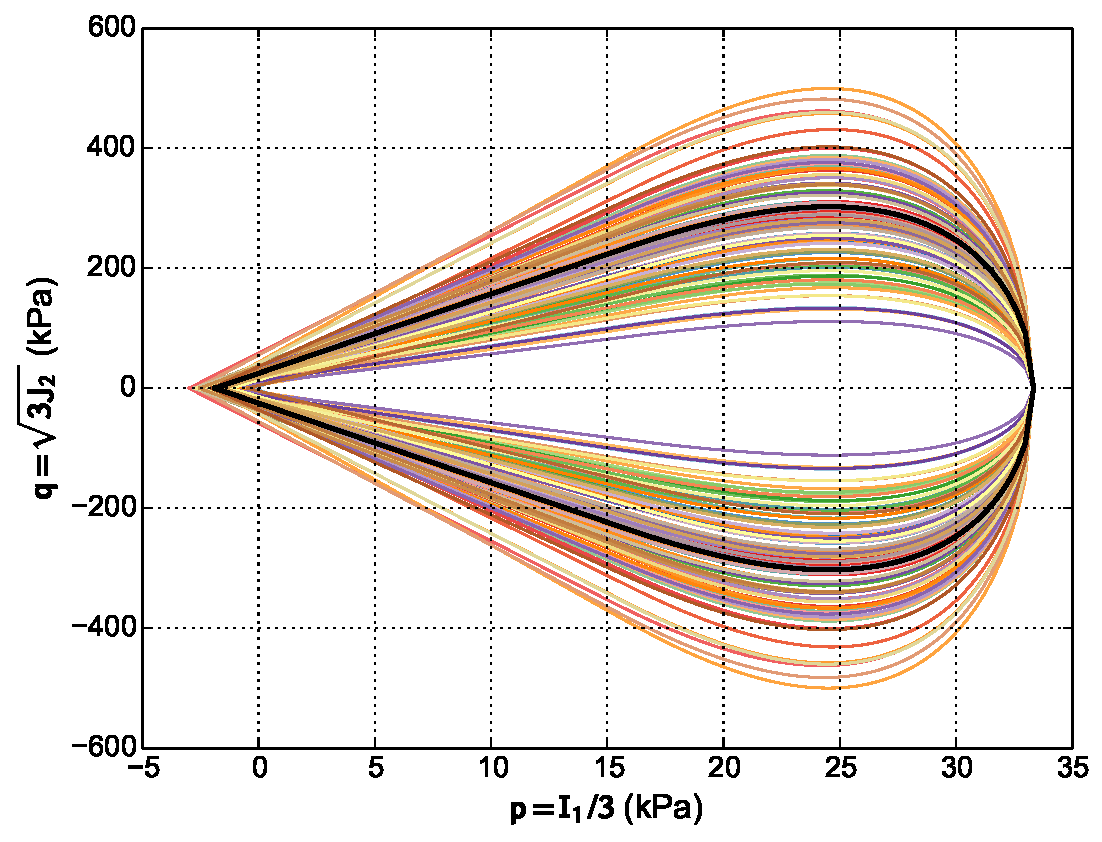
\includegraphics[width=0.9\textwidth]{FIGS/YieldSurfaceVariations.pdf}
  \caption{Variability in the yield surface by applying volume scaling and Weibull variability in 
           the yield surface parameters.  The median yield surface is shown by the black line.  The 
           median parameter values are \texttt{PEAKI1} = 1 kPa, \texttt{FSLOPE} = 0.453, \texttt{YSLOPE} = 0.31,
           \text{STREN} = 10 MPa.  The element volume is $10^{-6}$ m$^3$ while the reference volume is 
           $10^{-3}$ m$^3$. The Weibull modulus for all the parameters is 4.}
  \label{fig:yield_surf_var}
\end{figure}

\section{Density-dependence model} \label{app:density}
We use the Pabst-Gregorova model~\citep{Pabst2015} to scale the bulk and shear moduli.  For
the hydrostatic strength we use an ad-hoc model that is calibrated based on the high density
dry Mason sand SHPB tests.

Let $\phi_0$ be the initial porosity of the test material and let $\phi_\Tref$ be the initial porosity
of the reference material that was used to calibrate the bulk modulus parameters and the crush curve.
Following Pabst and Gregorova, we define a modulus scaling factor $K_{\text{fac}}$
\Beq
   K_{\text{fac}} = \exp\left[-\frac{\phi_0}{1 - \phi_0} + \frac{\phi_\Tref}{1 - \phi_\Tref}\right]
\Eeq
such that the bulk and shear moduli of the test material is
\Beq
   K_d \leftarrow K_{\text{fac}} K_d ~,\quad \Tand \quad
   G \leftarrow K_{\text{fac}} G  \,.
\Eeq
These scaled moduli are used in the partially saturated model.

For the hydrostatic strength we use the ad-hoc density scaling model
\Beq
  p_1 \leftarrow p_1\exp\left[\rho_{\text{fac}} K_{\text{fac}} (K_{\text{fac}} - 1)\right] 
\Eeq
where $p_1$ is the parameter of the crush curve model, and $\rho_{\text{fac}}$ is calibrated using 
high density data and has a value between 1 and 10.

Plots of the predicted and experimental SHPB test results for a range of initial Mason sand
densities are shown in the figures below.
\begin{figure}[htbp!]
  \centering
  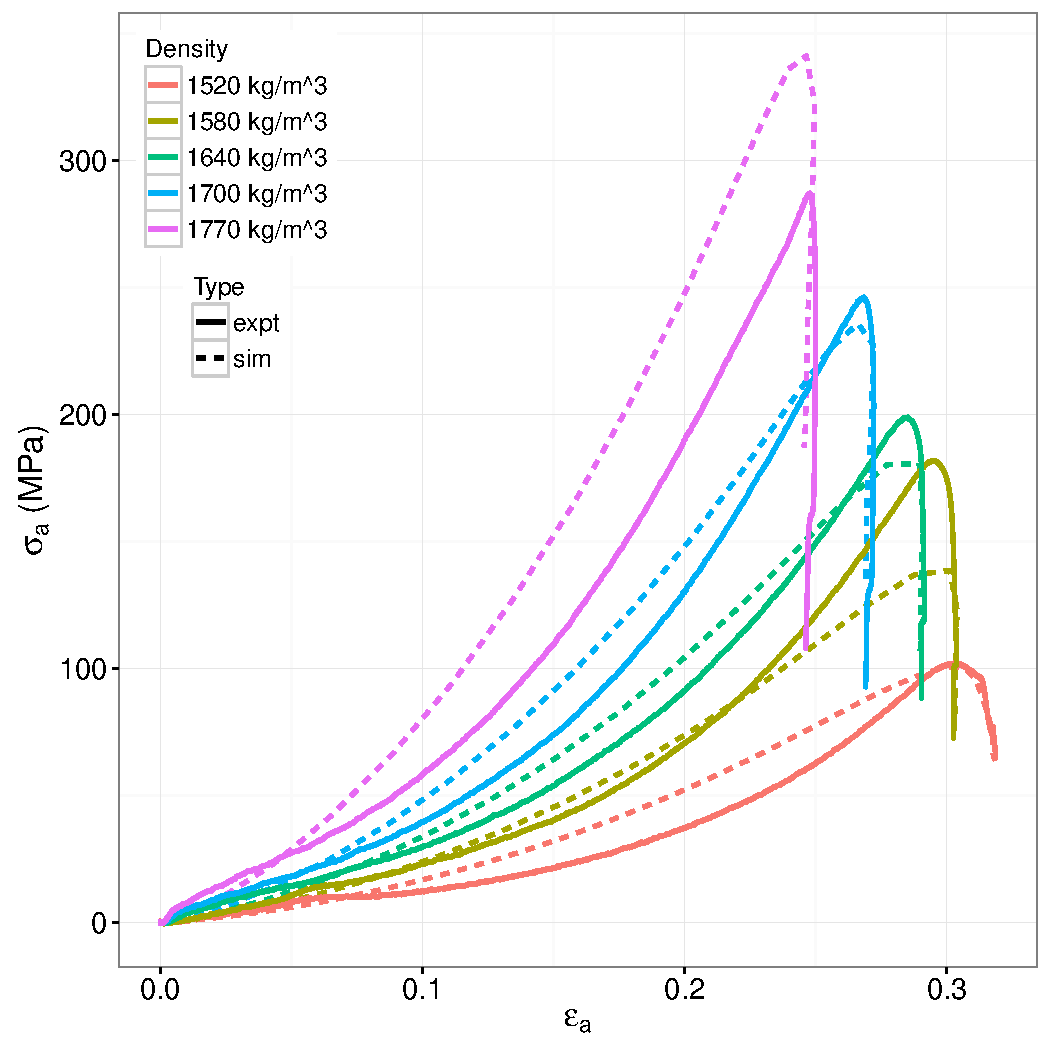
\includegraphics[width=0.5\textwidth]{FIGS/MasonSandSHPB_SaEa_sim_expt.pdf}
  \caption{Axial stress vs. axial strain in split-Hopkinson pressure bar: dry Mason sand: 
           Various initial densities.  We have used $\phi_\Tref = 0.42$ and $\rho_{\text{fac}} = 5$.}
  \label{fig:shpb_dry_Sa_density}
\end{figure}

\begin{figure}[htbp!]
  \begin{minipage}{0.5\textwidth}
    \centering
    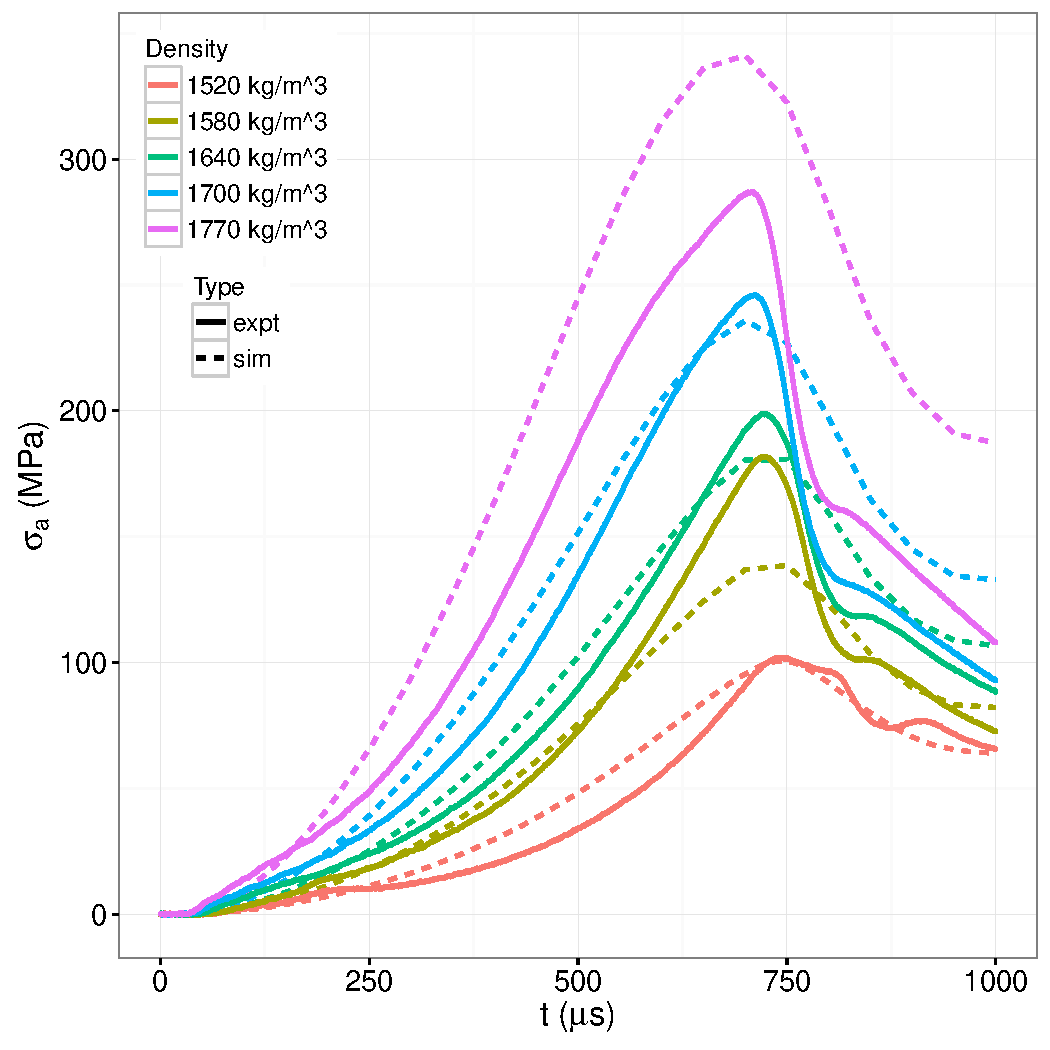
\includegraphics[width=0.9\textwidth]{FIGS/MasonSandSHPB_Sat_sim_expt.pdf}\\
    (a) Axial stress vs. time.
  \end{minipage}
  \begin{minipage}{0.5\textwidth}
    \centering
    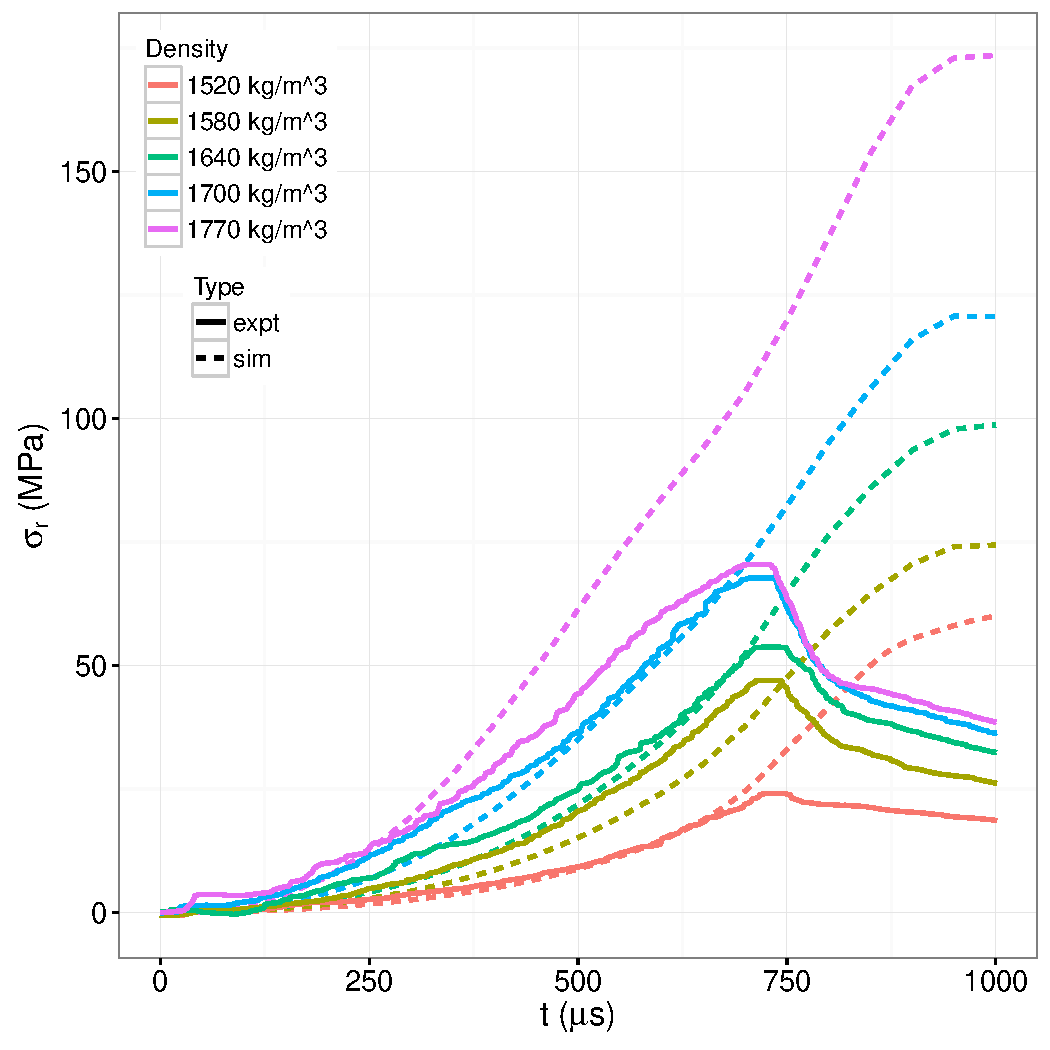
\includegraphics[width=0.9\textwidth]{FIGS/MasonSandSHPB_Srt_sim_expt.pdf}\\
    (b) Radial stress vs. time.
  \end{minipage}
  \caption{Axial stress and radial stress in split-Hopkinson pressure bar: dry Mason sand: 
           Various initial densities}
  \label{fig:shpb_dry_SaSr_density}
\end{figure}

\begin{figure}[htbp!]
  \begin{minipage}{0.5\textwidth}
    \centering
    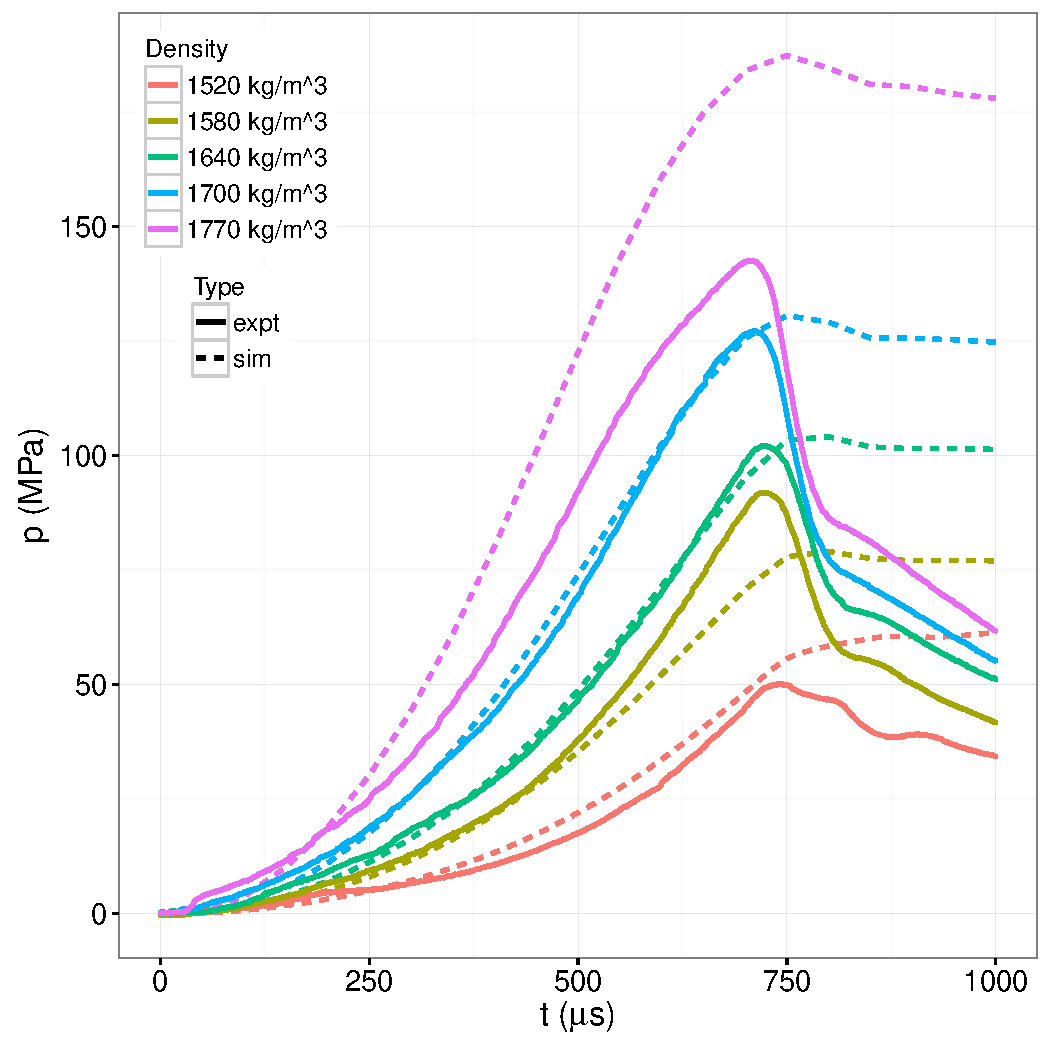
\includegraphics[width=0.9\textwidth]{FIGS/MasonSandSHPB_pt_sim_expt.pdf}\\
    (a) $p$ vs. time.
  \end{minipage}
  \begin{minipage}{0.5\textwidth}
    \centering
    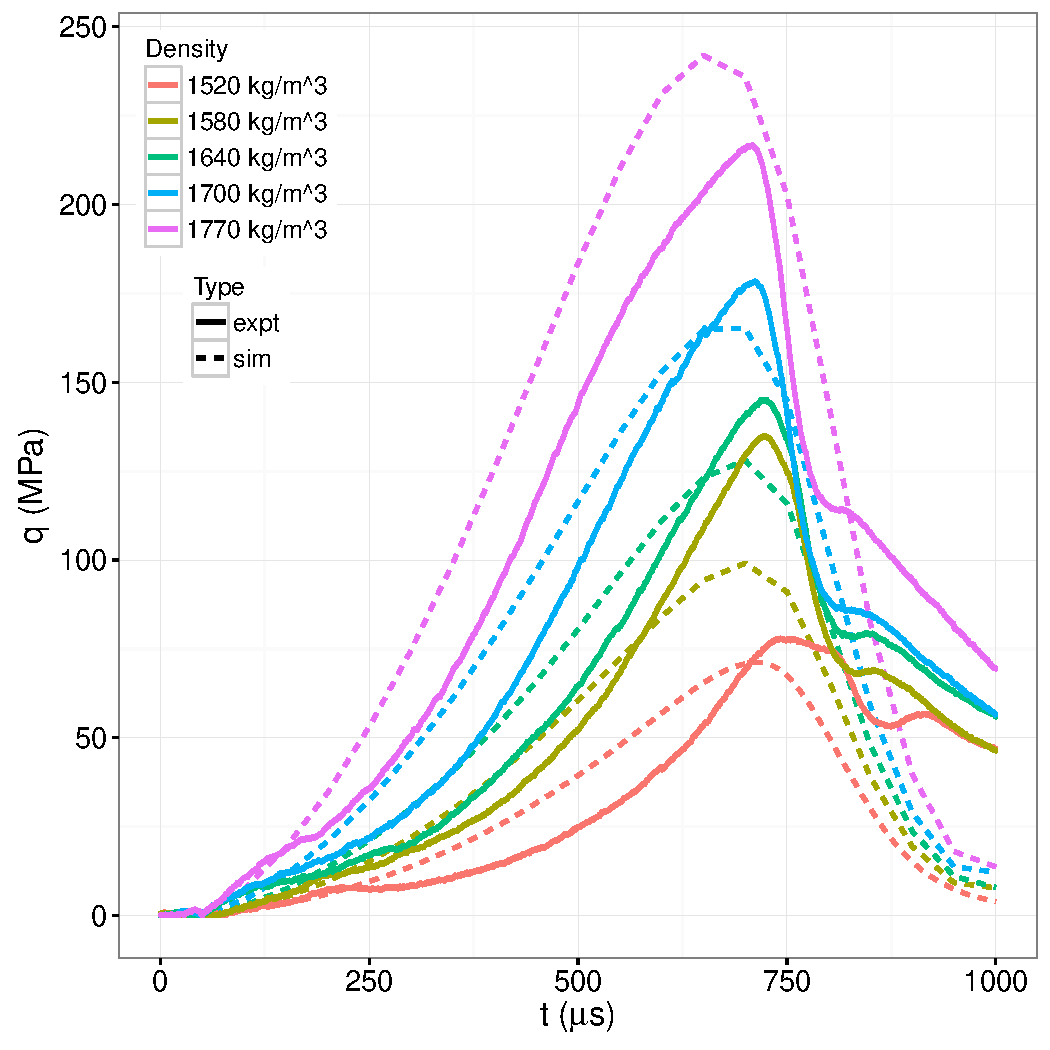
\includegraphics[width=0.9\textwidth]{FIGS/MasonSandSHPB_qt_sim_expt.pdf}\\
    (b) $q$ vs. time.
  \end{minipage}
  \caption{Axial stress and radial stress in split-Hopkinson pressure bar: dry Mason sand: 
           Various initial densities}
  \label{fig:shpb_dry_pq_density}
\end{figure}

\begin{figure}[htbp!]
  \begin{minipage}{0.5\textwidth}
    \centering
    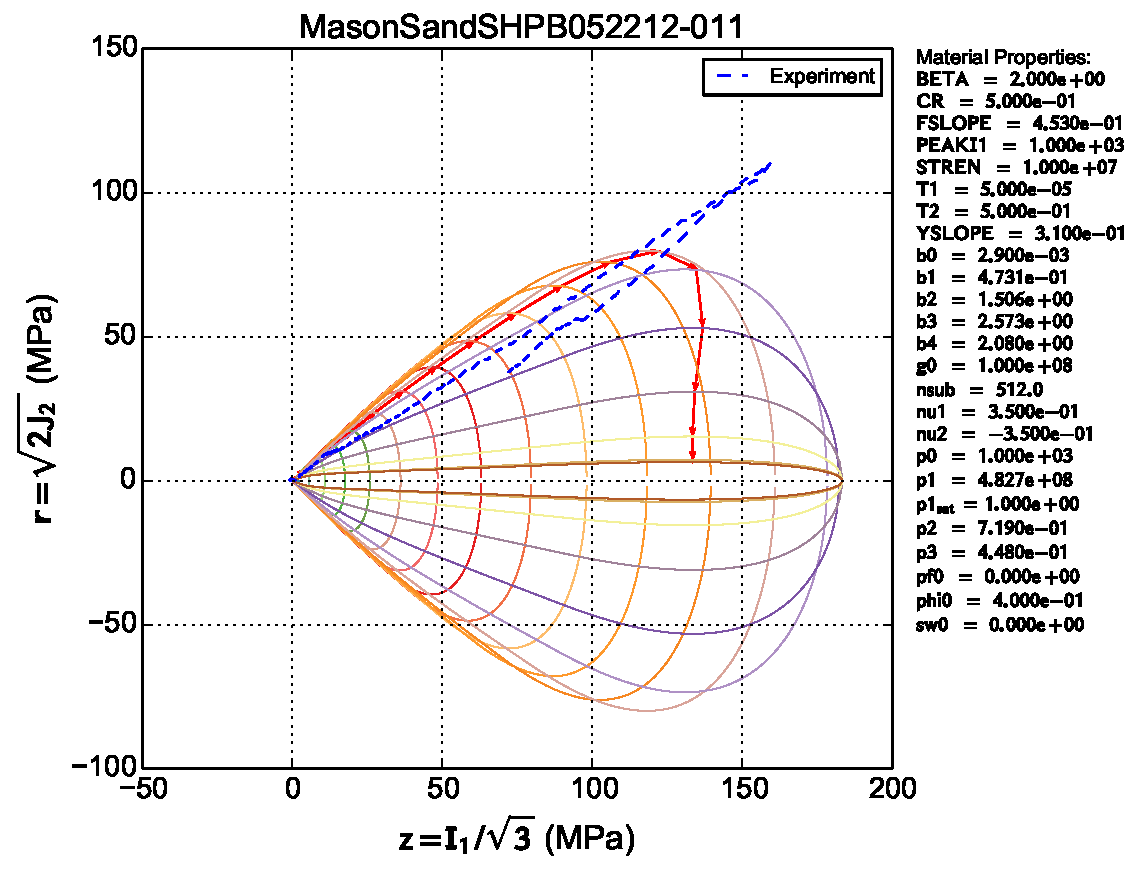
\includegraphics[width=0.9\textwidth]{FIGS/MasonSandSHPB052212-011_vs_expt_zr.pdf}\\
    (a) 1580 kg/m$^3$
  \end{minipage}
  \begin{minipage}{0.5\textwidth}
    \centering
    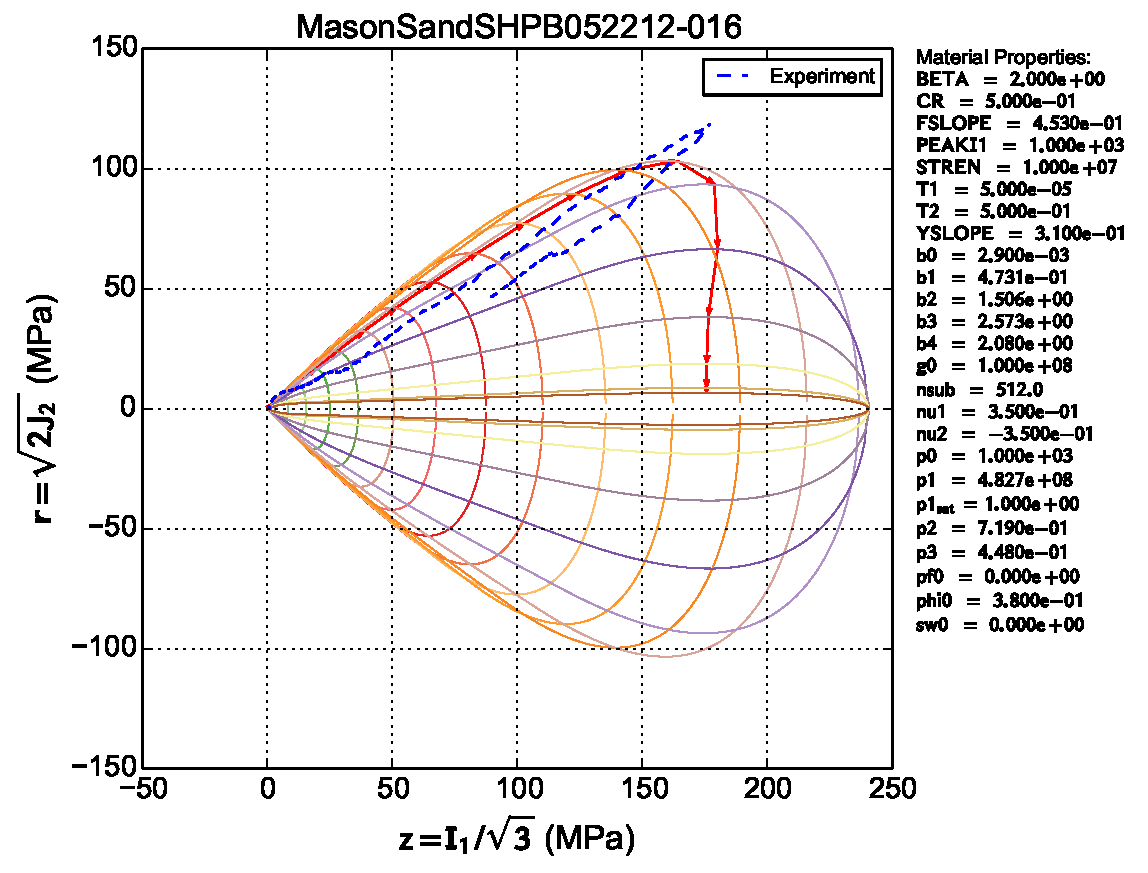
\includegraphics[width=0.9\textwidth]{FIGS/MasonSandSHPB052212-016_vs_expt_zr.pdf}\\
    (b) 1640 kg/m$^3$
  \end{minipage}
  \caption{Plot of stress path and yield surface in $z$-$r$ space.
           Moderate initial densities}
  \label{fig:shpb_dry_zr_density_0}
\end{figure}

\begin{figure}[htbp!]
  \begin{minipage}{0.5\textwidth}
    \centering
    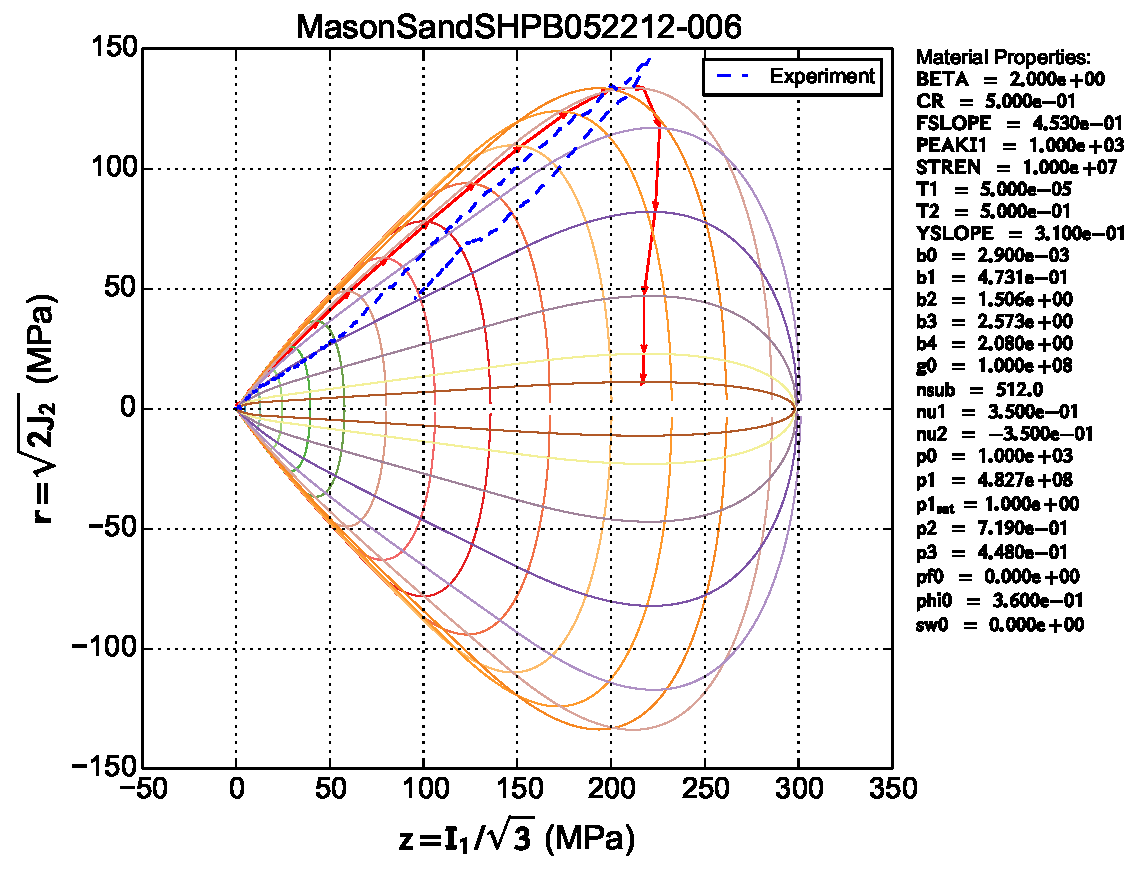
\includegraphics[width=0.9\textwidth]{FIGS/MasonSandSHPB052212-006_vs_expt_zr.pdf}\\
    (a) 1700 kg/m$^3$
  \end{minipage}
  \begin{minipage}{0.5\textwidth}
    \centering
    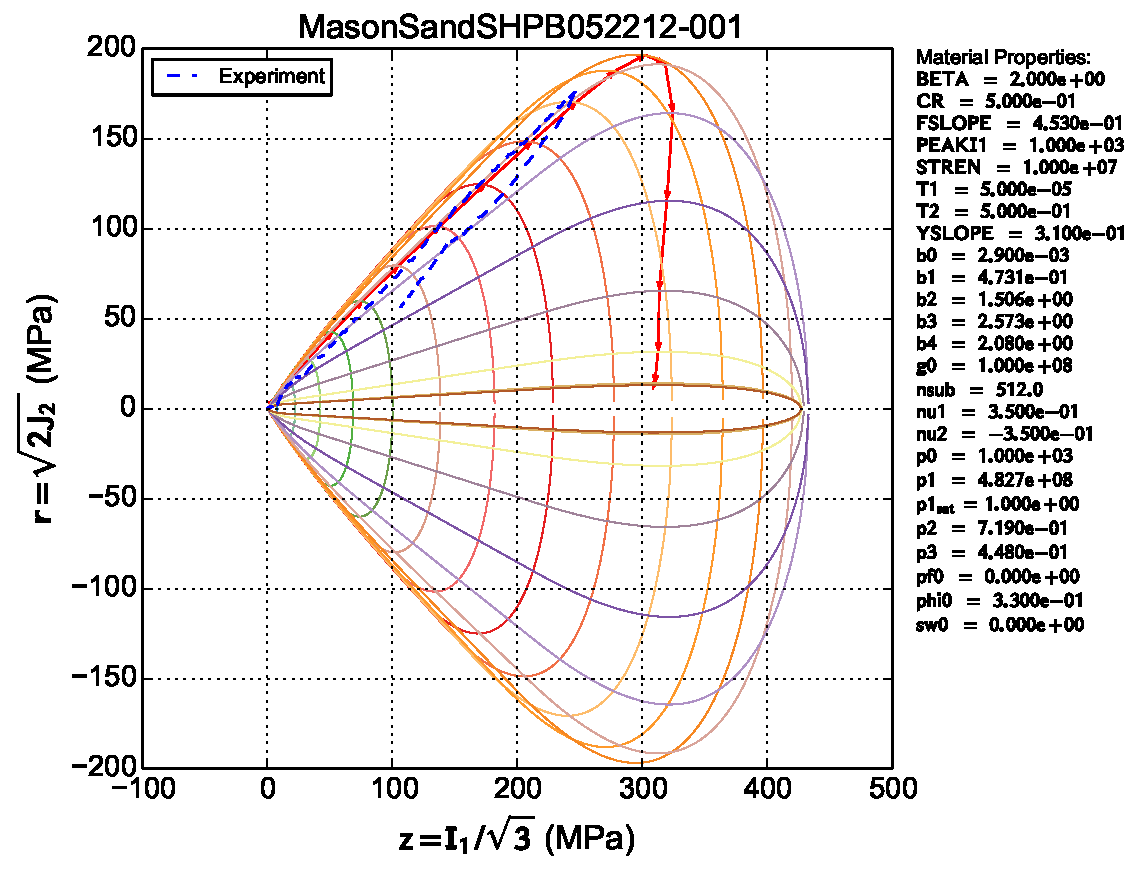
\includegraphics[width=0.9\textwidth]{FIGS/MasonSandSHPB052212-001_vs_expt_zr.pdf}\\
    (b) 1770 kg/m$^3$
  \end{minipage}
  \caption{Plot of stress path and yield surface in $z$-$r$ space.
           High initial densities}
  \label{fig:shpb_dry_zr_density_1}
\end{figure}


\section{Verifying stress paths for uniaxial strain loading} \label{app:qp}
Most of the simulations discussed in this report have been driven by uniaxial strain.
We can check that the code is doing the right thing by comparing the slope of the loading
path in $p$-$q$ space for elastic states.  This appendix discusses what we should expect
for linearly elastic materials.

From linear elasticity,
\Beq
  \Bsig = \lambda \Tr(\Bveps) \BI + 2 \mu \Bveps
\Eeq
where 
\Beq
   \lambda := K - \tfrac{2}{3} G \quad \Tand \quad \mu := G \implies K = \lambda + \tfrac{2}{3} \mu
\Eeq
and $K, G$ are the bulk and shear modulus, respectively. Therefore,
\Beq
  \Bal
  p & := \tfrac{1}{3} \Tr(\Bsig) = \left(\lambda + \tfrac{2}{3} \mu\right)\Tr(\Bveps) \\
  \BsT & := \Bsig - p \BI = \lambda \Tr(\Bveps) \BI + 2 \mu \Bveps - \left(\lambda + \tfrac{2}{3} \mu\right)\Tr(\Bveps) \BI = 2\mu \left[ \Bveps - \tfrac{1}{3} \Tr(\Bveps) \BI\right] \,.
  \Eal
\Eeq
From the second equation above, we can compute 
\Beq
  q := \sqrt{3J_2} = \sqrt{\tfrac{3}{2} \BsT:\BsT}
    = \sqrt{\tfrac{3}{2} (2\mu)^2 \left[ \Bveps:\Bveps - \tfrac{1}{3} [\Tr(\Bveps)]^2 \right]} 
    = 2\mu \sqrt{\tfrac{3}{2} \left[ \Bveps:\Bveps - \tfrac{1}{3} [\Tr(\Bveps)]^2 \right]} \,.
\Eeq
For uniaxial strain in the $1$-direction, $\Tr(\Bveps) = \Veps_{11}$ and $\Bveps:\Bveps = \Veps_{11}^2$, 
and the above equations for $p$ and $q$ become
\Beq
  p = \left(\lambda + \tfrac{2}{3} \mu\right)\Veps_{11} = K \Veps_{11} \quad \Tand \quad
  q = 2G \Veps_{11} \,.
\Eeq
Therefore, for uniaxial strain linear elastic deformations starting from zero strain, the slope of the 
loading path is
\Beq
  \frac{q}{p} = \frac{2G}{K} 
    = \frac{2}{K}\,\frac{3K(1 - 2\nu)}{2(1+\nu)} 
    = \frac{3(1 - 2\nu)}{1+\nu} \,.
\Eeq
For $\nu = 0.35$, the slope of the loading path is $\frac{2}{3}$ which can be used as a check of the 
algorithm.


\end{appendices}

\end{document}
